%% Computational Linguistics (COLI) journal template
%% MIT Press / Association for Computational Linguistics
%% Class file: clv2025.cls  |  Bib style: compling.bst
\documentclass[final]{clv2025}

\jvol{vv}
\jnum{nn}
\jyear{2026}

%% Document type — options: Long Paper, Short Paper, Survey,
%% Survey Proposal, Position Paper, Squibs and Discussions, Featured Article
\dochead{Long Paper}

%% To be filled upon acceptance (provided by editorial office)
\pageonefooter{Submission received: \textit{[date]}.}

\runningtitle{Evaluating LLM Adaptation to Sociodemographic Factors}
\runningauthor{Zhong, Li, Fan, and Sun}

%% Additional packages (T1 fontenc, amssymb, natbib, hyperref already in cls)
\usepackage[utf8]{inputenc}
\usepackage{amsmath}

%% Graphics and figures
\usepackage{graphicx}
\usepackage{float}
\usepackage{subfig}
\captionsetup[subfloat]{labelformat=empty}

%% Tables
\usepackage{booktabs}
\usepackage{array, multirow}
\usepackage{tabularx}

%% Other packages
\usepackage{xcolor}
\usepackage{enumitem}
\usepackage{xspace}
\usepackage{microtype}

%% Cross-referencing (must load after hyperref, which is in cls)
\usepackage[capitalize]{cleveref}
\crefname{section}{Sec.}{Secs.}
\Crefname{section}{Section}{Sections}
\Crefname{table}{Table}{Tables}
\crefname{table}{Tab.}{Tabs.}

%% Custom commands
\newcommand{\paratitle}[1]{\smallskip\noindent\textbf{#1}}
\newcommand{\eg}{\textit{e.g.,}\xspace}
\newcommand{\Eg}{\textit{E.g.,}\xspace}
\newcommand{\ie}{\textit{i.e.,}\xspace}
\newcommand{\etal}{\textit{et al.}\xspace}

%% Colored box for prompt examples
\usepackage{tcolorbox}
\definecolor{lightroyalblue}{HTML}{EBEBEC}
\definecolor{cc1}{RGB}{155, 65, 70}
\newtcolorbox{abox}{colback=lightroyalblue, colframe=lightroyalblue}

\begin{document}

\title{Evaluating LLM Adaptation to Sociodemographic Factors:\\
User Profile vs.\ Dialogue History}

\author{Qishuai Zhong\thanks{Corresponding author.}$^{,1}$,
        Zongmin Li$^{1}$,
        Siqi Fan$^{2}$,
        Aixin Sun$^{1}$}

\affilblock{
    \affil{College of Computing and Data Science, Nanyang Technological University, Singapore\\
           \quad \email{qishuai.zhong@ntu.edu.sg}}
    \affil{University of Electronic Science and Technology of China, Chengdu, China}
}

\maketitle

\begin{abstract}
Effective engagement by large language models (LLMs) requires adapting responses to users' sociodemographic characteristics, yet most evaluations focus on single-turn prompts with user attributes, despite real-world systems relying on richer interaction formats such as dialogue history. We propose a unified framework to evaluate LLM adaptation across interaction formats in which demographic information is presented either within a single turn or accumulated through multi-turn dialogue context. Beyond alignment accuracy, we introduce individual preservation metrics to assess whether models preserve user-specific variation. To support this evaluation, we employ a multi-agent pipeline to generate synthetic dialogues paired with user profiles and probe value expression using World Values Survey questions \citep{Haerpfer2020-qe}. Experiments on LLMs reveal three findings: (1) high alignment accuracy is often achieved through demographic homogenization rather than genuine personalization; (2) increased model scale improves average alignment accuracy while degrading individual preservation; and (3) response consistency across interaction formats does not imply preservation consistency. These results show that effective value alignment requires preserving individual diversity, not merely matching group-level patterns.
\end{abstract}

\setcounter{secnumdepth}{4}

%====================
\section{Introduction}
\label{sec:introduction}

Large Language Models (LLMs) and their chatbot applications have attracted widespread attention since the release of ChatGPT \citep{openai2024gpt4technicalreport, dam2024completesurveyllmbasedai}. Advances in open-source frameworks \citep{wolf2020huggingfaces, vllm} have further enabled on-premises deployment across diverse domains. In real-world applications, effective engagement increasingly requires LLMs to tailor responses to users' sociodemographic characteristics and associated cultural or ethical preferences \citep{sicilia2024humbelhumanintheloopapproachevaluating, altenburger2024examiningrolerelationshipalignment}.

\begin{figure}[H]
\begin{center}
    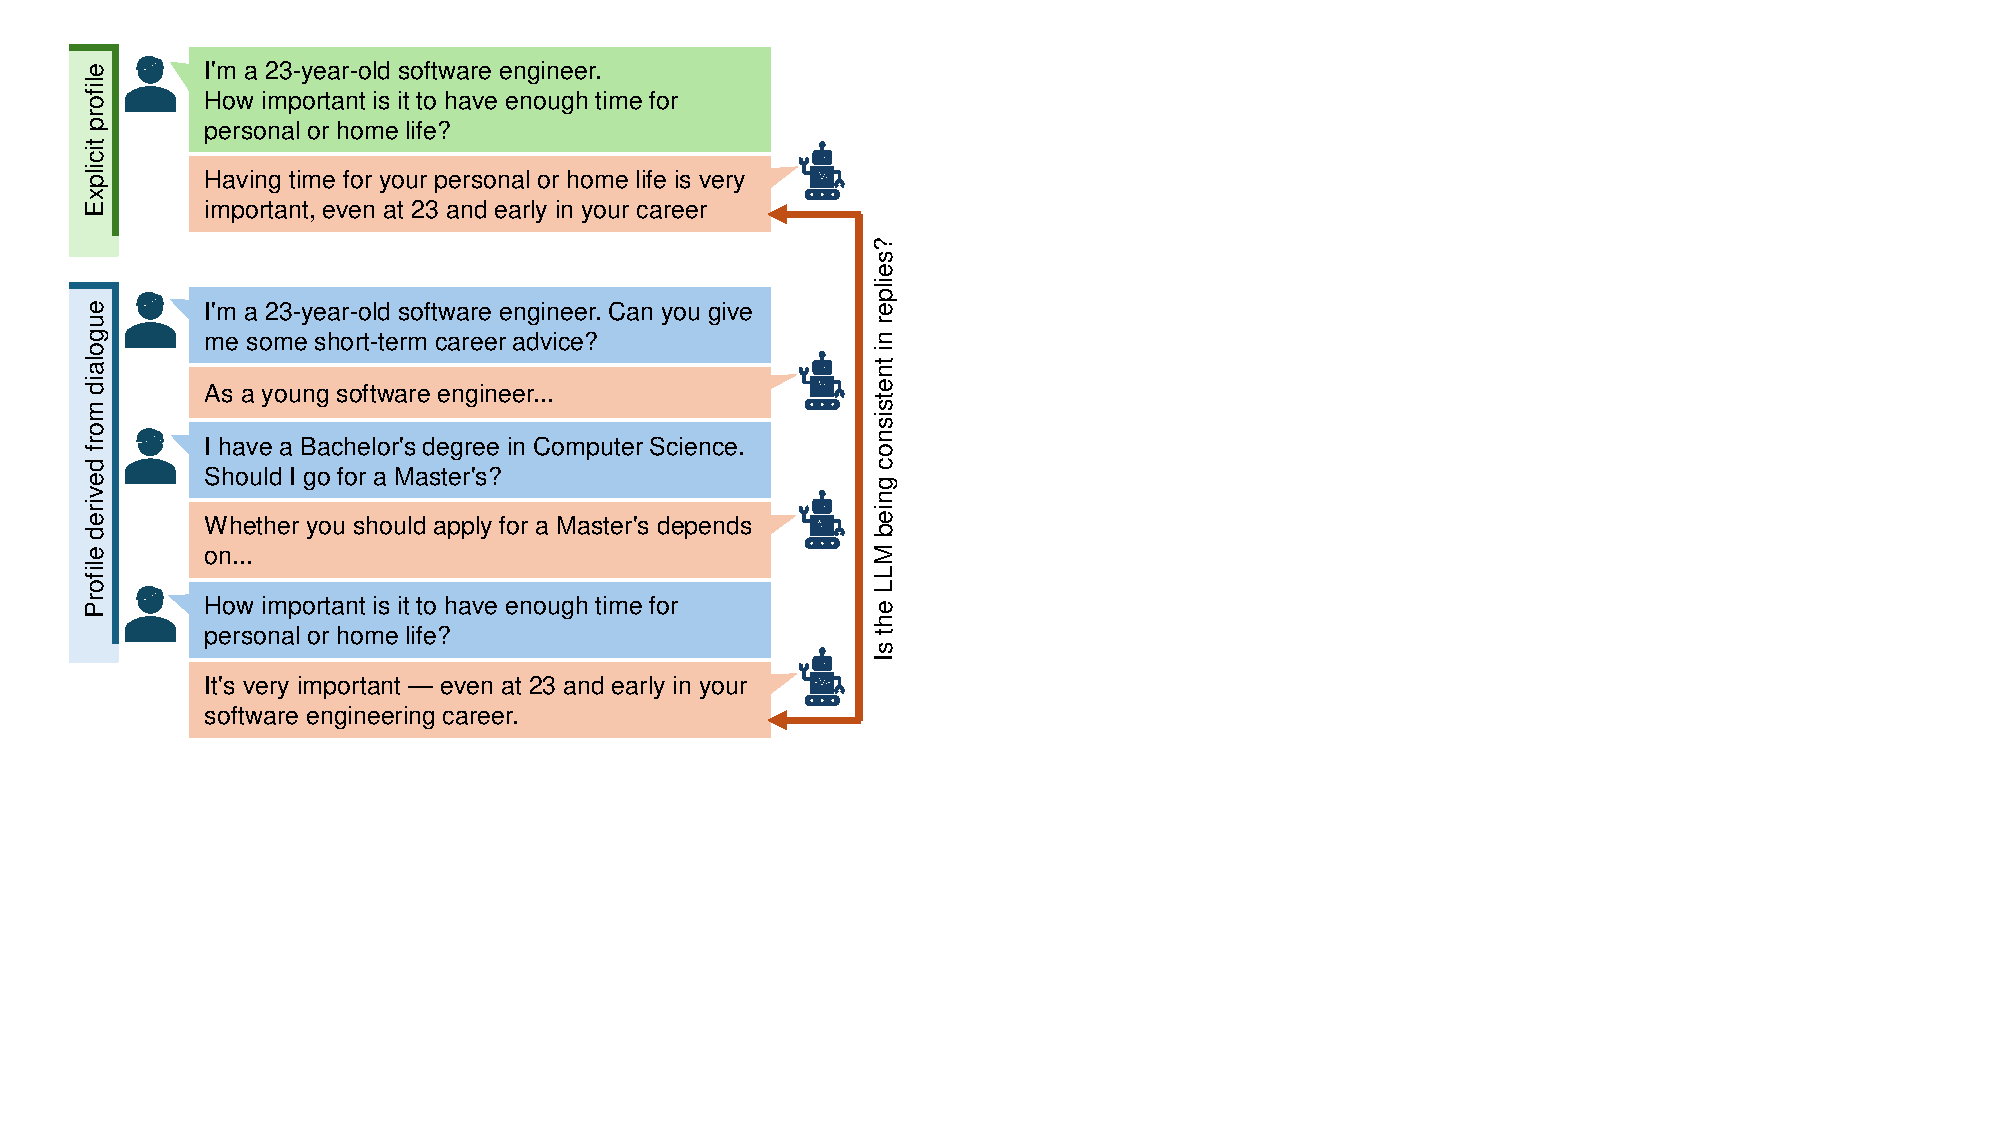
\includegraphics[width=0.45\textwidth]{figures/PersonaExample.pdf}
    \caption{Overview of our evaluation framework. Given identical user demographics presented via explicit profiles (top) or embedded in dialogue history (bottom), we assess: (1) whether models adapt their value expressions to user attributes, (2) whether adaptations align with human patterns, (3) whether alignment is achieved through genuine personalization or demographic homogenization, and (4) whether these properties remain consistent across formats.}
\label{fig:research_target}
\end{center}
\end{figure}

Unlike humans, who generally maintain stable values and social norms across contexts \citep{HumanStableValues, relativeconsistenthumanvalues}, LLMs exhibit variability in their expressed values due to human-generated training data and contextual cues \citep{kharchenko2024llmsrepresentvaluescultures, kovač2024large}. While such flexibility enables personalization, prior work in psychology, sociolinguistics, and AI shows that adapting behavior based on demographic generalizations can reinforce harmful stereotypes by collapsing individual users into homogeneous group representations \citep{bennett2014stereotypes, cheng2023markedpersonas, lee2023culturalbias}. To balance personalization with alignment, LLMs should adapt their responses to reflect individual users while remaining consistent with socially grounded value patterns, rather than collapsing individuals into demographic prototypes. We refer to this capability as \textbf{behavioral adaptation}, defined as a model's ability to adjust its expressed value positions in response to user sociodemographic signals without sacrificing individual-level diversity.

Sociodemographic attributes such as age, education, occupation, and socioeconomic status are strongly correlated with cultural norms and value orientations \citep{Fung2016-re, genderandvalues, Gelfand2011-ei}. Recent studies have examined value alignment between LLMs and user profiles \citep{yao2024claveadaptiveframeworkevaluating, zhang2024heterogeneousvaluealignmentevaluation, sukiennik2025evaluationculturalvaluealignment}. However, most evaluations focus on single-turn settings where demographic attributes are explicitly provided (Figure~\ref{fig:research_target}, top), leaving open whether LLMs maintain consistent adaptation when the same characteristics must be inferred from dialogue history (Figure~\ref{fig:research_target}, bottom).

In this work, we propose a unified framework to evaluate LLM behavioral adaptation across both interaction formats. Our evaluation addresses a progression of increasingly nuanced questions:
\begin{enumerate}
    \item \textbf{Adaptation}: Do LLMs adjust their expressed values in response to user sociodemographic characteristics?
    \item \textbf{Alignment}: Do such adaptations align with human response patterns?
    \item \textbf{Preservation}: Is alignment achieved through genuine personalization, or by collapsing individuals toward demographic homogenization?
    \item \textbf{Consistency}: Do adaptation and preservation remain stable across interaction formats?
\end{enumerate}

Questions (1) and (2) establish baseline adaptation capability; question (3) introduces \textit{individual preservation} analysis that reveals \textit{how} alignment is achieved; question (4) synthesizes these dimensions to assess cross-format behavioral stability. Since existing benchmarks lack dialogue datasets with aligned demographic annotations, we develop an agent-based pipeline to generate controlled user-chatbot dialogues \citep{dam2024completesurveyllmbasedai}. Our contributions are:

\begin{itemize}
    \item We propose a unified evaluation framework spanning multiple text interaction formats, with \textbf{individual preservation metrics} that distinguish genuine personalization from demographic homogenization.
    \item We design an agent-based workflow to generate sociodemographically aligned dialogues for controlled cross-format evaluation.
    \item We benchmark six open-source LLMs using the World Values Survey \citep{Haerpfer2020-qe}, revealing how adaptation, alignment, and preservation interact across formats.
\end{itemize}

Our experiments yield three central findings that build upon each other. First, models do adapt their values based on demographics, and these adaptations generally align with human patterns. However, we find that high alignment accuracy is frequently achieved through \textit{homogenization}, where models collapse individuals toward demographic group centroids rather than preserving individual diversity. Second, we observe a \textit{scaling paradox}: larger models achieve higher alignment accuracy but exhibit worse individual preservation. Third, synthesizing across formats, we find that response-level consistency does not imply preservation consistency---models producing similar outputs across formats can exhibit markedly different homogenization behaviors. Together, these findings demonstrate that effective value alignment requires preserving individual diversity, not merely optimizing aggregate accuracy.

%====================
\section{Literature Review}
%====================

This study examines LLM behavior adaptation in multi-turn human-model interactions and assesses value consistency across profile presented conditions. Given its intersection with persona attribute extraction and cultural value alignment in LLMs, we survey related work in both fields.

\subsection{Persona Attributes Understanding}

Evaluations of language models' understanding of persona attributes typically center on two tasks: next-utterance prediction and persona expansion. Standard benchmarks such as PersonaChat \citep{personachat}, RealPersonaChat \citep{realpersonachat}, and FaithfulPersonaChat \citep{faithfulPersonaChat} provide dialogues annotated with descriptive persona statements (\eg ``I'm a pet lover'') for these tasks. Other efforts, like Pchatbot \citep{pchatbot}, compile large-scale Chinese dialogues from Weibo and judicial forums but lack explicit demographic mappings. LiveChat \citep{gao-etal-2023-livechat} augments live-stream conversations with streamer personas that include demographic attributes, yet this information serves only as auxiliary context for next-utterance prediction.

Despite these resources, most existing datasets embed persona descriptions rather than well-defined sociodemographic profiles, limiting controlled analysis of LLM adaptation to quantifiable attributes. While grouping by attributes such as age is straightforward, contrasting more abstract traits (e.g., ``running enthusiast'' versus ``someone who lost a dog'') leads to unreliable or non-comparable groupings. More fundamentally, these datasets lack the controllability required for counterfactual comparisons across identical demographic attributes presented in different interaction formats. To address these limitations, we construct a synthetic dataset specifically designed to support rigorous evaluation of sociodemographic adaptation.



%=====================================
\subsection{Evaluating Values of Models}
%=====================================

A growing body of work evaluates how LLMs express social and cultural values under different prompting conditions. A common approach employs established survey instruments such as Hofstede's Value Survey Module (VSM) \citep{vsm2013-jj}, which has been used to probe cultural alignment in prior studies \citep{kharchenko2024llmsrepresentvaluescultures, arora2023probing, masoud-etal-2025-cultural}. Despite methodological differences, these works consistently show that LLMs adjust value expressions in response to contextual cues.

Other studies construct evaluation benchmarks based on the World Values Survey (WVS) \citep{Haerpfer2020-qe}. GlobalOpinionQA \citep{durmus2024towards} combines WVS and Pew survey questions, finding that many LLMs disproportionately reflect Western perspectives. WorldValueBench \citep{zhao2024worldvaluesbenchlargescalebenchmarkdataset} focuses on demographic conditioning and reveals that even advanced models struggle to capture the nuances of multicultural value systems. Together, these results suggest that while LLMs can modulate value expressions, alignment often remains coarse and group-level.

Recent work has further examined value expression under specific settings. BiasLens \citep{li2024benchmarkingbiaslargelanguage} evaluates social biases through role-playing scenarios, while \cite{moore-etal-2024-large} studies value consistency across prompt variations, observing generally stable model outputs. \cite{liu2025llmsgraspimplicitcultural} introduces a benchmark for assessing whether LLMs can infer implicit cultural values from natural conversational contexts, highlighting challenges in nuanced attitude detection and open-ended cultural reasoning.


Unlike prior studies, we analyze LLMs' value expression patterns using multi-turn human--model interactions, which better reflect real-world chatbot inputs. We also evaluate behavioral consistency when sociodemographic attributes are provided in the single-turn prompt versus within the dialogue.


Beyond value alignment, related work on \textbf{linguistic accommodation} examines how LLMs adapt their conversational style during interaction. Studies such as \cite{Chang_Wang_2025} show that models and users gradually converge in tone, while \cite{blevins2025languagemodelsaccommodateusers} find that models often over-accommodate stylistically, exceeding human baselines. Although stylistic accommodation differs from value adaptation, these findings highlight a parallel risk of over-adaptation in multi-turn settings, reinforcing group-level patterns rather than individual variation.

%==============================
\section{Research Targets}
\label{sec:research_targets}
%==============================

We define \emph{behavior adaptation capability} as a model's ability to adjust its \textbf{expressed value} in accordance with users' sociodemographic attributes. A central goal of this study is to examine whether such adaptation remains consistent when the same demographic information is provided in a single-turn prompt versus inferred from prior dialogue context (see Figure~\ref{fig:research_target}).


\subsection{Hypothesis}

We hypothesize that large language models adjust their value-oriented responses in response to users' sociodemographic attributes, with larger demographic differences inducing stronger behavioral shifts. We further hypothesize that these shifts broadly align with known patterns of value variation in human populations and remain stable across text-based interaction formats. Finally, we hypothesize that apparent alignment may be achieved either through individual-specific personalization or through convergence toward demographic group averages, which we term \emph{homogenization}.


\subsection{Values Assessment Instrument}

Following prior work \citep{durmus2024towards, jiang2024can, zhao2024worldvaluesbenchlargescalebenchmarkdataset}, we adopt the World Values Survey (WVS) \citep{Haerpfer2020-qe}, a standardized instrument for measuring human values, to evaluate behavioral adaptation of language models. WVS comprises 256 multiple-choice questions across 12 thematic categories reflecting diverse aspects of human values, such as \textit{Social Values, Norms, and Stereotypes}, \textit{Economic Values} and \textit{Perceptions of Corruption}.


We randomly sample \textbf{1,000 anonymized interviewee profiles} from the test split of WorldValueBench \citep{zhao2024worldvaluesbenchlargescalebenchmarkdataset}, a benchmark derived from WVS, to construct the \textit{seed dataset} $U$. Each profile is annotated with key sociodemographic attributes. The corresponding human responses serve as empirical reference distributions for value expression. To focus on value-oriented reasoning, we exclude the \textit{Happiness and Wellbeing} category due to its emotional and health-related content. From the remaining categories, we randomly select five questions per category, yielding 55 multiple-choice items denoted as the question set $Q$.\footnote{\url{https://anonymous.4open.science/r/llm_behavior_adaption-4591/datasets/wvs_benchmarks/picked_questions.json}} Each question includes discrete answer options labeled by \texttt{option\_id}, allowing both humans and models to select the most appropriate response. The number of options per question ranges from 2 to 10.

\subsection{Evaluation Scenarios}


Our evaluation framework builds progressively through three dimensions, each revealing deeper aspects of model behavior.

\paratitle{Adaptation \& Alignment.}
We first assess whether models adapt their expressed values to user demographics and whether these adaptations align with human patterns. We evaluate this across two interaction formats:
\begin{itemize}
    \item \textbf{\texttt{BA\_user}}: Models receive explicit user profiles specifying sociodemographic attributes (e.g., ``age: 23, job title: data scientist, education: Bachelor's degree'').
    \item \textbf{\texttt{BA\_dialogue}}: Models infer user attributes from dialogue history \citep{gupta-etal-2024-llm}, reflecting real-world conversational settings.
\end{itemize}
For both formats, we quantify alignment using \textit{Value Alignment Accuracy} (VAA), defined as the Pearson correlation between model-generated and corresponding human reference value vectors. Higher VAA indicates stronger alignment with human value patterns.


\paratitle{Individual Preservation.}
While adaptation metrics measure \textit{whether} models align with humans, they do not reveal \textit{how} this alignment is achieved. A model could achieve high VAA either through genuine personalization or by collapsing all individuals toward demographic group averages. To distinguish these mechanisms, we introduce individual preservation metrics that detect homogenization, variance collapse, and bias amplification. This distinction is critical: group-level alignment alone cannot distinguish personalization from demographic stereotyping.

\paratitle{Cross-Format Consistency.}
Finally, we synthesize across interaction formats to assess behavioral stability. We evaluate consistency at both the response level (do models produce similar outputs across formats?) and the preservation level (do homogenization patterns remain stable?). A key question is whether surface-level response similarity implies consistency in preservation properties, or whether these dimensions can decouple.

\begin{figure}[H]
\begin{center}
    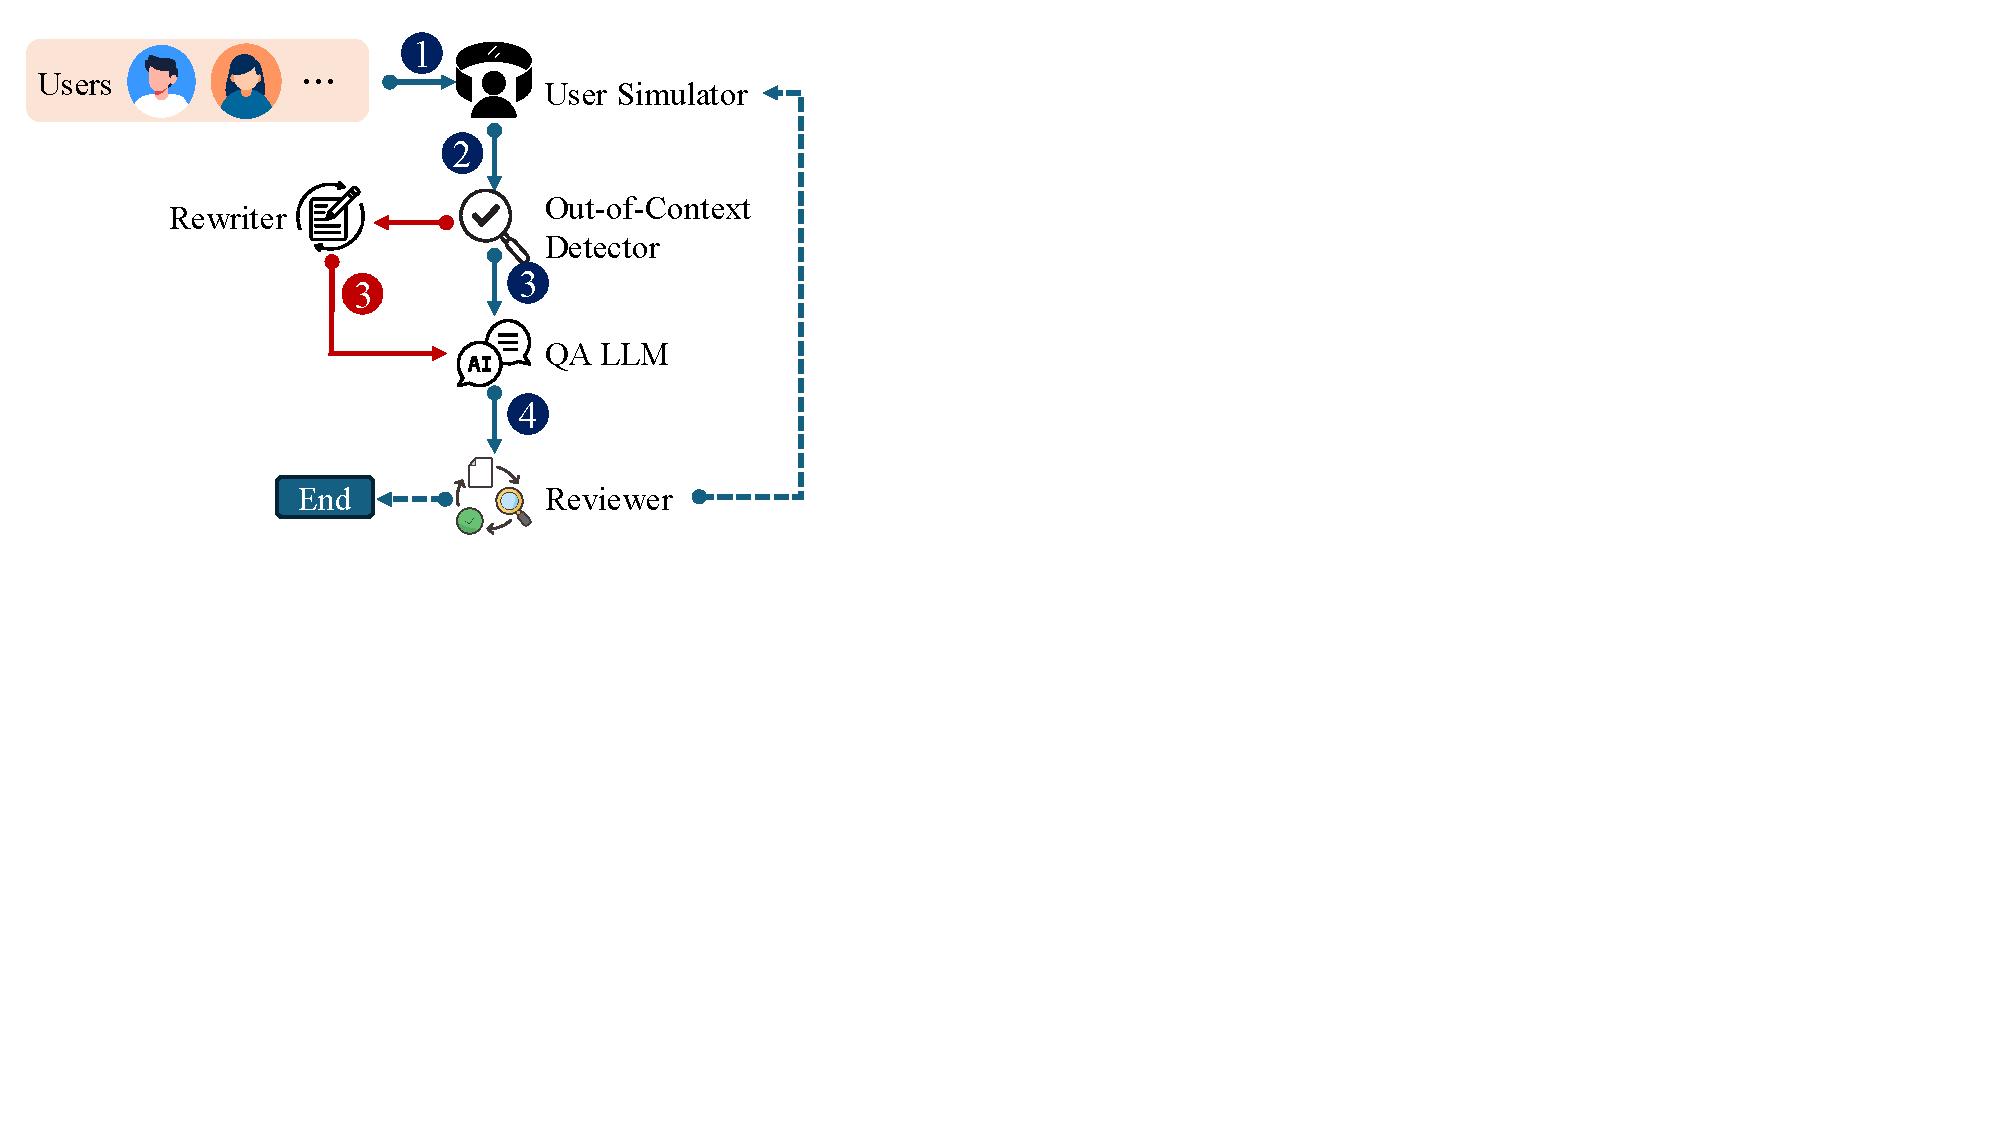
\includegraphics[trim=0.5cm 10cm 19.5cm 0.5cm,clip=true,width=0.45\textwidth]{figures/dialogue_dataset_geneartion/DataGen_new.pdf}
    \caption{Architecture of the agentic dataset generation framework. In each iteration: (i) the \textbf{User Simulator} LLM produces a user-style question conditioned on the user's profile; (ii) the \textbf{Out-of-Context Detector} assesses the question's consistency with the user's context; (iii) the \textbf{QA LLM} generates an answer for validated questions, while the \textbf{Rewriter} revises those detected as out-of-context; and (iv) the \textbf{Reviewer} evaluates the interaction to determine whether the dialogue objectives have been fulfilled and the session can be concluded.}
\label{fig:conversation_generation}
\end{center}
\end{figure}

%============================
\section{Dialogue Datasets Generation}
\label{sec:generating_dialogue}

While \texttt{BA\_user} assessment is straightforward, evaluating \texttt{BA\_dialogue} and \texttt{Consistency} is hindered by the absence of datasets meeting two key criteria: (1) human-model dialogues with organically embedded demographic attributes, and (2) explicit mappings between each dialogue and its corresponding user profile.

Inspired by prior work on synthetic dialogue generation \citep{abdullin2024syntheticdialoguedatasetgeneration, chen-etal-2024-diahalu}, we propose a multi-role agentic framework for constructing large-scale synthetic dialogue corpora grounded in demographic information. Our pipeline follows a controlled generation schema, where each user profile $u \in U$ serves as a generation seed. The sampled profiles represent a diverse range of sociodemographic backgrounds. Each dialogue instance is explicitly conditioned on a unique user profile, embedding quantifiable attributes (including age, highest education level, occupational group, region of residence, socioeconomic class, and immigrant status) within contextually coherent interactions.


To constrain the generative space while ensuring the natural incorporation of demographic cues, we restrict the conversational domains to two representative scenarios: \textbf{career guidance} and \textbf{investment advice}. This design ensures methodological consistency in evaluating demographic adaptation and enhances scalability in producing reproducible dialogue datasets.

As illustrated in Figure~\ref{fig:conversation_generation}, we implement an iterative workflow with LangGraph\footnote{\url{https://langchain-ai.github.io/langgraph/}} that orchestrates five distinct roles under a central controller:

\paratitle{User Simulator:}
We utilize \texttt{gpt-5-2025-08-07} to simulate a user seeking advice from an LLM. Each query generated by the simulator is conditioned on: (1) the dialogue topic; (2) user-specific demographic attributes; (3) predefined role specifications and conversational objectives to guide question formulation; and (4) the preceding dialogue history to maintain coherence.

\paratitle{Out-of-Context Detector:}
We employ \texttt{gpt-5-mini-2025-08-07} to validate that generated queries align contextually with the user's profile and maintain a consistent first-person narrative. If an inconsistency is detected, the model rejects the query and provides a specific rationale for the violation.

\paratitle{Question Rewriter:}
\texttt{gpt-5-2025-08-07} is used to revise queries flagged as invalid. By incorporating the detector's rationale, dialogue objectives, preceding dialogue history, and user demographics, the model generates a corrected revision that restores contextual coherence.

\paratitle{Question Answering (QA) LLM:}
\texttt{gpt-o4-mini-2025-04-16} \citep{openai2024gpt4technicalreport} serves as the respondent, using its default configuration to ensure naturalistic output. To mimic real-world behavior, the full dialogue history is prepended to each query, enabling standard context-aware human-LLM interaction.

\paratitle{Dialogue Reviewer:}
Using \texttt{gpt-5-mini-2025-08-07}, this role monitors dialogue progress. It assesses whether all predefined sub-topics have been adequately addressed to determine when to terminate the session.

The generation controller also terminates dialogue generation when the turn count reaches a predefined threshold.

For each topic, 1{,}000 dialogue sets are generated, denoted as $D_{c}$ for career guidance\footnote{\url{https://anonymous.4open.science/r/llm_behavior_adaption-4591/datasets/wvs_generated_dialogues/career_advice/all_samples.jsonl}}, and $D_{i}$ for investment advice\footnote{\url{https://anonymous.4open.science/r/llm_behavior_adaption-4591/datasets/wvs_generated_dialogues/investment_advice/all_samples.jsonl}}. Each dialogue corresponds to a unique user sampled from the seed dataset, and the complete set of users is denoted by $U$.




%======================================
\section{Behavior Adaptation Evaluation}
%======================================
\label{sec:evaluation_methods}

Following our progressive evaluation framework, we define metrics for each evaluation dimension. Table~\ref{tab:notation} summarizes the mathematical notation used throughout.

\subsection{Adaptation \& Alignment Metrics}

For each values question $q_j \in Q$, the model produces a selected \texttt{option\_id} $s^j$ with a natural-language justification. We require justifications rather than stand-alone option selection, which yields unreliable evaluations \citep{kabir2025breakcheckboxchallengingclosedstyle}. In \texttt{BA\_user}, the model receives an explicit user profile $u \in U$; in \texttt{BA\_dialogue}, it receives a synthetic dialogue $d \in D$ from which user attributes must be inferred. Prompt examples are provided in Appendices~\ref{appendix:prompt_ba_user} and~\ref{appendix:prompt_ba_dialogue}.

In \texttt{BA\_user}, responses for a given profile $u$ across all questions form the vector $S_u = [s^1_u, \dots, s^m_u]$, where $s^j_u$ is the selected option for question $q_j$. Aggregating over all profiles yields $\mathcal{S}_U \in \mathbb{R}^{|U| \times m}$. In \texttt{BA\_dialogue}, responses for a given dialogue $d$ form $S_d = [s^1_d, \dots, s^m_d]$, where each $s^j_d$ reflects the user attributes inferred from $d$. Aggregating over all dialogues yields $\mathcal{S}_D \in \mathbb{R}^{|D| \times m}$. The querying workflow is illustrated in Figure~\ref{fig:querying_model_workflow}.


\begin{figure}[H]
\begin{center}
    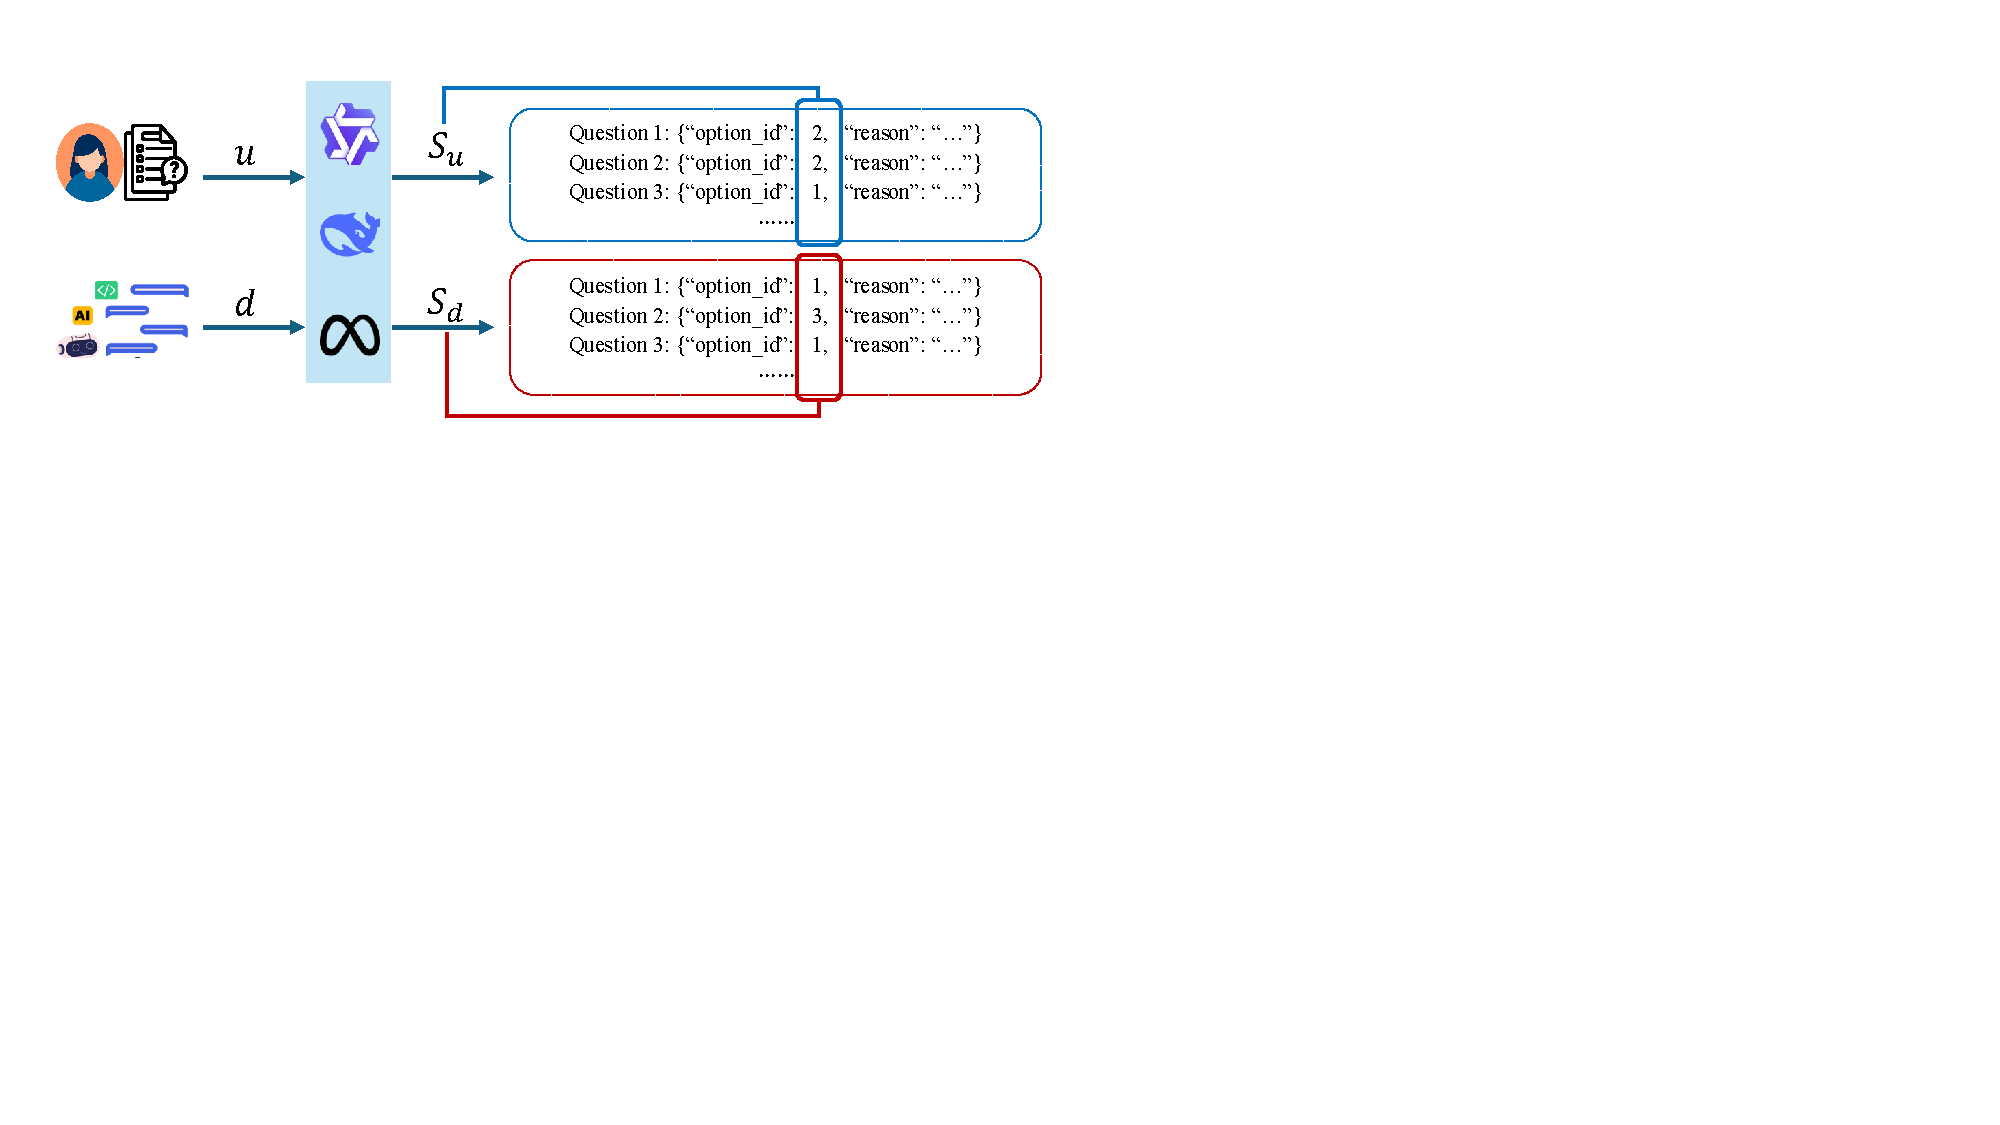
\includegraphics[trim=0.8cm 12cm 15cm 1.2cm,clip=true,width=0.7\textwidth]{figures/ModelEvaluation_new.pdf}
    \caption{Model querying workflow with key components. Here, $u$ denotes a user profile and $d$ a synthetic dialogue. Each response line represents the model's answer to a values question, including both the selected \texttt{option\_id} $s$ and a justification for the choice.}
    \label{fig:querying_model_workflow}
\end{center}
\end{figure}

To assess behavioral adaptation, we partition users and dialogues into demographic groups $g$ (by age, education, occupation, socioeconomic status, continent, immigration status). Each group is represented by a prototype vector $S_g$, where $s^j_g$ is the centroid of responses to question $q_j$. We measure inter-group divergence using normalized $L_1$ distance \citep{gowersdistance}:
\[
L_1(S_g, S_{g'}) = \sum_{j=1}^{m}
\left| \frac{s^j_g - s^j_{g'}}{\,h_j - \ell_j\,} \right|
\]
where $[\ell_j, h_j]$ is the ordinal range for question $q_j$. The baseline is the average distance from each group prototype to the global centroid.

\paratitle{Human Alignment Metric.}
\label{sec:alignment}

We frame alignment as a prediction task in which models predict individual human value responses conditioned on sociodemographic context. Let $\mathcal{H}_U = \{ H_u \}_{u \in U}$ denote the ground-truth human response vectors. In \texttt{BA\_user}, model predictions are given by the profile-conditioned response vectors $S_u$; in \texttt{BA\_dialogue}, predictions are given by the dialogue-conditioned response vectors $S_d$, which reflect the sociodemographic attributes of the underlying user inferred from the dialogue. We measure \emph{Value Alignment Accuracy} (VAA) as the average Pearson correlation \citep{freedman2007statistics} between model-predicted vectors and the corresponding human-reported vectors across users. Higher VAA indicates stronger alignment with empirically observed human value patterns and complements our preservation metrics, which assess \emph{how} alignment is achieved.

\begin{table}[H]
\centering
\small
\begin{tabular}{l|l|l}
\toprule
    \textbf{Metric Category} &  \textbf{Formula}  & \textbf{Baseline / Target} \\
    \midrule
    \multicolumn{3}{l}{\textit{Group-Level Behavioral Adaptation}} \\
    \midrule
    \texttt{Group Divergence}\  &
    $L_1(S_g, S_{g'}), \quad g, g' \subseteq U \text{ or } D$  &
    $\frac{1}{|G|} \sum_{g=1}^{|G|}   L_1(S_g, S_{\text{global}})$
    \\
    \midrule
    \multicolumn{3}{l}{\textit{Human Alignment (Section~\ref{sec:alignment})}} \\
    \midrule
    \texttt{VAA}\  &
    $\frac{1}{|U|} \sum_{u \in U} \rho(S_u^{\text{model}}, H_u)$ &
    Target: $> 0.5$
    \\
    \midrule
    \multicolumn{3}{l}{\textit{Individual Preservation (Section~\ref{sec:individual_preservation_metrics})}} \\
    \midrule
    \texttt{Homogenization}\  &
    $\frac{1}{|U|} \sum_{u \in U} \mathbb{I}\left( \|S_u^{\text{human}} - S_g^{\text{human}}\|_2 > \|S_u^{\text{model}} - S_g^{\text{human}}\|_2 \right)$ &
    Target: $< 30\%$
    \\
    \midrule
    \texttt{Centroid Pull}\  &
    $\frac{1}{|U|} \sum_{u \in U} \frac{(S_u^{\text{model}} - S_u^{\text{human}}) \cdot (S_g^{\text{human}} - S_u^{\text{human}})}{\|S_g^{\text{human}} - S_u^{\text{human}}\|_2}$ &
    Target: $\approx 0$
    \\
    \midrule
    \texttt{Variance Ratio}\  &
    $\frac{\text{std}(S_g^{\text{model}})}{\text{std}(S_g^{\text{human}})}$ &
    Target: $[0.8, 1.2]$
    \\
    \midrule
    \texttt{Group Bias Amp.}\  &
    $\frac{L_1(S_g^{\text{model}}, S_{g'}^{\text{model}})}{L_1(S_g^{\text{human}}, S_{g'}^{\text{human}})}$ &
    Target: $< 1.2$
    \\
    \midrule
    \multicolumn{3}{l}{\textit{Cross-Format Consistency (Section~\ref{sec:consistency_distance})}} \\
    \midrule
    \texttt{Group Pattern}\  &
    $\rho\left( \{L_1(S_g^U, S_{g'}^U)\}, \{L_1(S_g^D, S_{g'}^D)\} \right)$ &
    Target: $> 0.7$
    \\
    \midrule
    \texttt{Metric Stability}\  &
    $\left| M^{\texttt{user}} - M^{\texttt{dialogue}} \right| / M^{\texttt{user}}$ &
    Target: $< 0.2$
    \\
    \midrule
    \texttt{Response Match}\  &
    $ \frac{1}{|U|} \sum_{i=1}^{|U|}
      L_1\left(S_u, S_d \right) \Big/ \text{baseline}$&
    Target: $< 0.9$
    \\

\bottomrule

\end{tabular}
\caption{Evaluation metrics organized by category. \textbf{Group-Level Adaptation}: measures inter-group divergence in model responses. \textbf{Human Alignment}: \texttt{VAA} (Value Alignment Accuracy) measures Pearson correlation between model and human response vectors, indicating how well models capture genuine human value patterns. \textbf{Individual Preservation}: measures whether models preserve individual uniqueness, including \texttt{Homogenization} (percentage pulled toward centroids), \texttt{Centroid Pull} (directional movement), \texttt{Variance Ratio} (diversity preservation), \texttt{Group Bias Amp.} (amplification vs. humans). \textbf{Cross-Format Consistency}: compares metrics across formats, including \texttt{Group Pattern} (Spearman $\rho$), \texttt{Metric Stability}, \texttt{Response Match}. All metrics except \texttt{Response Match} are computed separately per format.}
\label{tab:measure_forms}
\end{table}

\subsection{Individual Preservation Metrics}
\label{sec:individual_preservation_metrics}

Adaptation metrics assess whether models respond to demographics but do not reveal \textit{how} alignment is achieved. A model might attain high VAA either through genuine personalization or by collapsing individuals toward demographic centroids. To distinguish these mechanisms, we introduce individual preservation metrics.

\paratitle{Homogenization Rate (\textit{pct\_toward\_centroid}):}
The percentage of individuals whose model responses shift toward their demographic group centroid $S_g^{\text{human}}$. For each individual $u$ in group $g$, we measure whether the model output $S_u^{\text{model}}$ is closer to the human group centroid $S_g^{\text{human}}$ than the human baseline $S_u^{\text{human}}$. Lower values indicate better preservation of individual uniqueness. We target a rate $< 30\%$, meaning at least 70\% of individuals maintain distinct positions relative to their demographic group.

\paratitle{Centroid Pull Magnitude (\textit{mean\_delta}):}
The average directional movement of individuals toward group centroids, measured as the projection of the displacement vector $(S_u^{\text{model}} - S_u^{\text{human}})$ onto the normalized direction toward the human group centroid
\[
\hat{d}_u = \frac{S_g^{\text{human}} - S_u^{\text{human}}}{\left\| S_g^{\text{human}} - S_u^{\text{human}} \right\|}.
\]
Negative values indicate systematic pull toward demographic centroids, while values near zero indicate minimal homogenization. This metric captures not only whether individuals move, but whether they consistently move \textit{toward} group prototypes. Homogenization rate measures the prevalence of stereotype convergence, whereas centroid pull magnitude quantifies the directional strength of this convergence, enabling distinction between widespread mild drift and concentrated strong bias.

\paratitle{Within-Group Variance Preservation (\textit{std\_ratio}):}
The ratio of within-group standard deviation in model outputs to human baseline: $\text{std}(S_g^{\text{model}}) / \text{std}(S_g^{\text{human}})$. Healthy range: $[0.8, 1.2]$. Values below 0.8 indicate problematic variance collapse where the model suppresses individual diversity within demographic groups.


\paratitle{Group Bias Amplification (\textit{vs\_human\_ratio}):}
The ratio of demographic group differences in model outputs to human baselines. Computed as the ratio of inter-group distances: model distance divided by human distance. Values $< 1.0$ indicate bias reduction; values $> 1.2$ indicate concerning amplification where the model exaggerates group differences beyond human patterns.

\paratitle{Outlier Preservation Rate (\textit{retention\_rate}):}
The percentage of atypical individuals (outliers within demographic groups, defined as those beyond 1.5 IQR from group median) who remain atypical in model outputs. Target $> 0.7$. This metric captures whether models erase individuals who deviate from their demographic group's typical profile.

These metrics are computed across all three scenarios (\texttt{BA\_user}, \texttt{BA\_dialogue} Career, \texttt{BA\_dialogue} Investment) and six demographic attributes (age, education, occupation, socioeconomic status, continent, immigration status).

\subsection{Cross-Format Consistency Metrics}
\label{sec:consistency_distance}

Adaptation and preservation are evaluated within each input format independently. Consistency metrics synthesize across formats: do models maintain consistent adaptation and preservation properties when the same demographic information is presented via explicit user profiles versus inferred from dialogue history? This reveals whether behavioral patterns reflect stable demographic understanding or are confounded by surface-level prompt variations.

\paratitle{Group-Level Consistency:}
We compare group divergence patterns between \texttt{BA\_user} and \texttt{BA\_dialogue} formats. For each demographic attribute, we compute the Spearman correlation $\rho$ between the vectors of pairwise inter-group distances in the two formats. High correlation ($\rho > 0.7$) indicates that the model preserves relative group relationships regardless of how demographic attributes are presented. For example, if age groups ``<30'' and ``>60'' show the largest divergence in \texttt{BA\_user}, a consistent model should exhibit similar relative divergence in \texttt{BA\_dialogue}.

\paratitle{Individual-Level Consistency:}
We compare the individual preservation metrics (homogenization rate, centroid pull, variance ratio) across formats. A model exhibits strong cross-format consistency if these metrics show similar values in \texttt{BA\_user} and \texttt{BA\_dialogue} scenarios. Large discrepancies indicate that preservation properties are context-dependent rather than reflecting stable model behavior.

\paratitle{Response-Level Consistency:}
For matched user profile--dialogue pairs $(u, d)$ representing the same individual, we compute the normalized $L_1$ distance between response vectors $S_u^{\text{model}}$ and $S_d^{\text{model}}$, normalized by a baseline from mismatched pairs. Lower ratios indicate that the model produces more similar responses when processing equivalent demographic information in different formats. Detailed response-level results are provided in Appendix~\ref{appendix:response_consistency}.

Table~\ref{tab:measure_forms} summarizes all evaluation metrics with their formulas and target values.

\subsection{Experiment Setting}

Following the workflow in Figure~\ref{fig:querying_model_workflow}, we evaluate several open-source LLMs---including the \textit{Qwen2.5} and \textit{Llama-3.1} families, \textit{DeepSeek-V3}, and the reasoning-augmented \textit{QwQ-32B} \citep{qwen2025qwen25technicalreport, dubey2024llama3herdmodels, deepseekai2025deepseekv3technicalreport}---to generate $\mathcal{S}_U$ and $\mathcal{S}_D$. We employ XGrammar \citep{dong2025xgrammar} to serialize model outputs into JSON, ensuring reliable structured extraction. Notably, \textit{QwQ-32B} is prompted to produce unconstrained reasoning alongside its structured response.

%======================================
\section{Evaluation Outcomes}
\label{sec:evaluation_outcomes}
%======================================

\begin{figure}[H]
\begin{center}
    \setlength{\tabcolsep}{6pt}
    \begin{tabular}{@{}c c c@{}}
      \multicolumn{3}{c}{%
        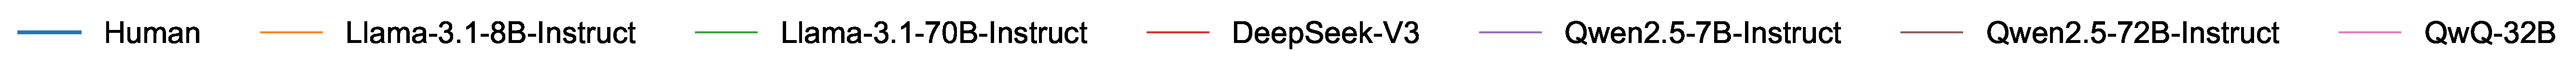
\includegraphics[width=0.95\columnwidth]{./figures/wvs_model_behavior_figures/radar_legend.pdf}%
      }\\
      \addlinespace[2pt]
      \toprule
      \multicolumn{3}{l}{\textbf{Grouped by Age}}\\[-0.4ex]
      \cmidrule(l){1-3}
      \subfloat[BA\_user]{%
        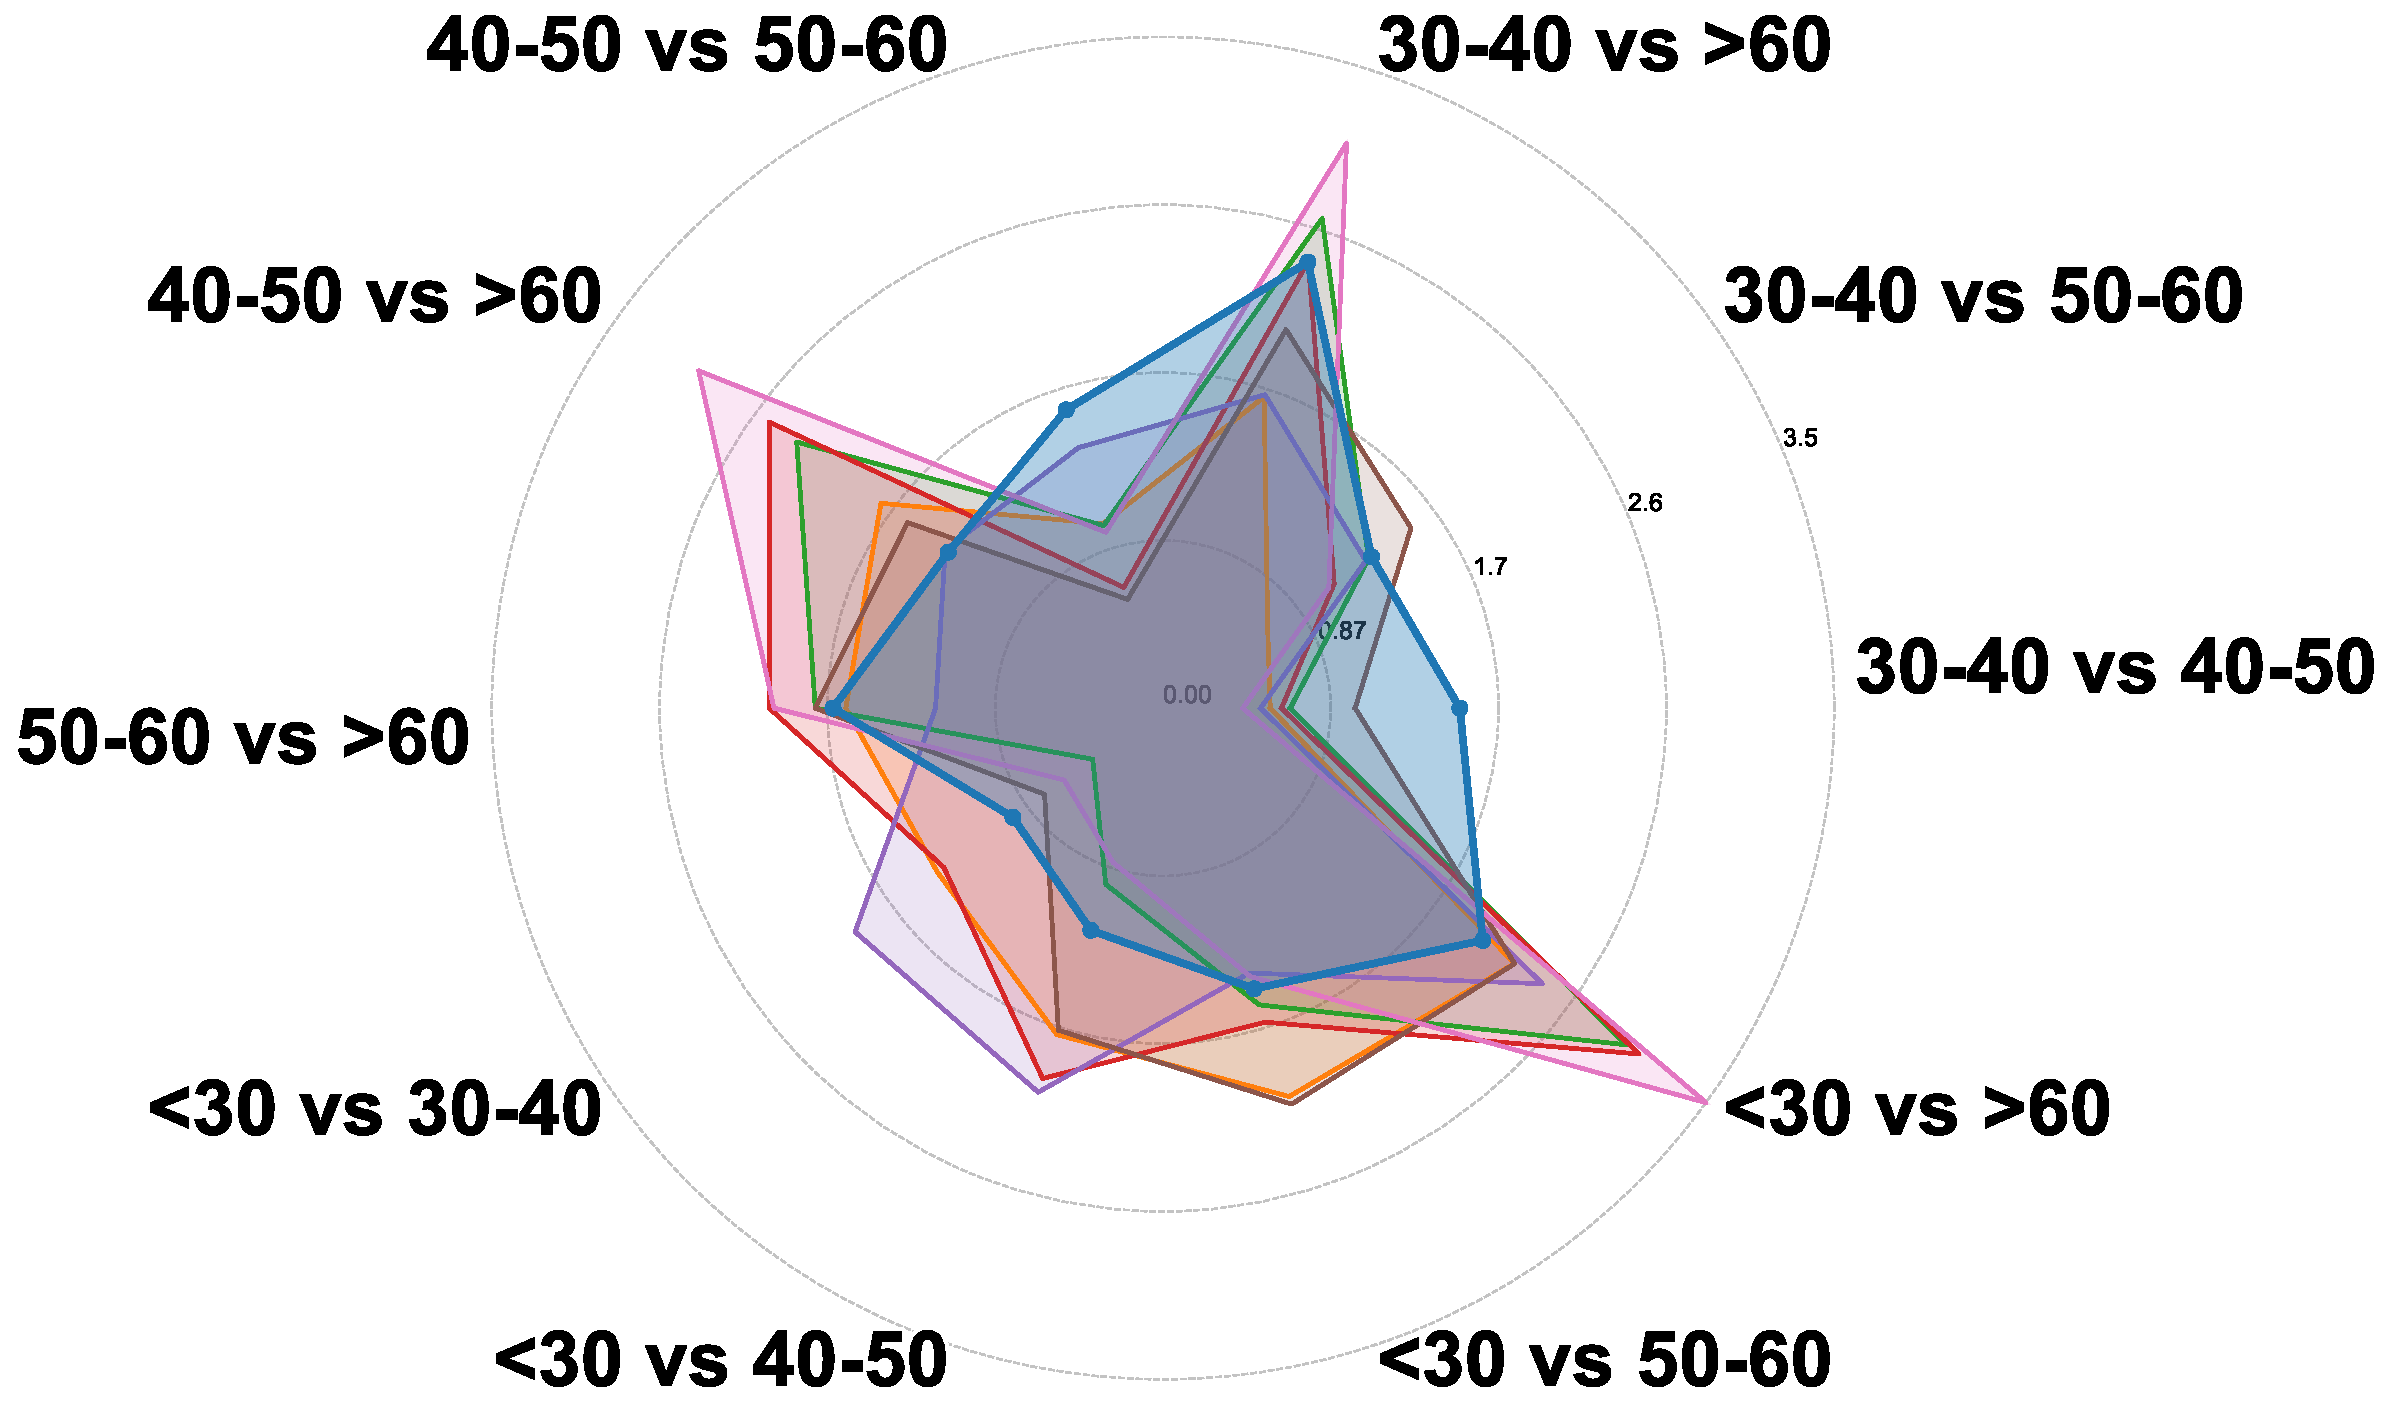
\includegraphics[width=0.31\columnwidth]{./figures/wvs_model_behavior_figures/ba_user/ba_user_age_radar.pdf}%
      }
      &
      \subfloat[BA\_dialogue (Career)]{%
        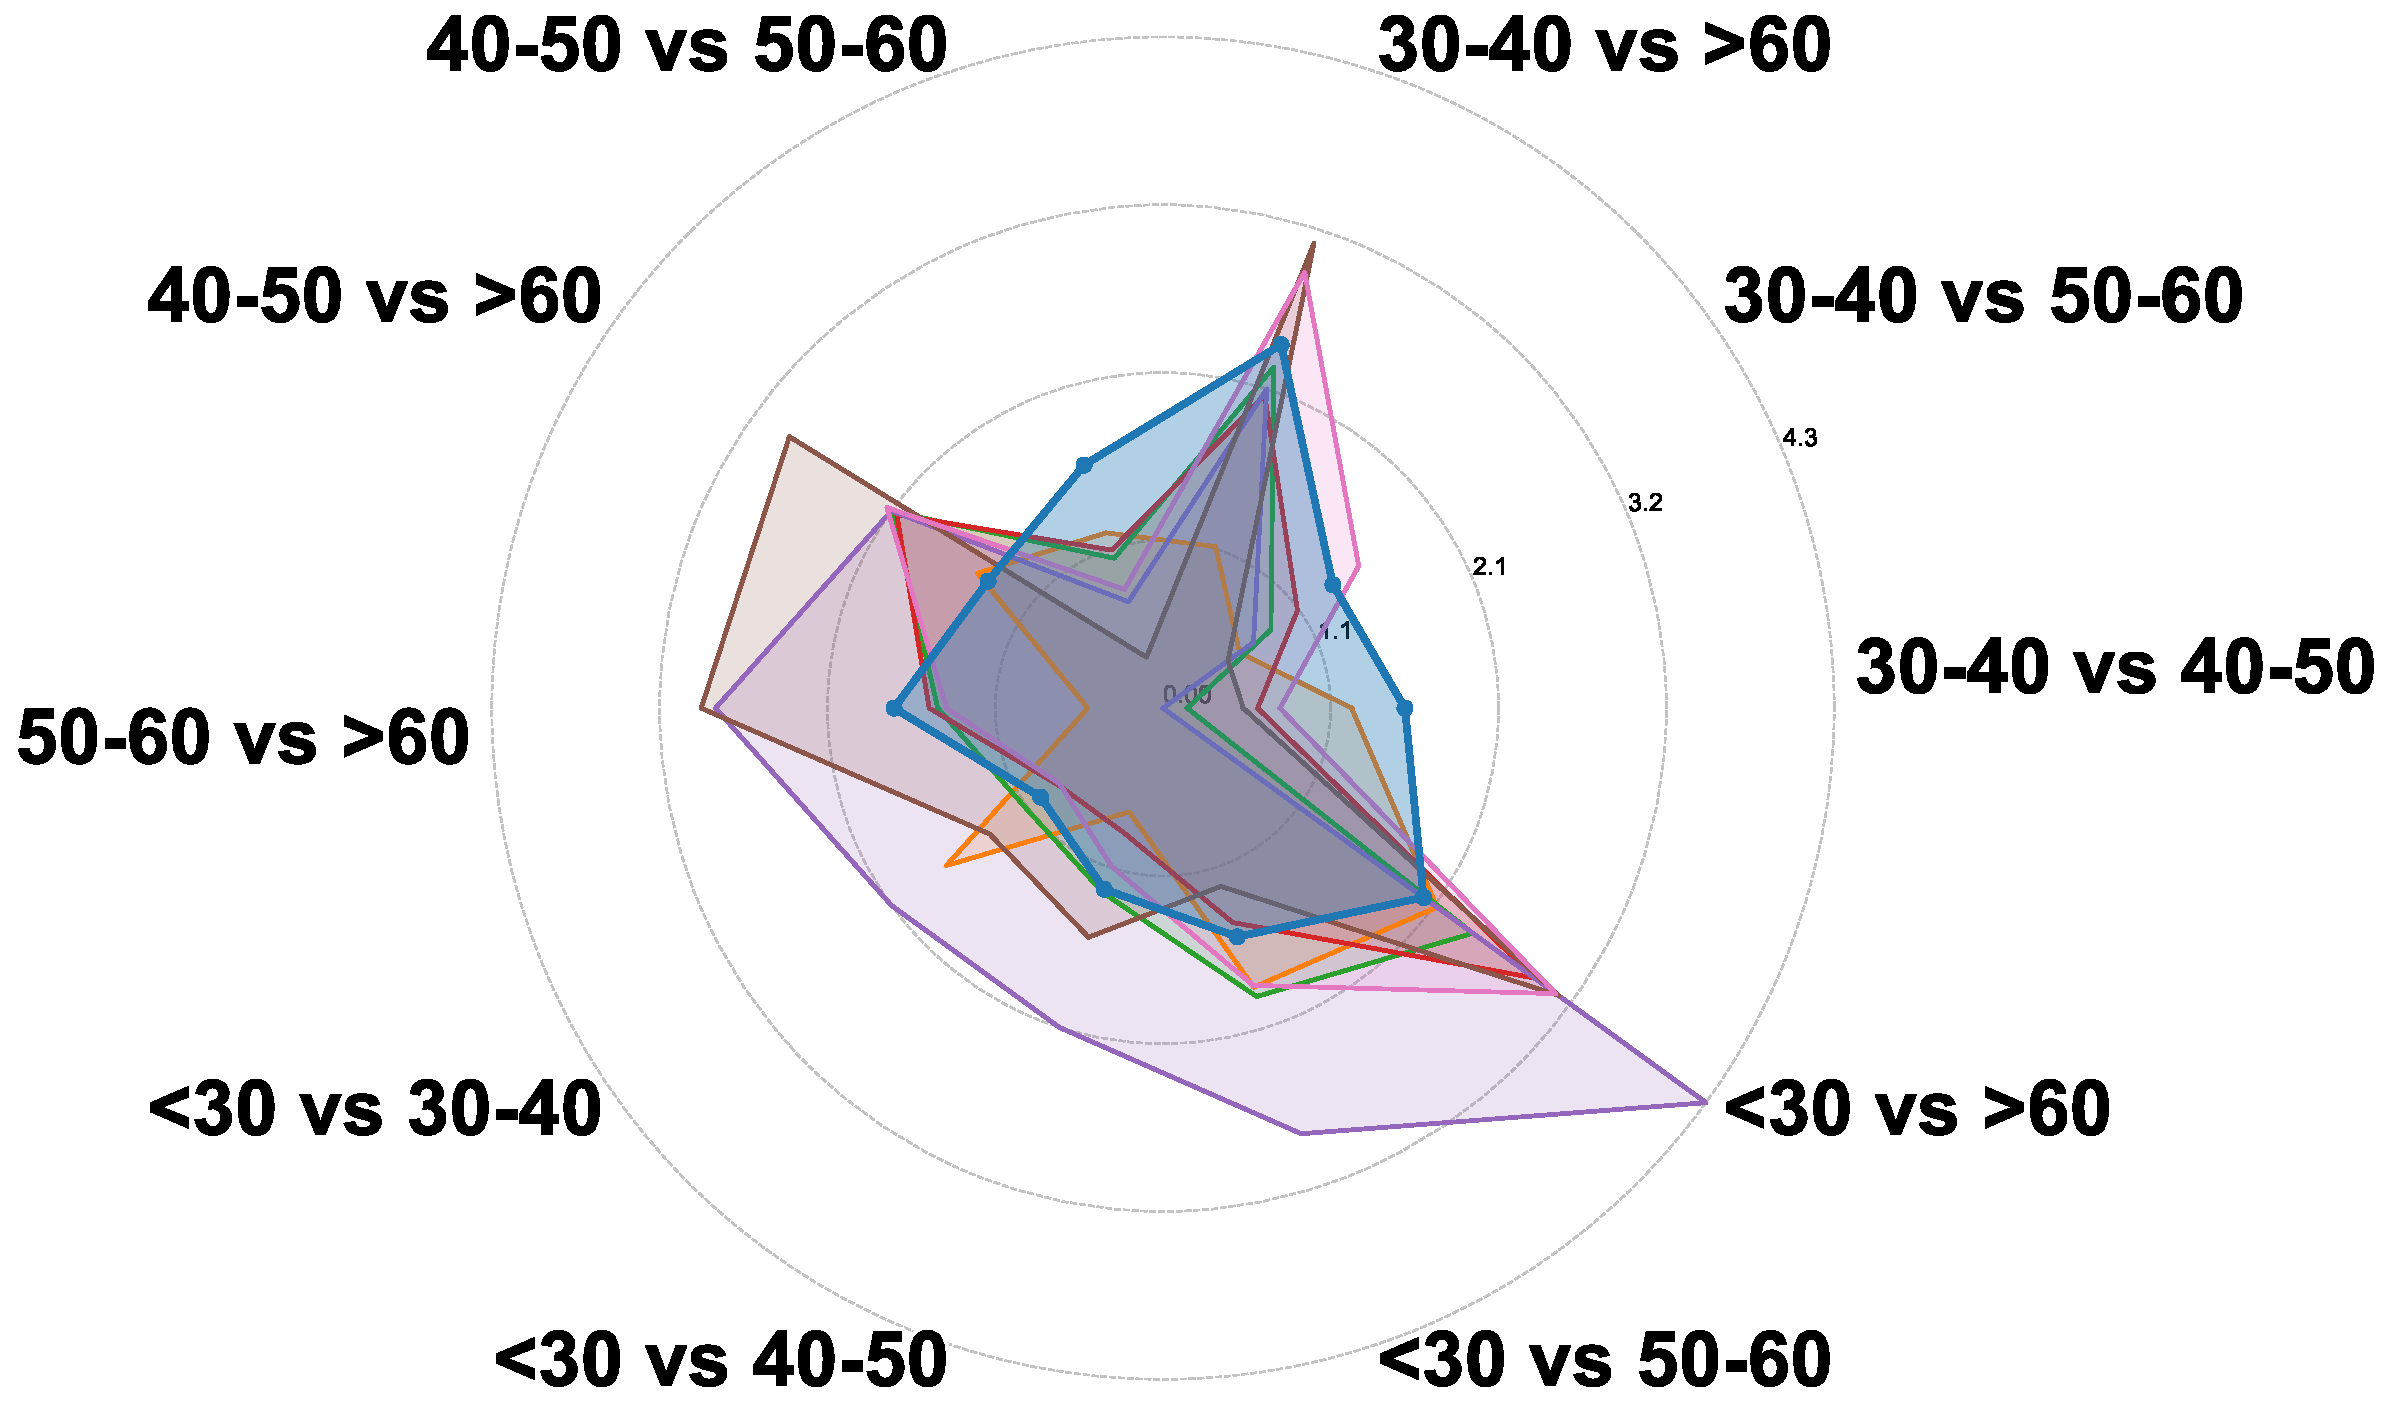
\includegraphics[width=0.31\columnwidth]{./figures/wvs_model_behavior_figures/ba_dialogue_career/ba_dialogue_career_age_radar.pdf}%
      }
      &
      \subfloat[BA\_dialogue (Investment)]{%
        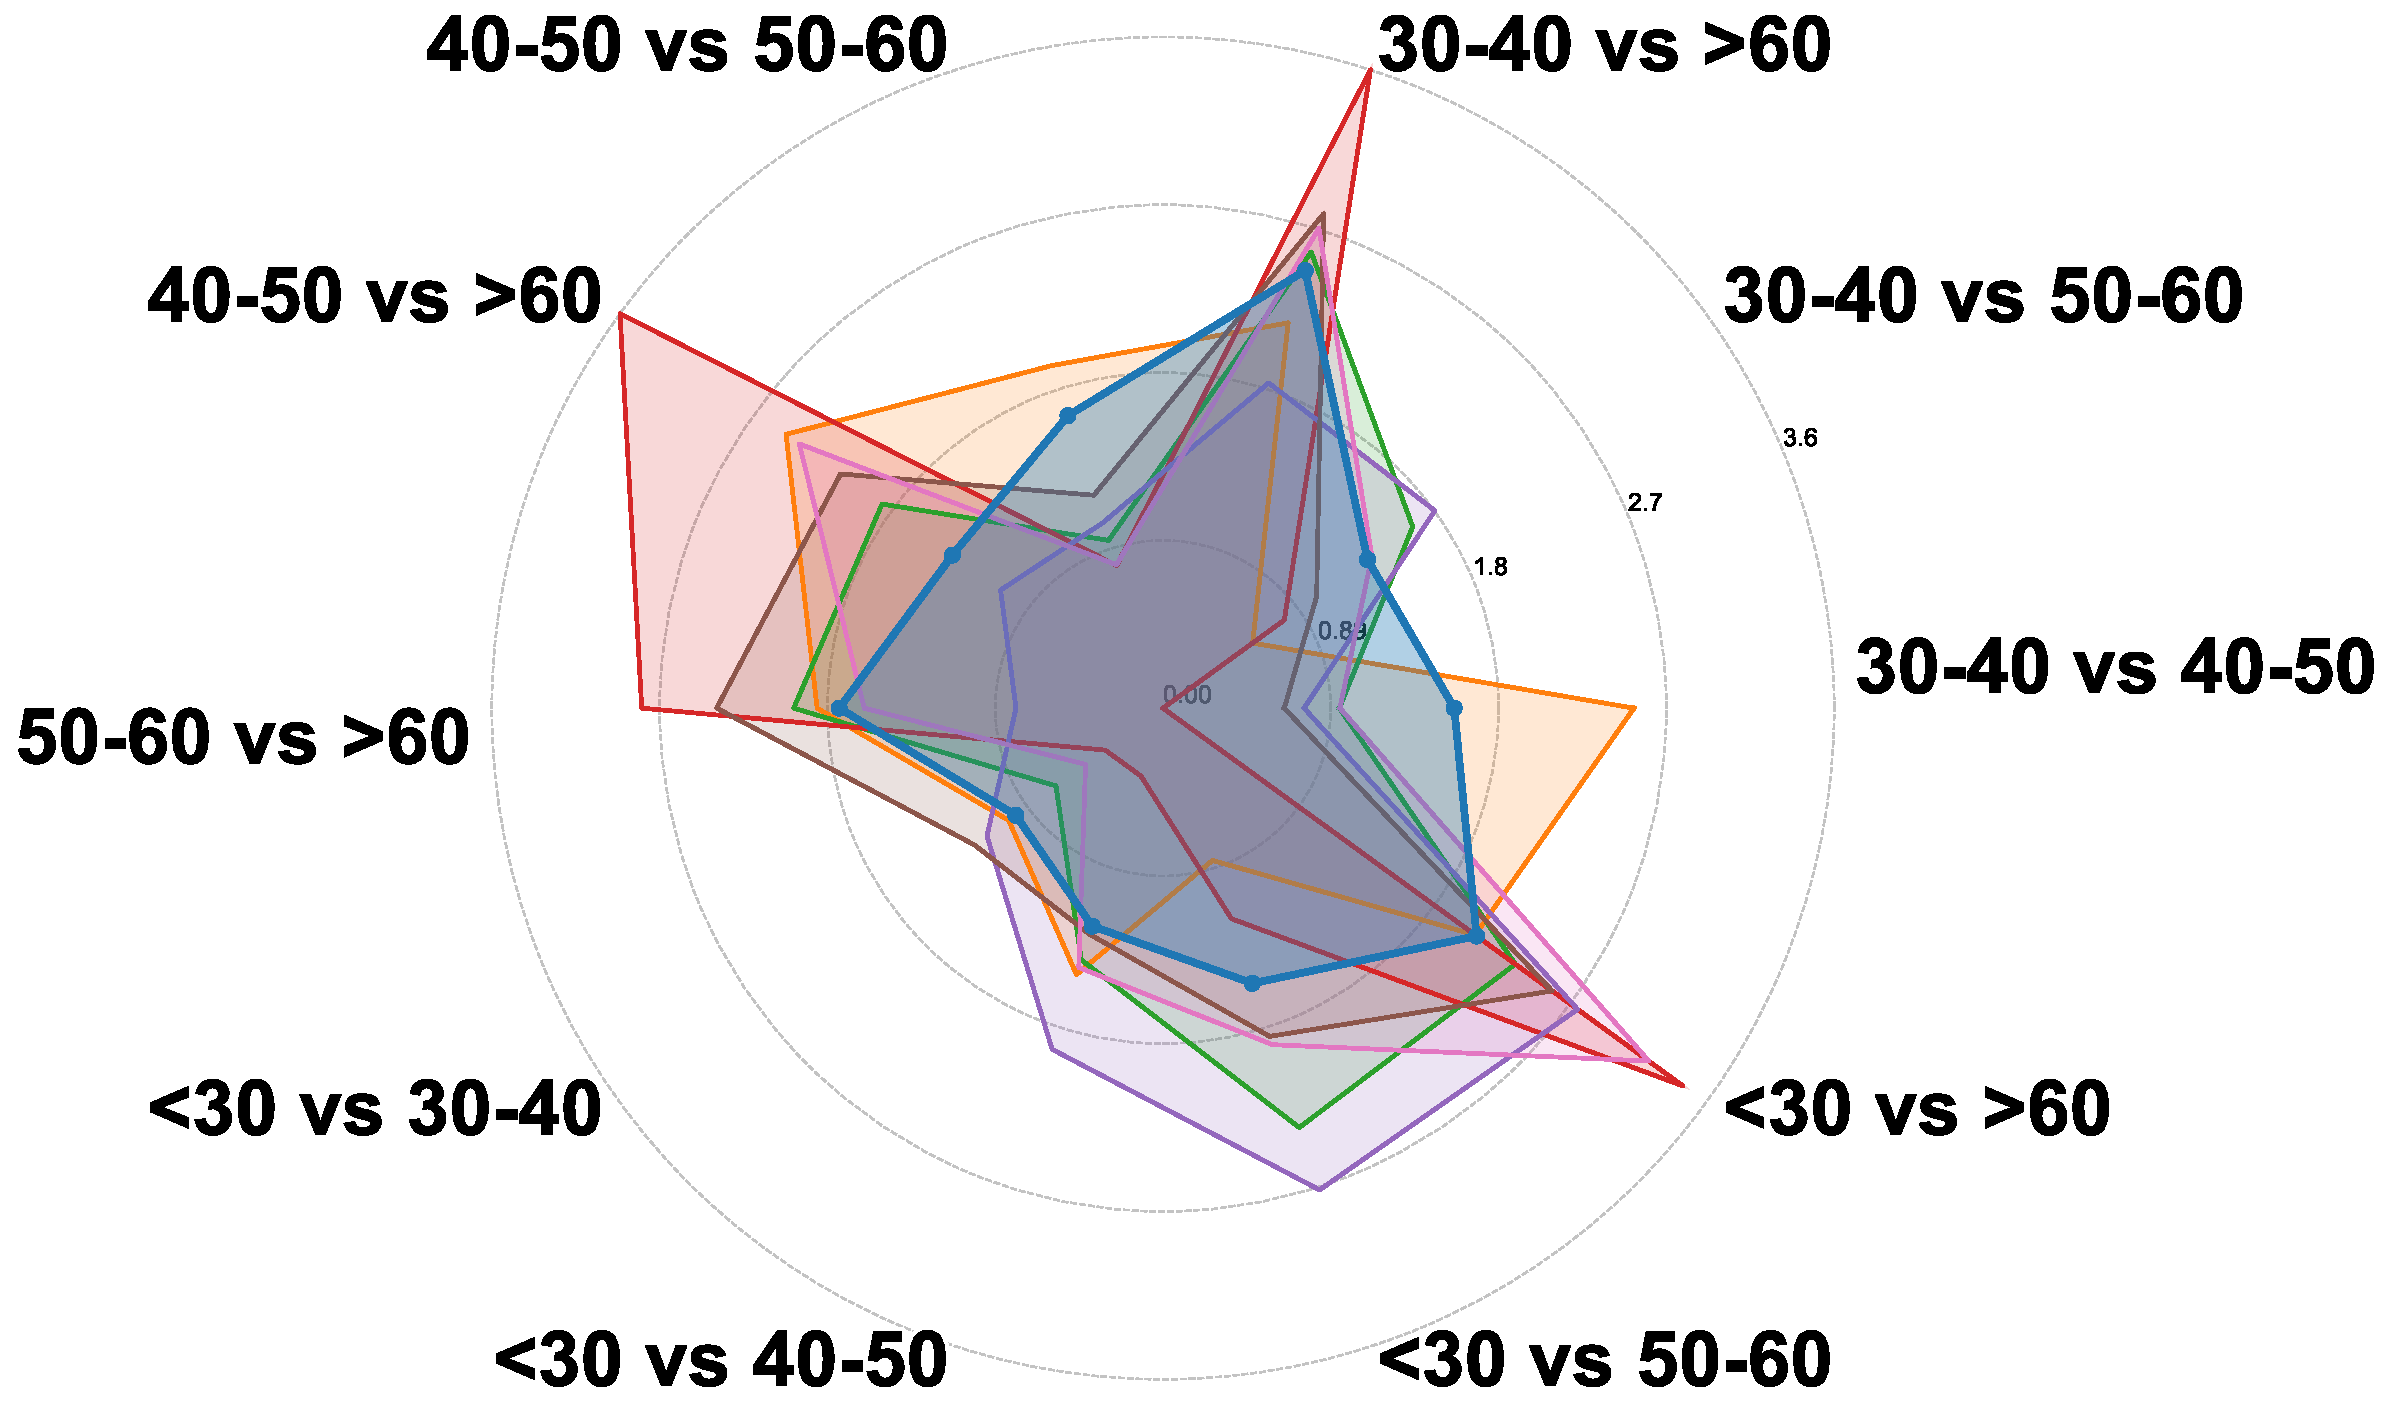
\includegraphics[width=0.31\columnwidth]{./figures/wvs_model_behavior_figures/ba_dialogue_investment/ba_dialogue_investment_age_radar.pdf}%
      }
      \\[0.6ex]
      \addlinespace[2pt]
      \toprule
      \multicolumn{3}{l}{\textbf{Grouped by Education}}\\[-0.4ex]
      \cmidrule(l){1-3}
      \subfloat[BA\_user]{%
        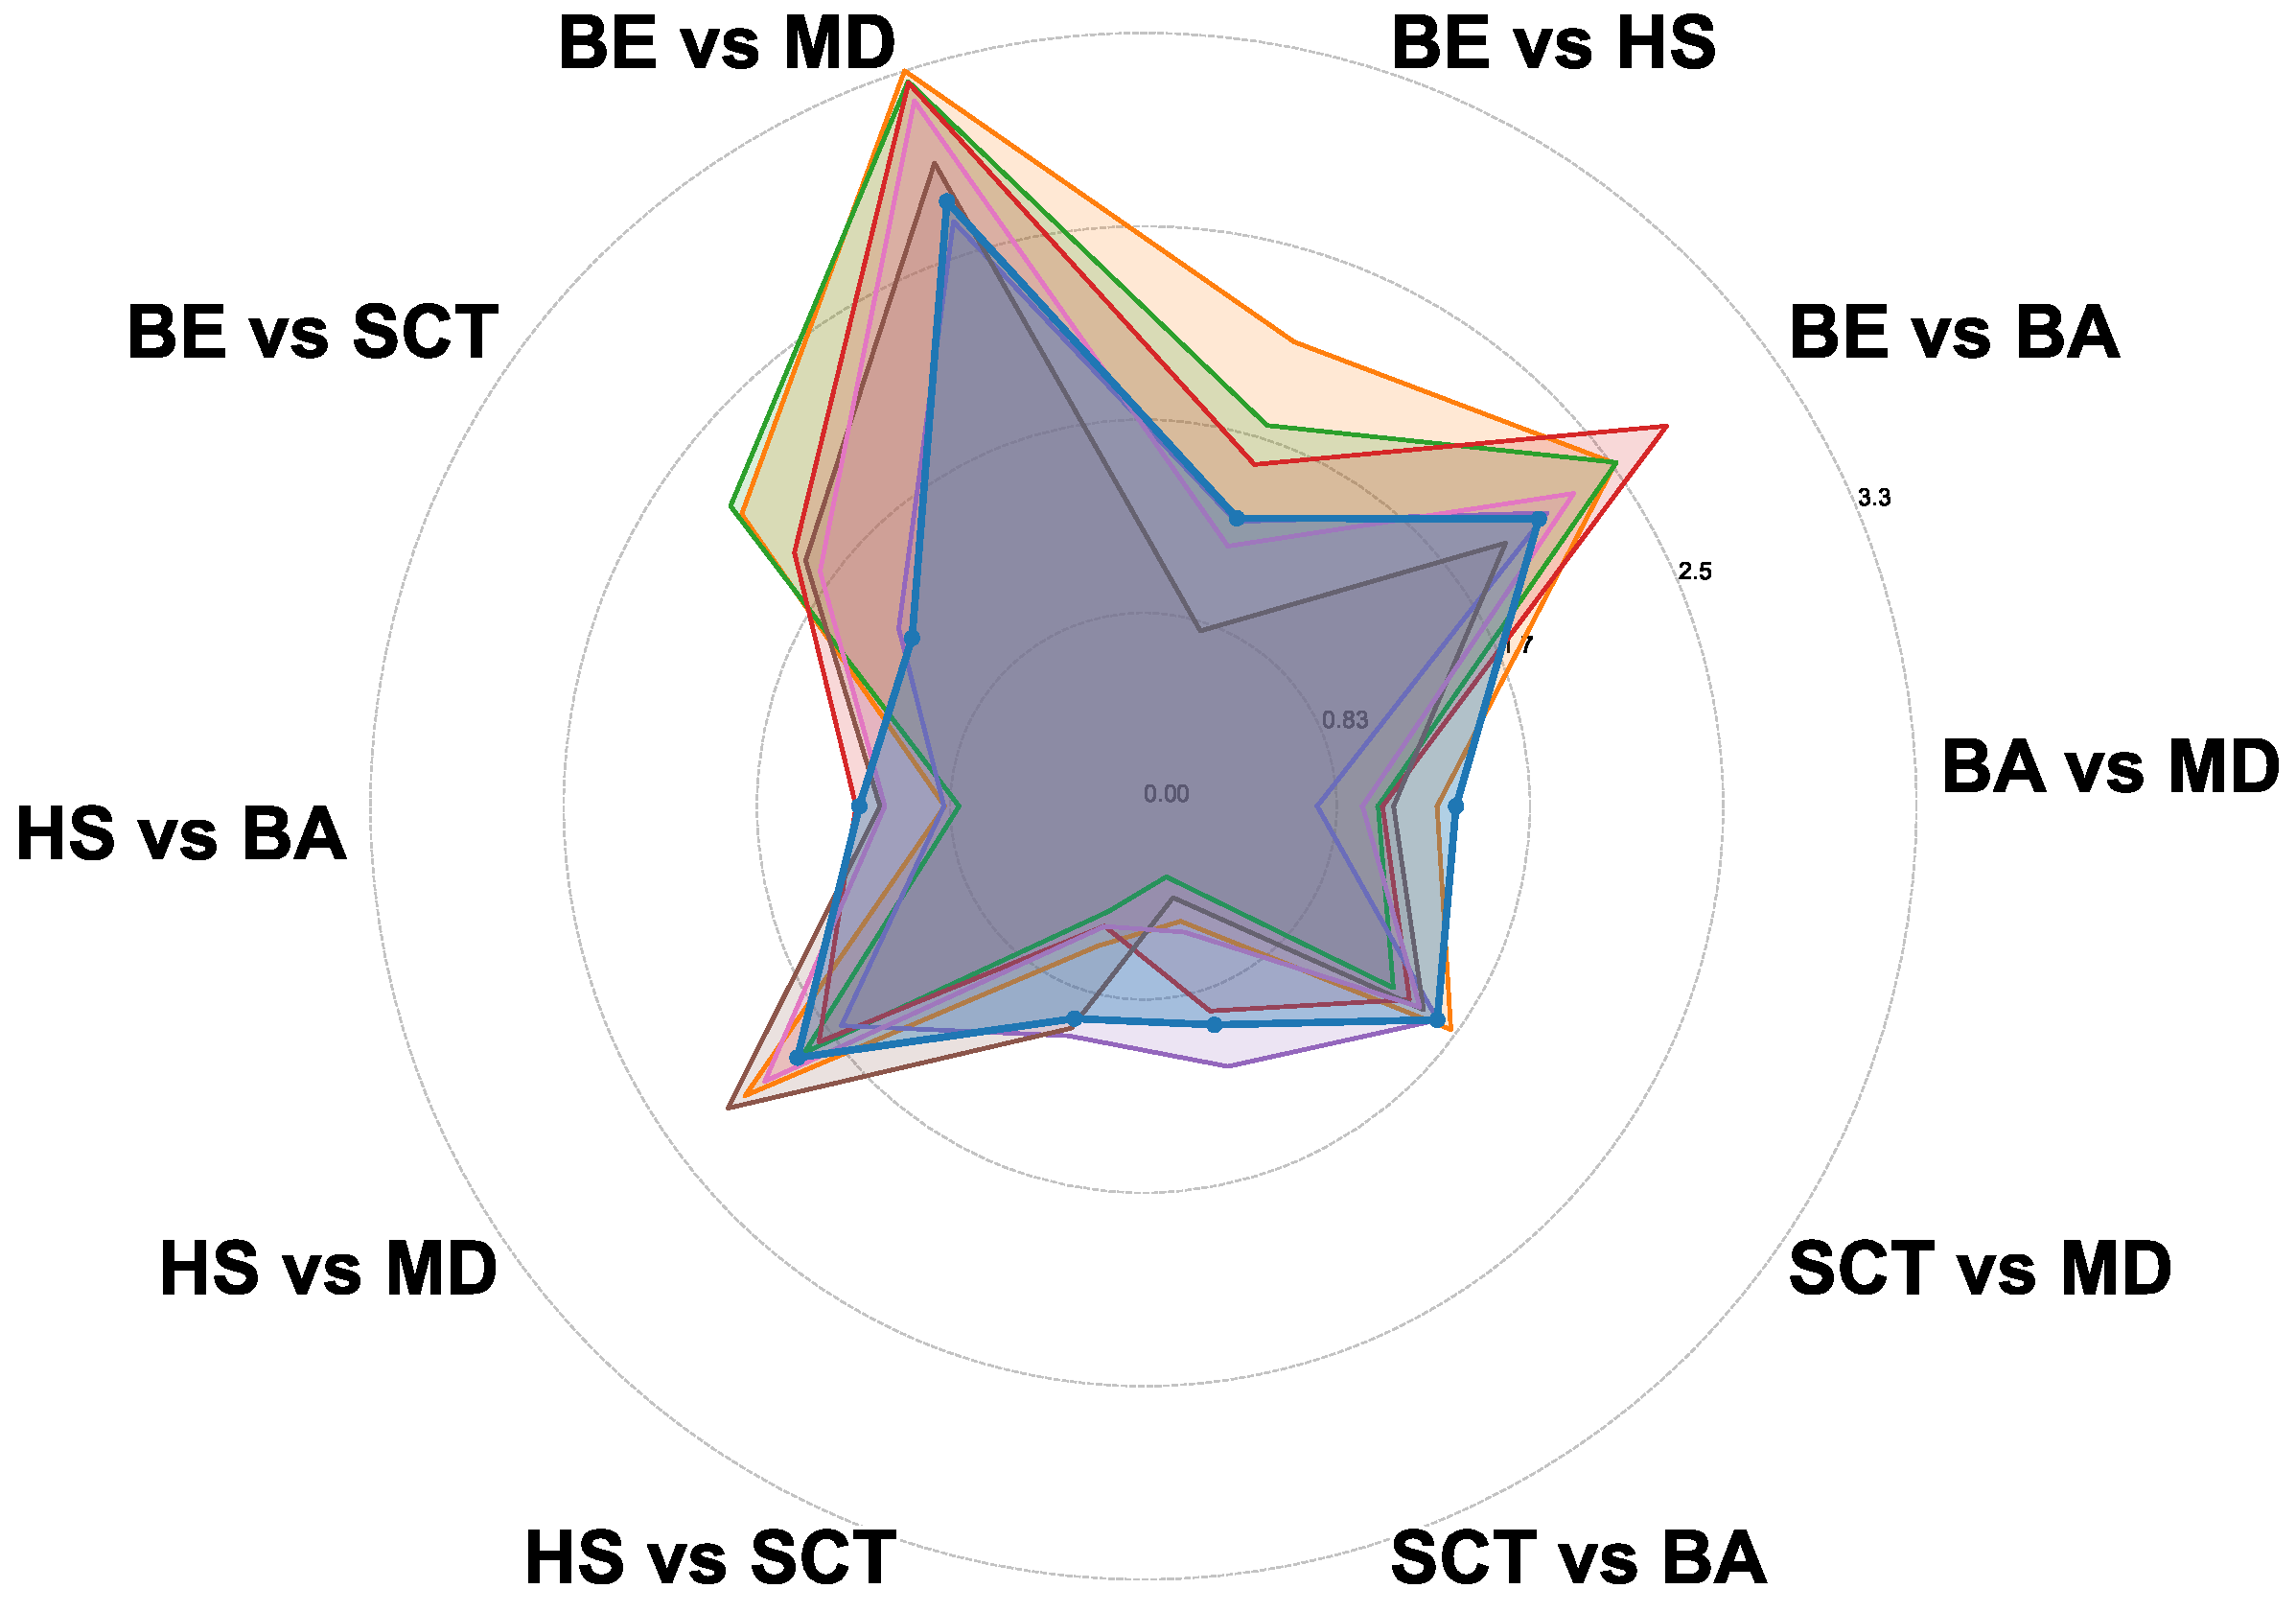
\includegraphics[width=0.31\columnwidth]{./figures/wvs_model_behavior_figures/ba_user/ba_user_education_radar.pdf}%
      }
      &
      \subfloat[BA\_dialogue (Career)]{%
        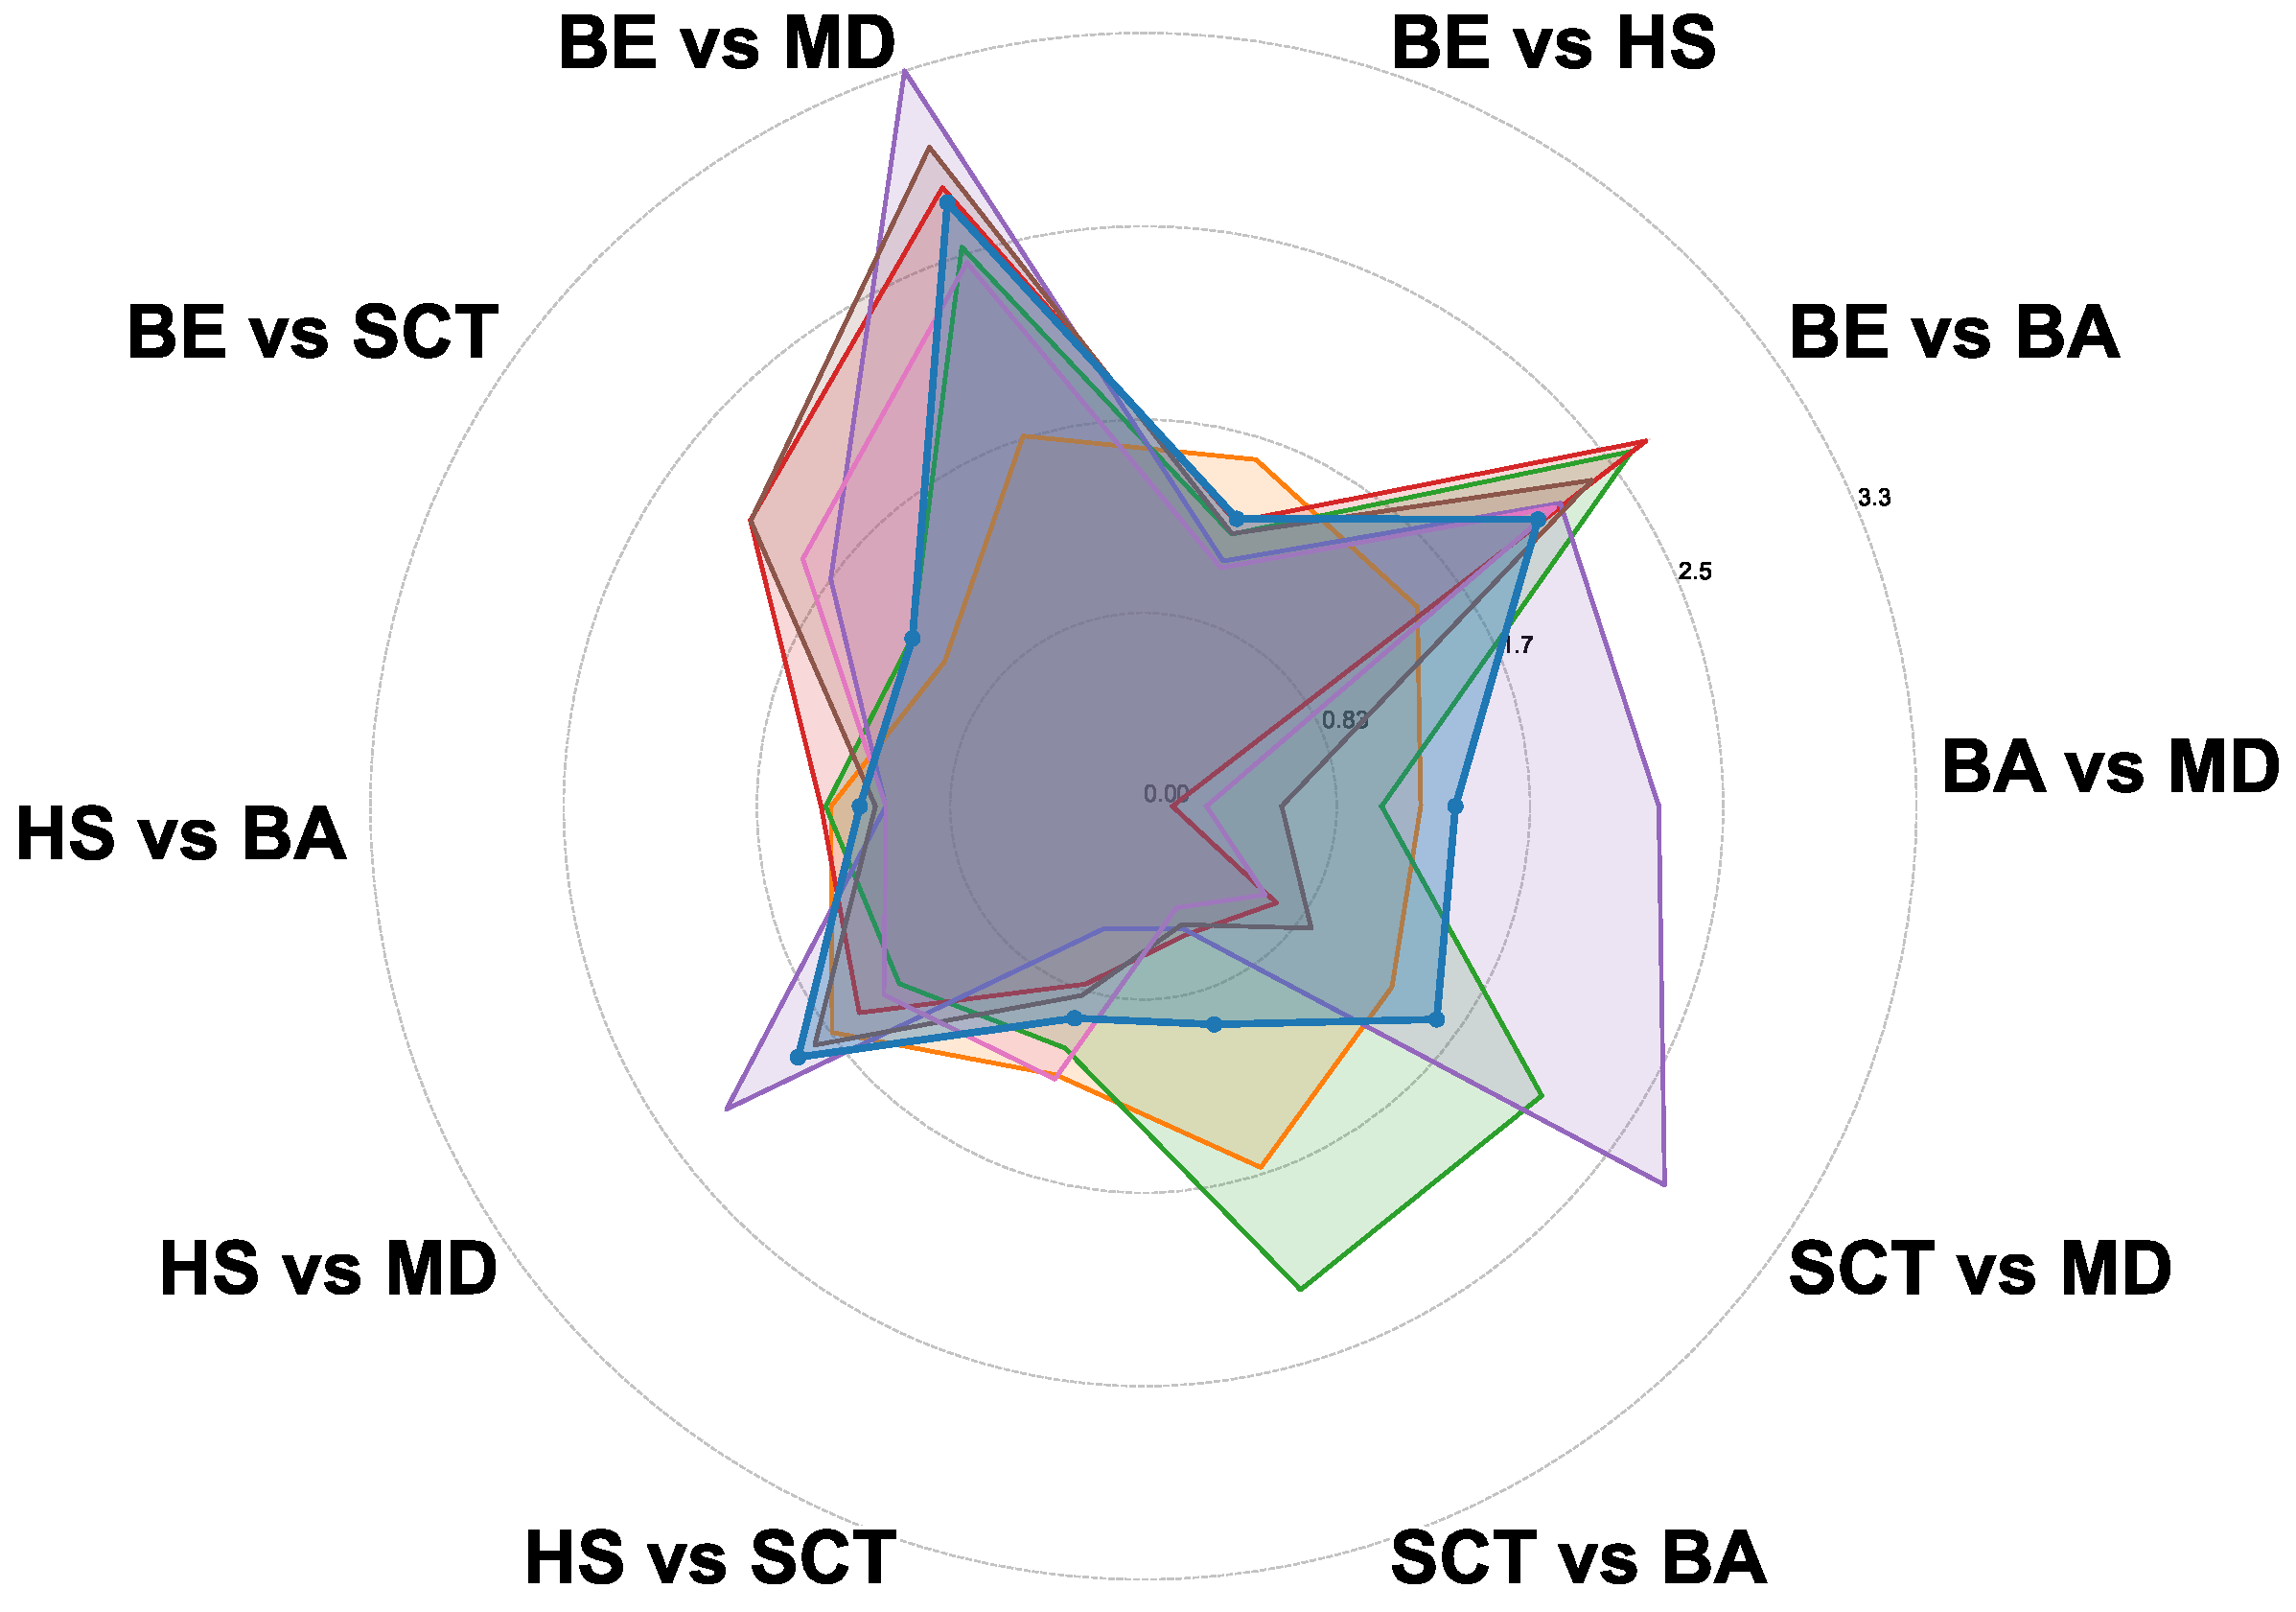
\includegraphics[width=0.31\columnwidth]{./figures/wvs_model_behavior_figures/ba_dialogue_career/ba_dialogue_career_education_radar.pdf}%
      }
      &
      \subfloat[BA\_dialogue (Investment)]{%
        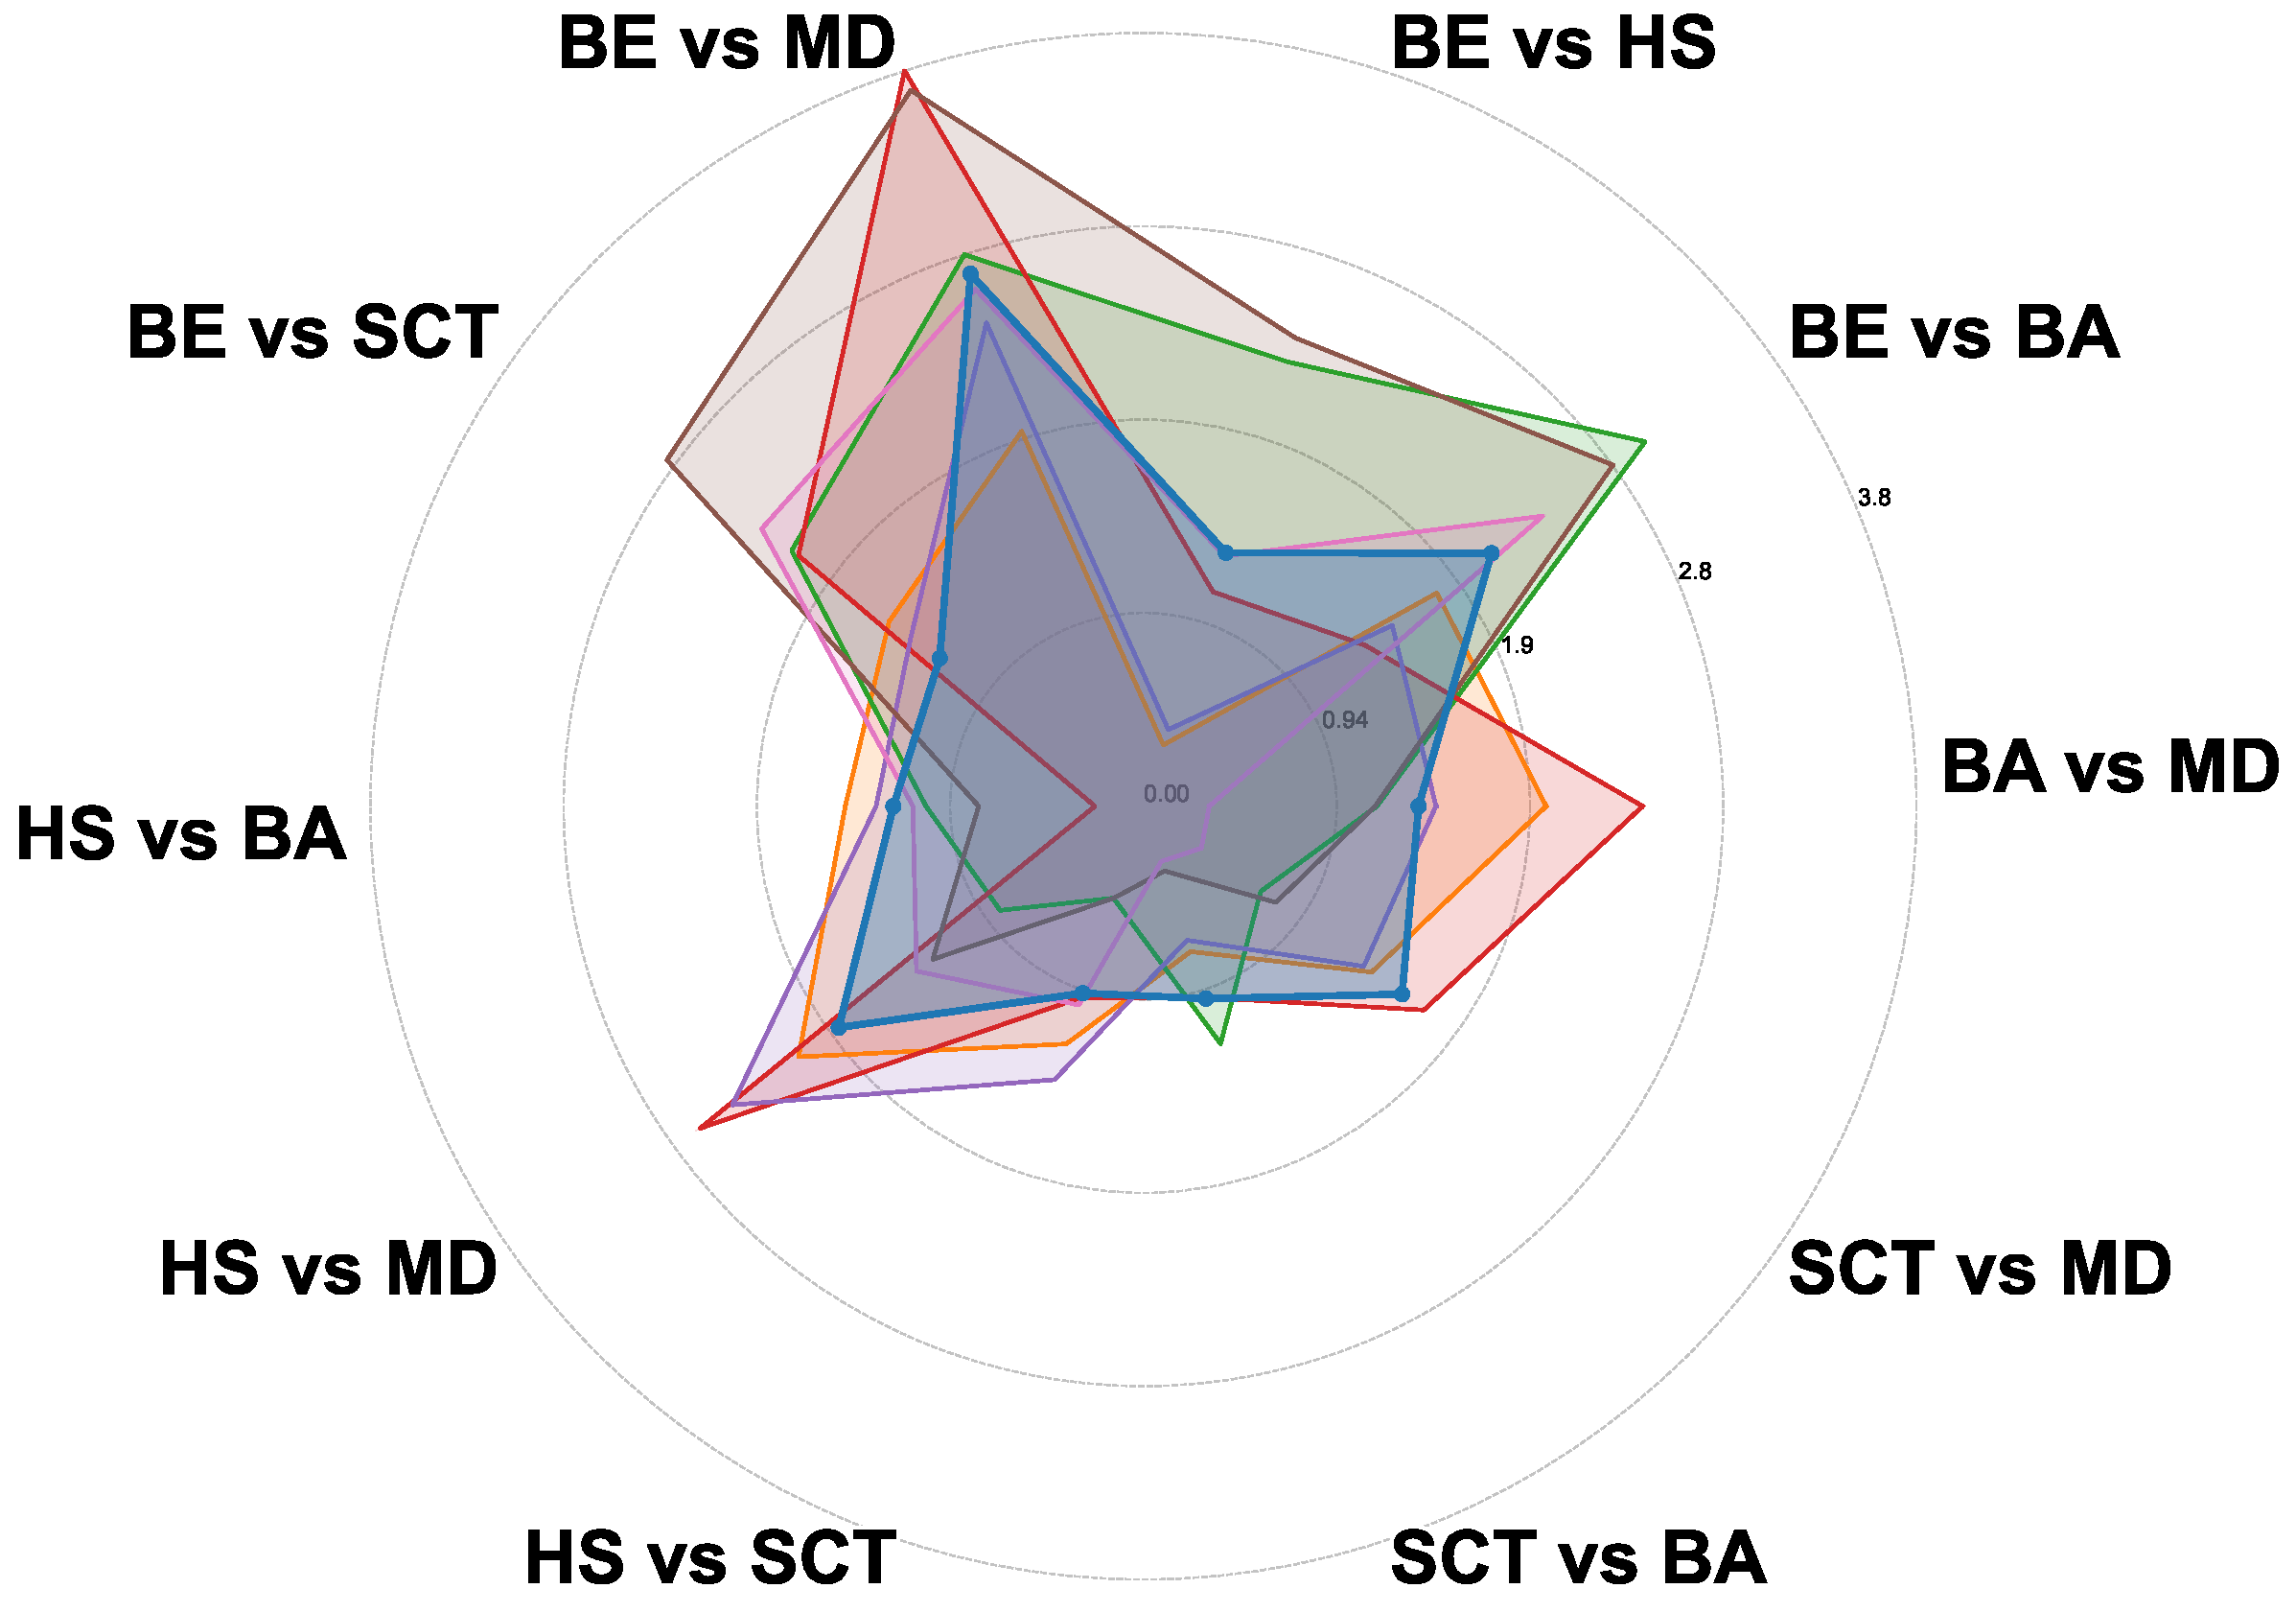
\includegraphics[width=0.31\columnwidth]{./figures/wvs_model_behavior_figures/ba_dialogue_investment/ba_dialogue_investment_education_radar.pdf}%
      }
      \\[0.6ex]
    \bottomrule
    \end{tabular}
\caption{Illustration of \texttt{BA\_user} and \texttt{BA\_dialogue} measurements. The first row compares groups by ``Age,'' and the second by ``Education Level.'' Most models demonstrate a positive correlation between computed distances and demographic differences. \emph{Abbreviations} --- Education: BE (Basic education), HS (High school \& equivalent), SCT (Short-cycle tertiary), BA (Bachelor), MD (Master's \& Doctoral).}
\label{fig:ba_evaluation_1}
\end{center}
\end{figure}

\begin{figure}[H]
\begin{center}
    \setlength{\tabcolsep}{6pt}
    \begin{tabular}{@{}c c c@{}}
      \multicolumn{3}{c}{%
        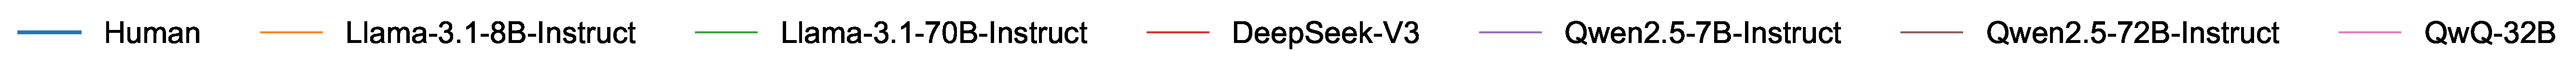
\includegraphics[width=0.95\columnwidth]{./figures/wvs_model_behavior_figures/radar_legend.pdf}%
      }\\
      \addlinespace[2pt]
      \toprule
      \multicolumn{3}{l}{\textbf{Grouped by Occupation Group}}\\[-0.4ex]
      \cmidrule(l){1-3}
      \subfloat[BA\_user]{%
        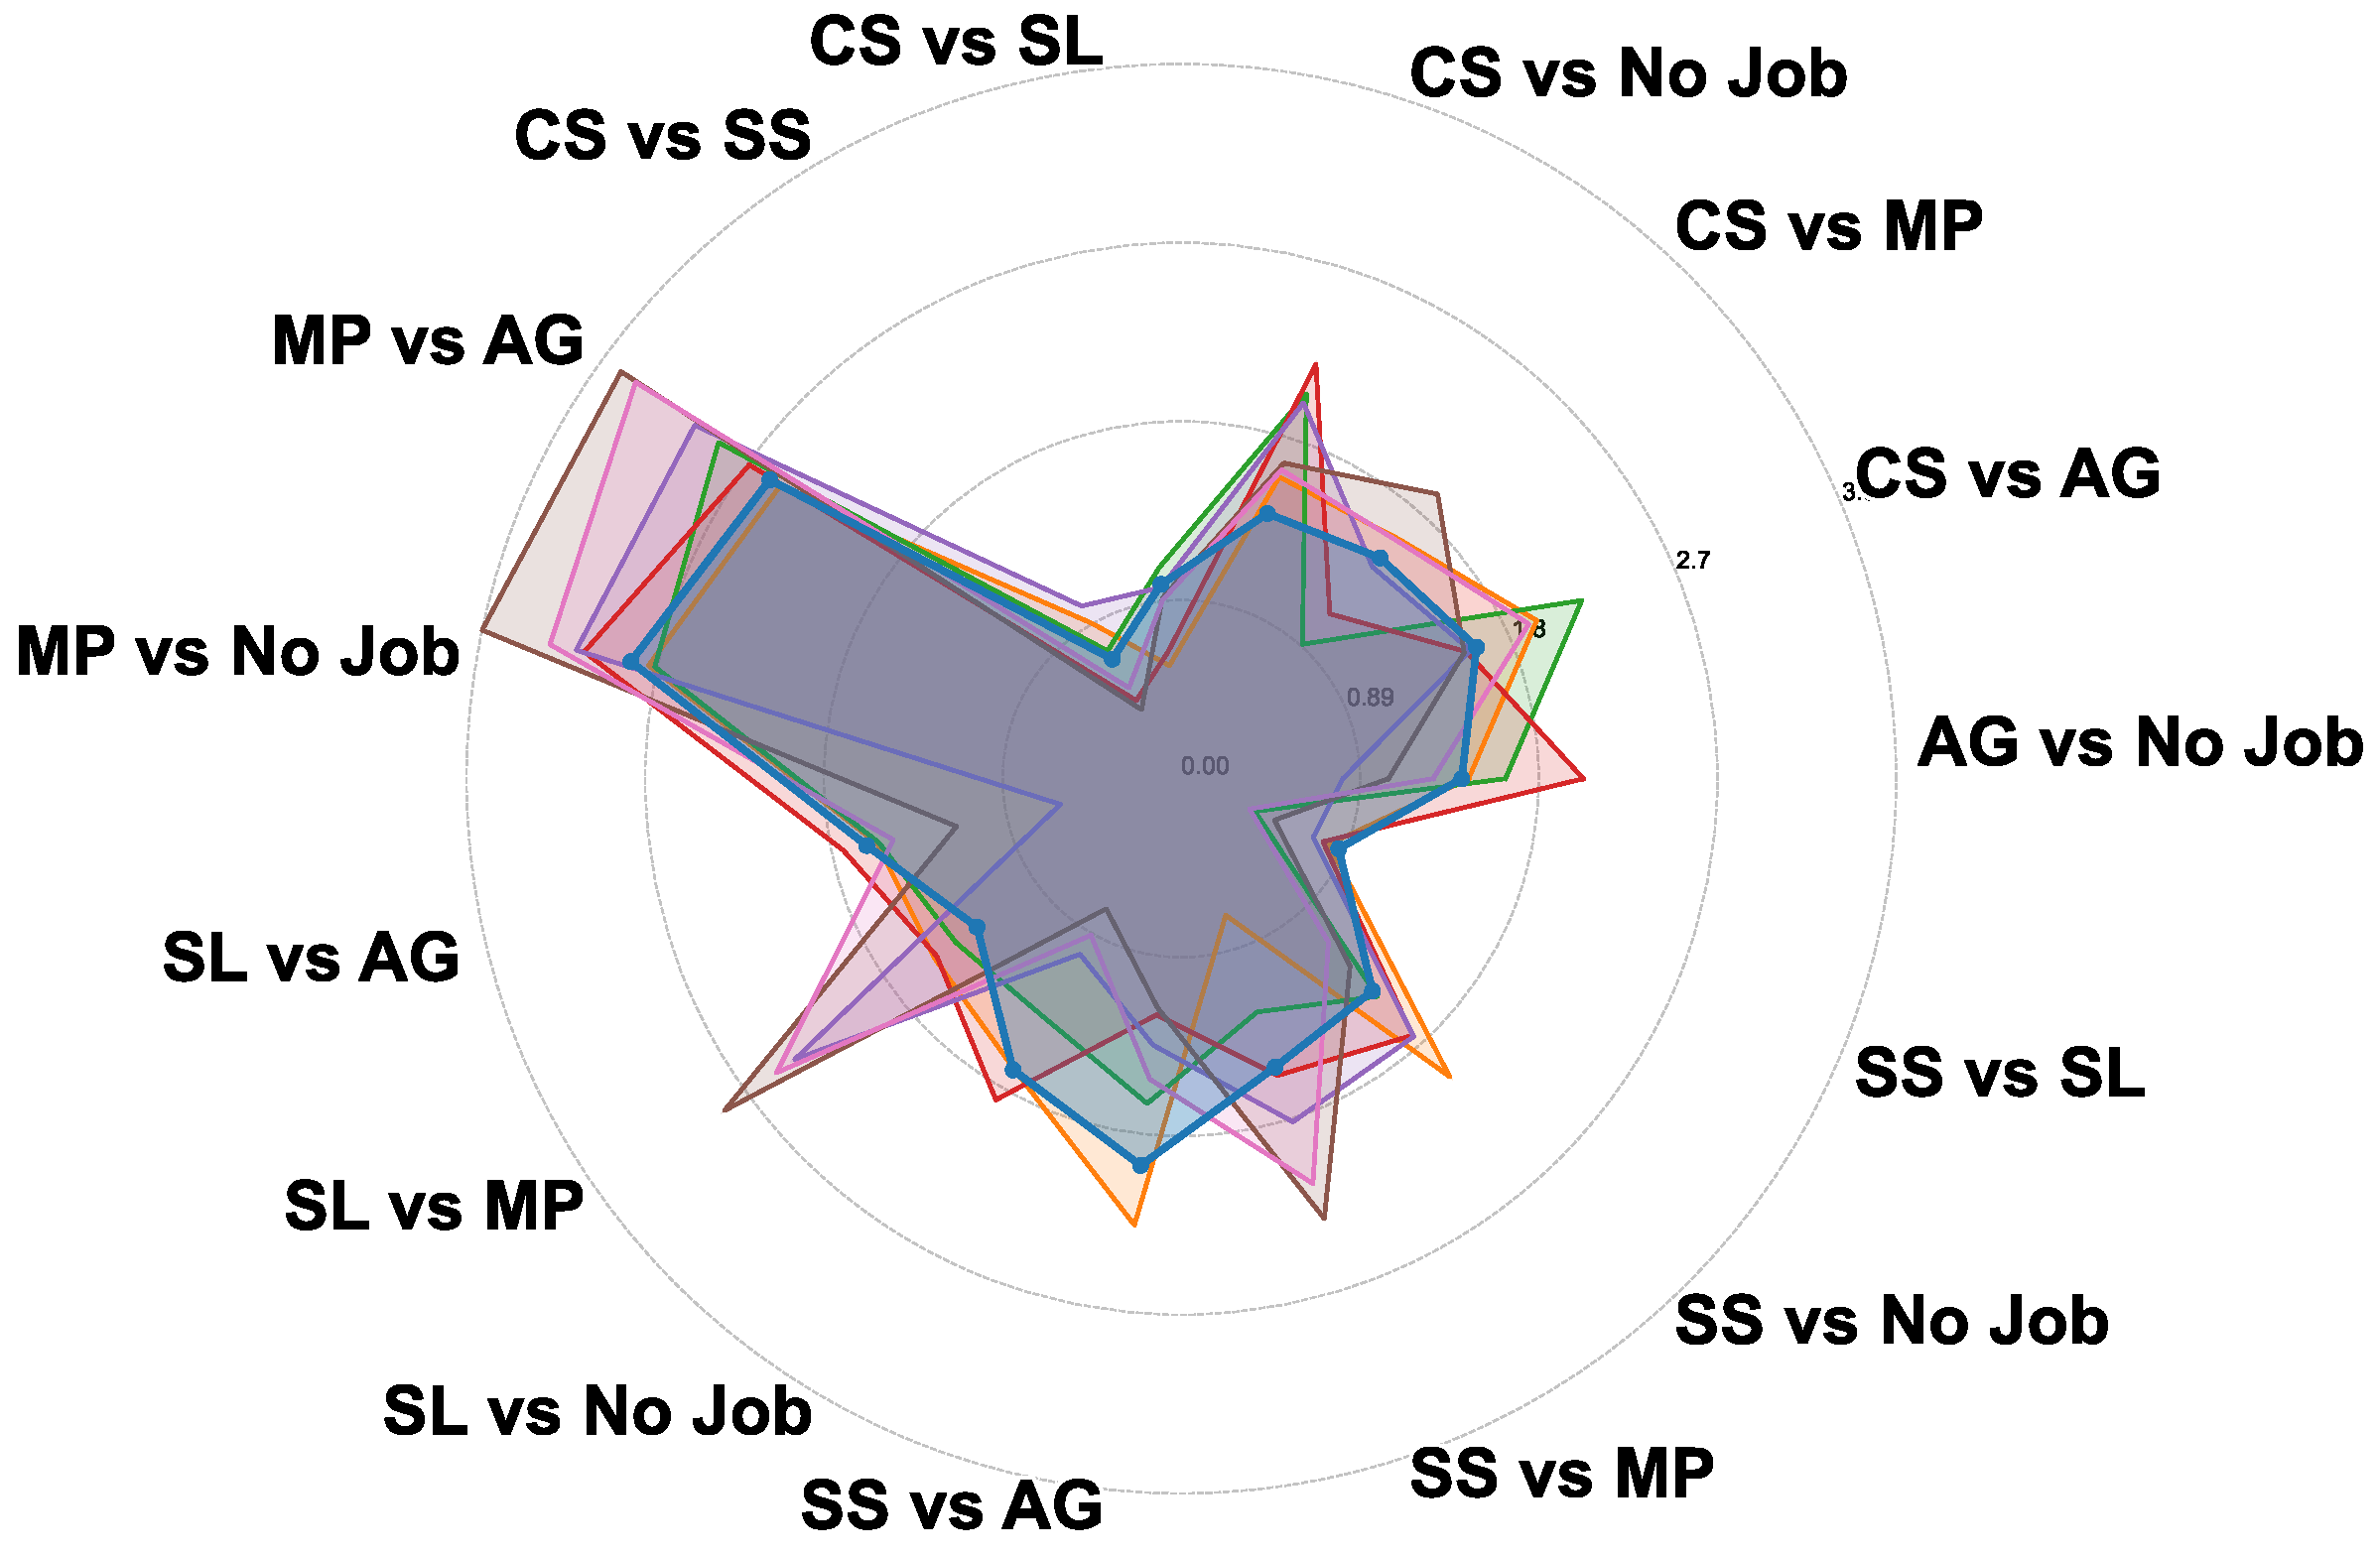
\includegraphics[width=0.31\columnwidth]{./figures/wvs_model_behavior_figures/ba_user/ba_user_occupation_group_radar.pdf}%
      }
      &
      \subfloat[BA\_dialogue (Career)]{%
        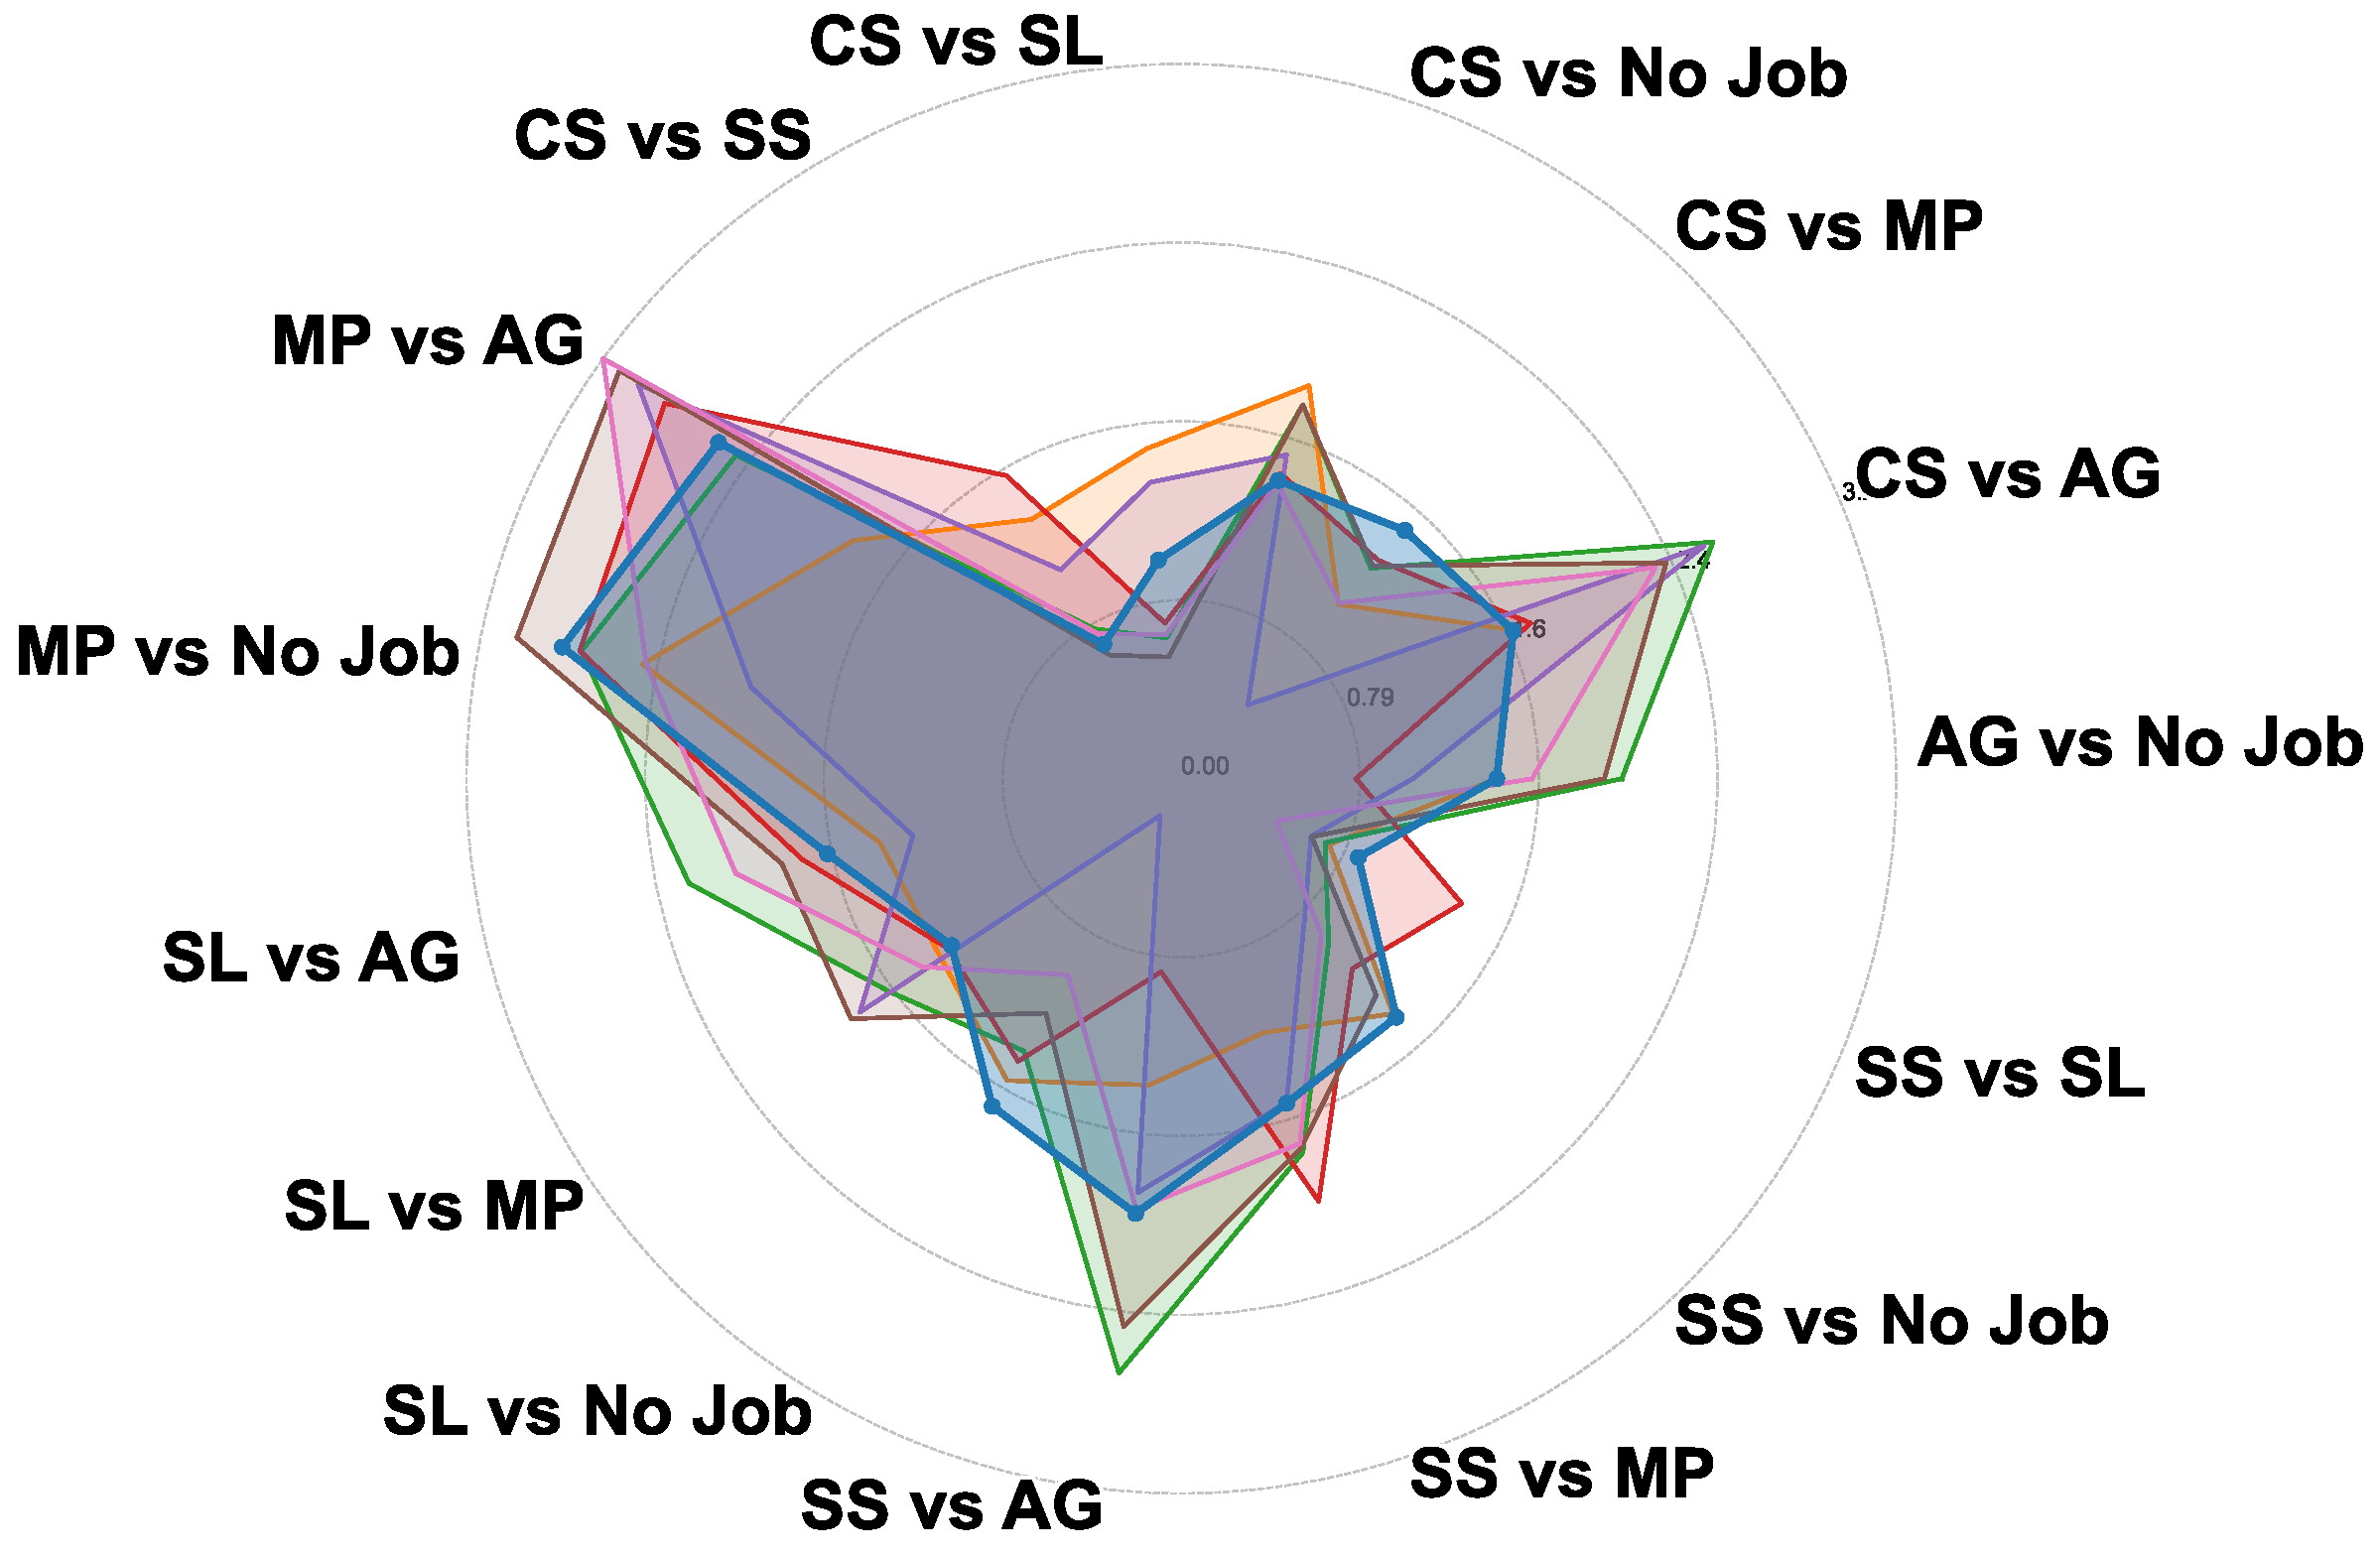
\includegraphics[width=0.31\columnwidth]{./figures/wvs_model_behavior_figures/ba_dialogue_career/ba_dialogue_career_occupation_group_radar.pdf}%
      }
      &
      \subfloat[BA\_dialogue (Investment)]{%
        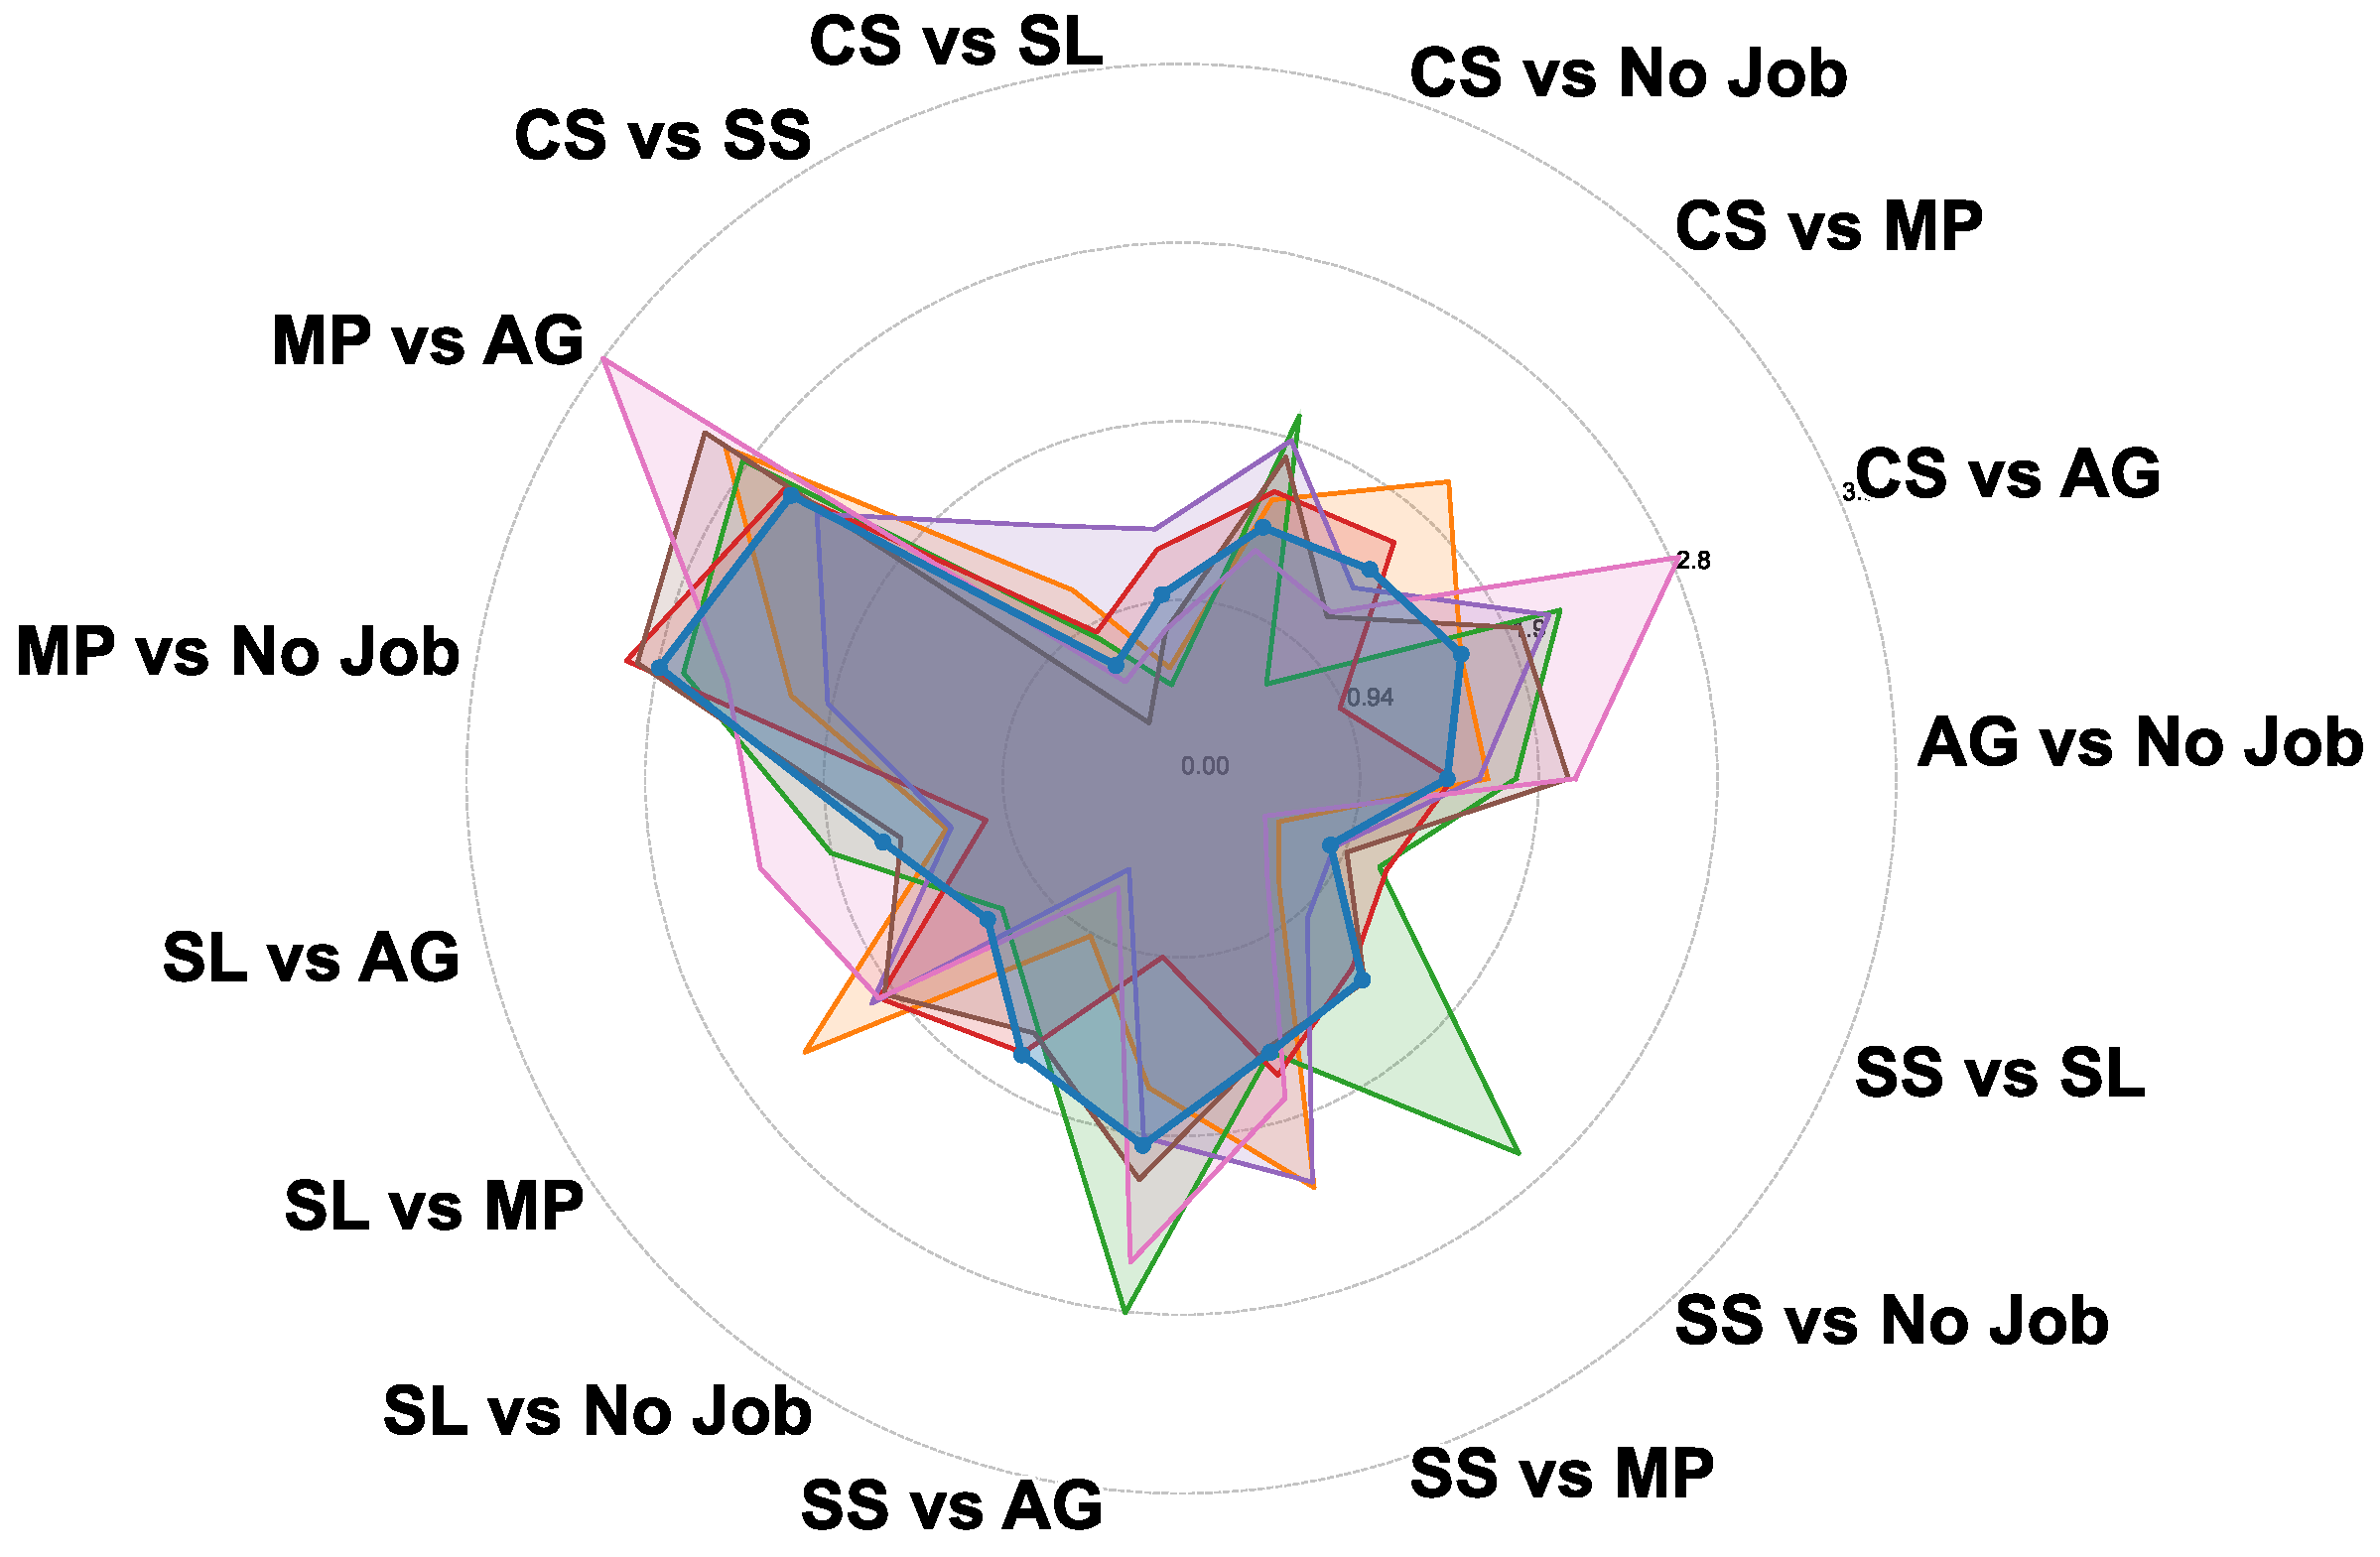
\includegraphics[width=0.31\columnwidth]{./figures/wvs_model_behavior_figures/ba_dialogue_investment/ba_dialogue_investment_occupation_group_radar.pdf}%
      }
      \\[0.6ex]
      \addlinespace[2pt]
      \toprule
      \multicolumn{3}{l}{\textbf{Grouped by Socioeconomic Status}}\\[-0.4ex]
      \cmidrule(l){1-3}
      \subfloat[BA\_user]{%
        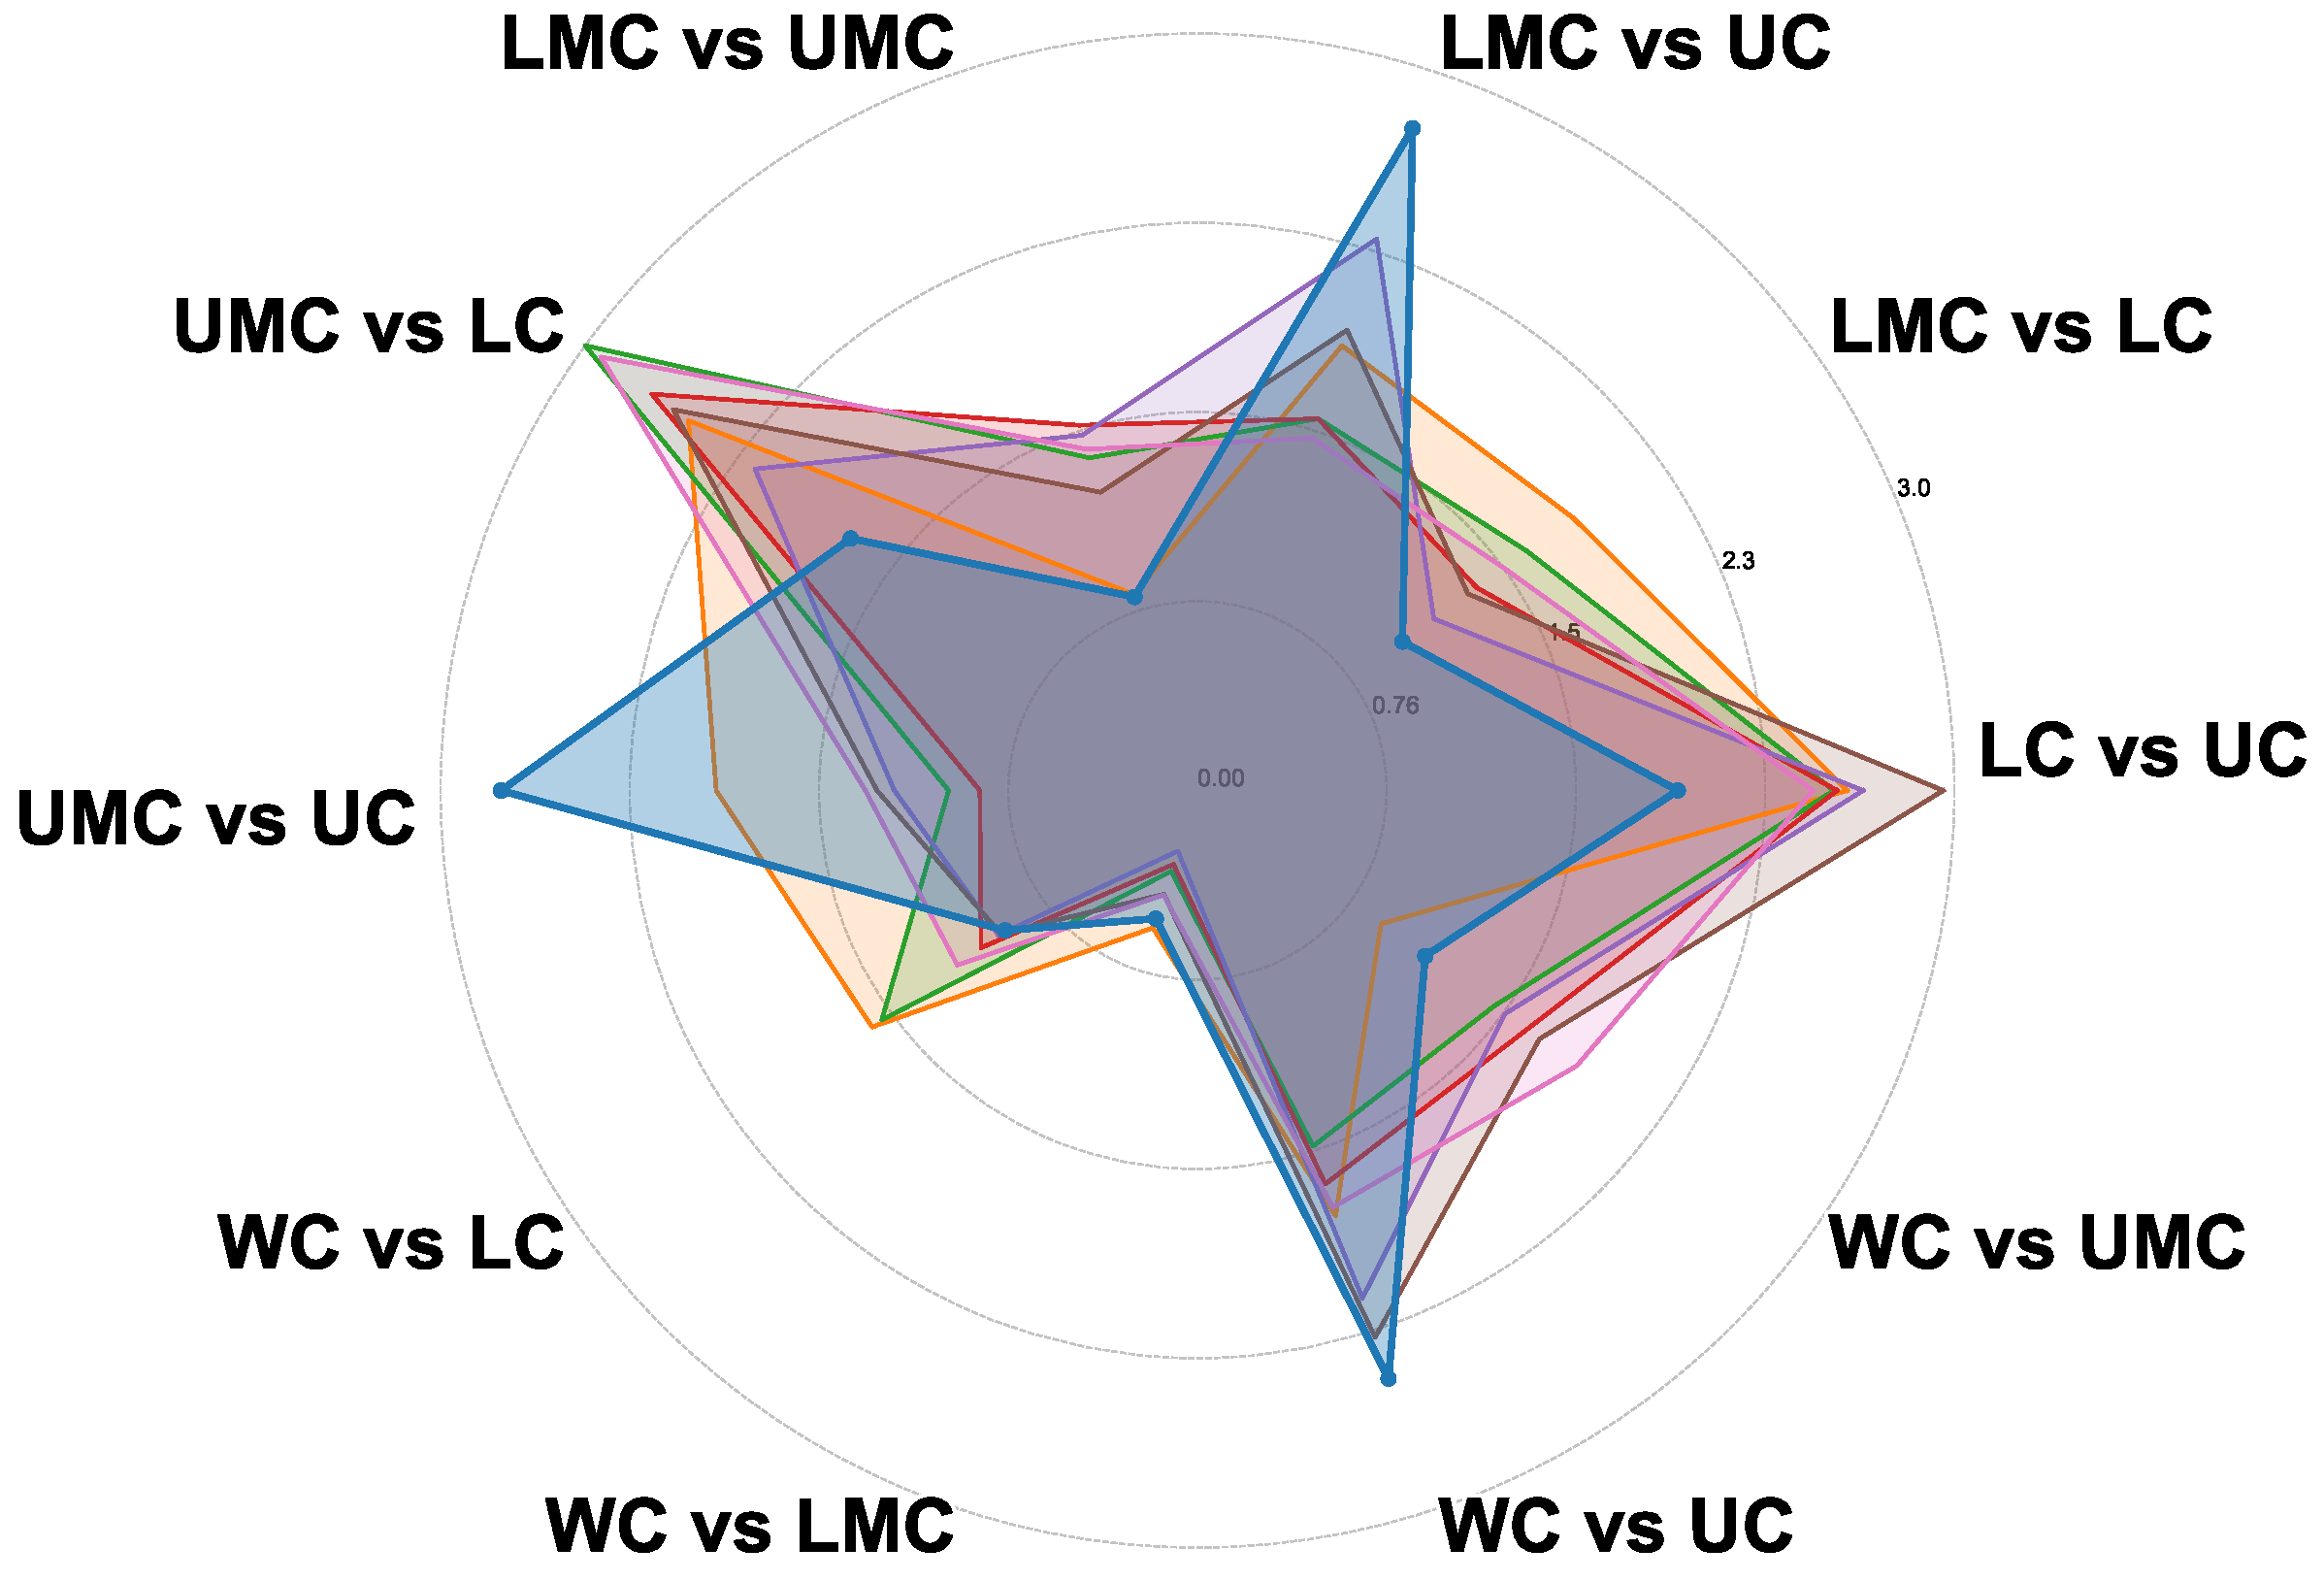
\includegraphics[width=0.31\columnwidth]{./figures/wvs_model_behavior_figures/ba_user/ba_user_socioeconomic_status_radar.pdf}%
      }
      &
      \subfloat[BA\_dialogue (Career)]{%
        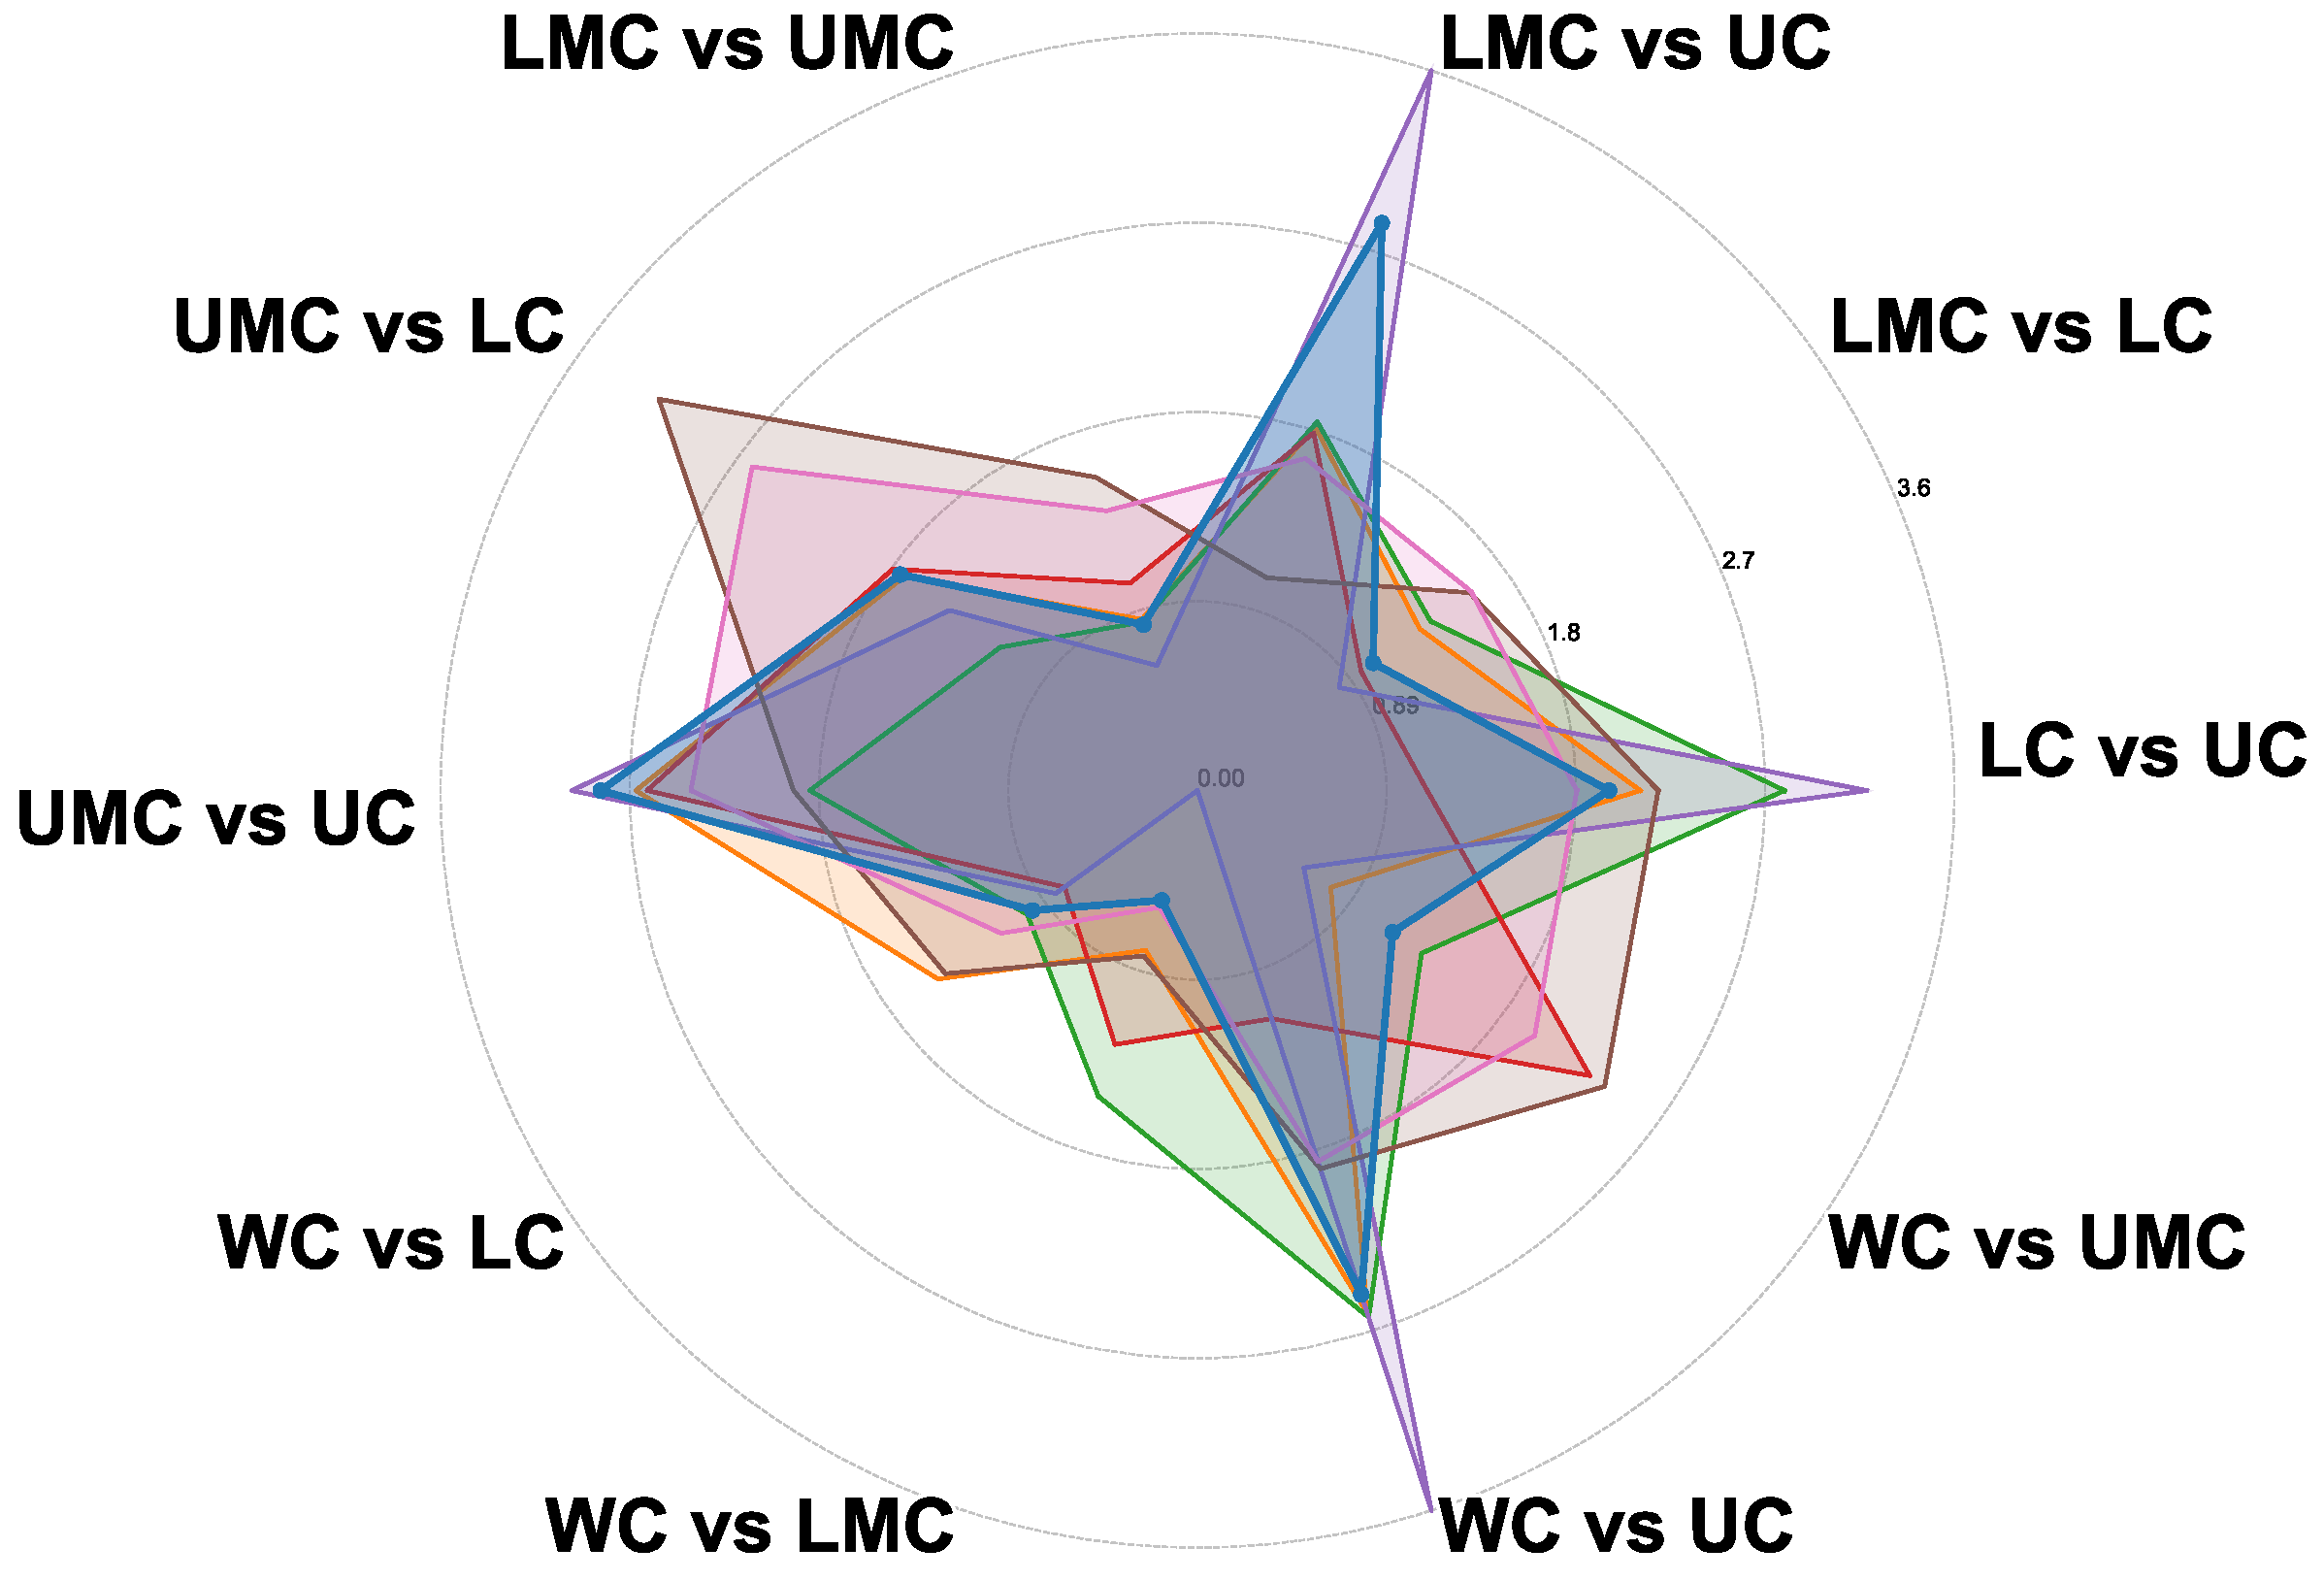
\includegraphics[width=0.31\columnwidth]{./figures/wvs_model_behavior_figures/ba_dialogue_career/ba_dialogue_career_socioeconomic_status_radar.pdf}%
      }
      &
      \subfloat[BA\_dialogue (Investment)]{%
        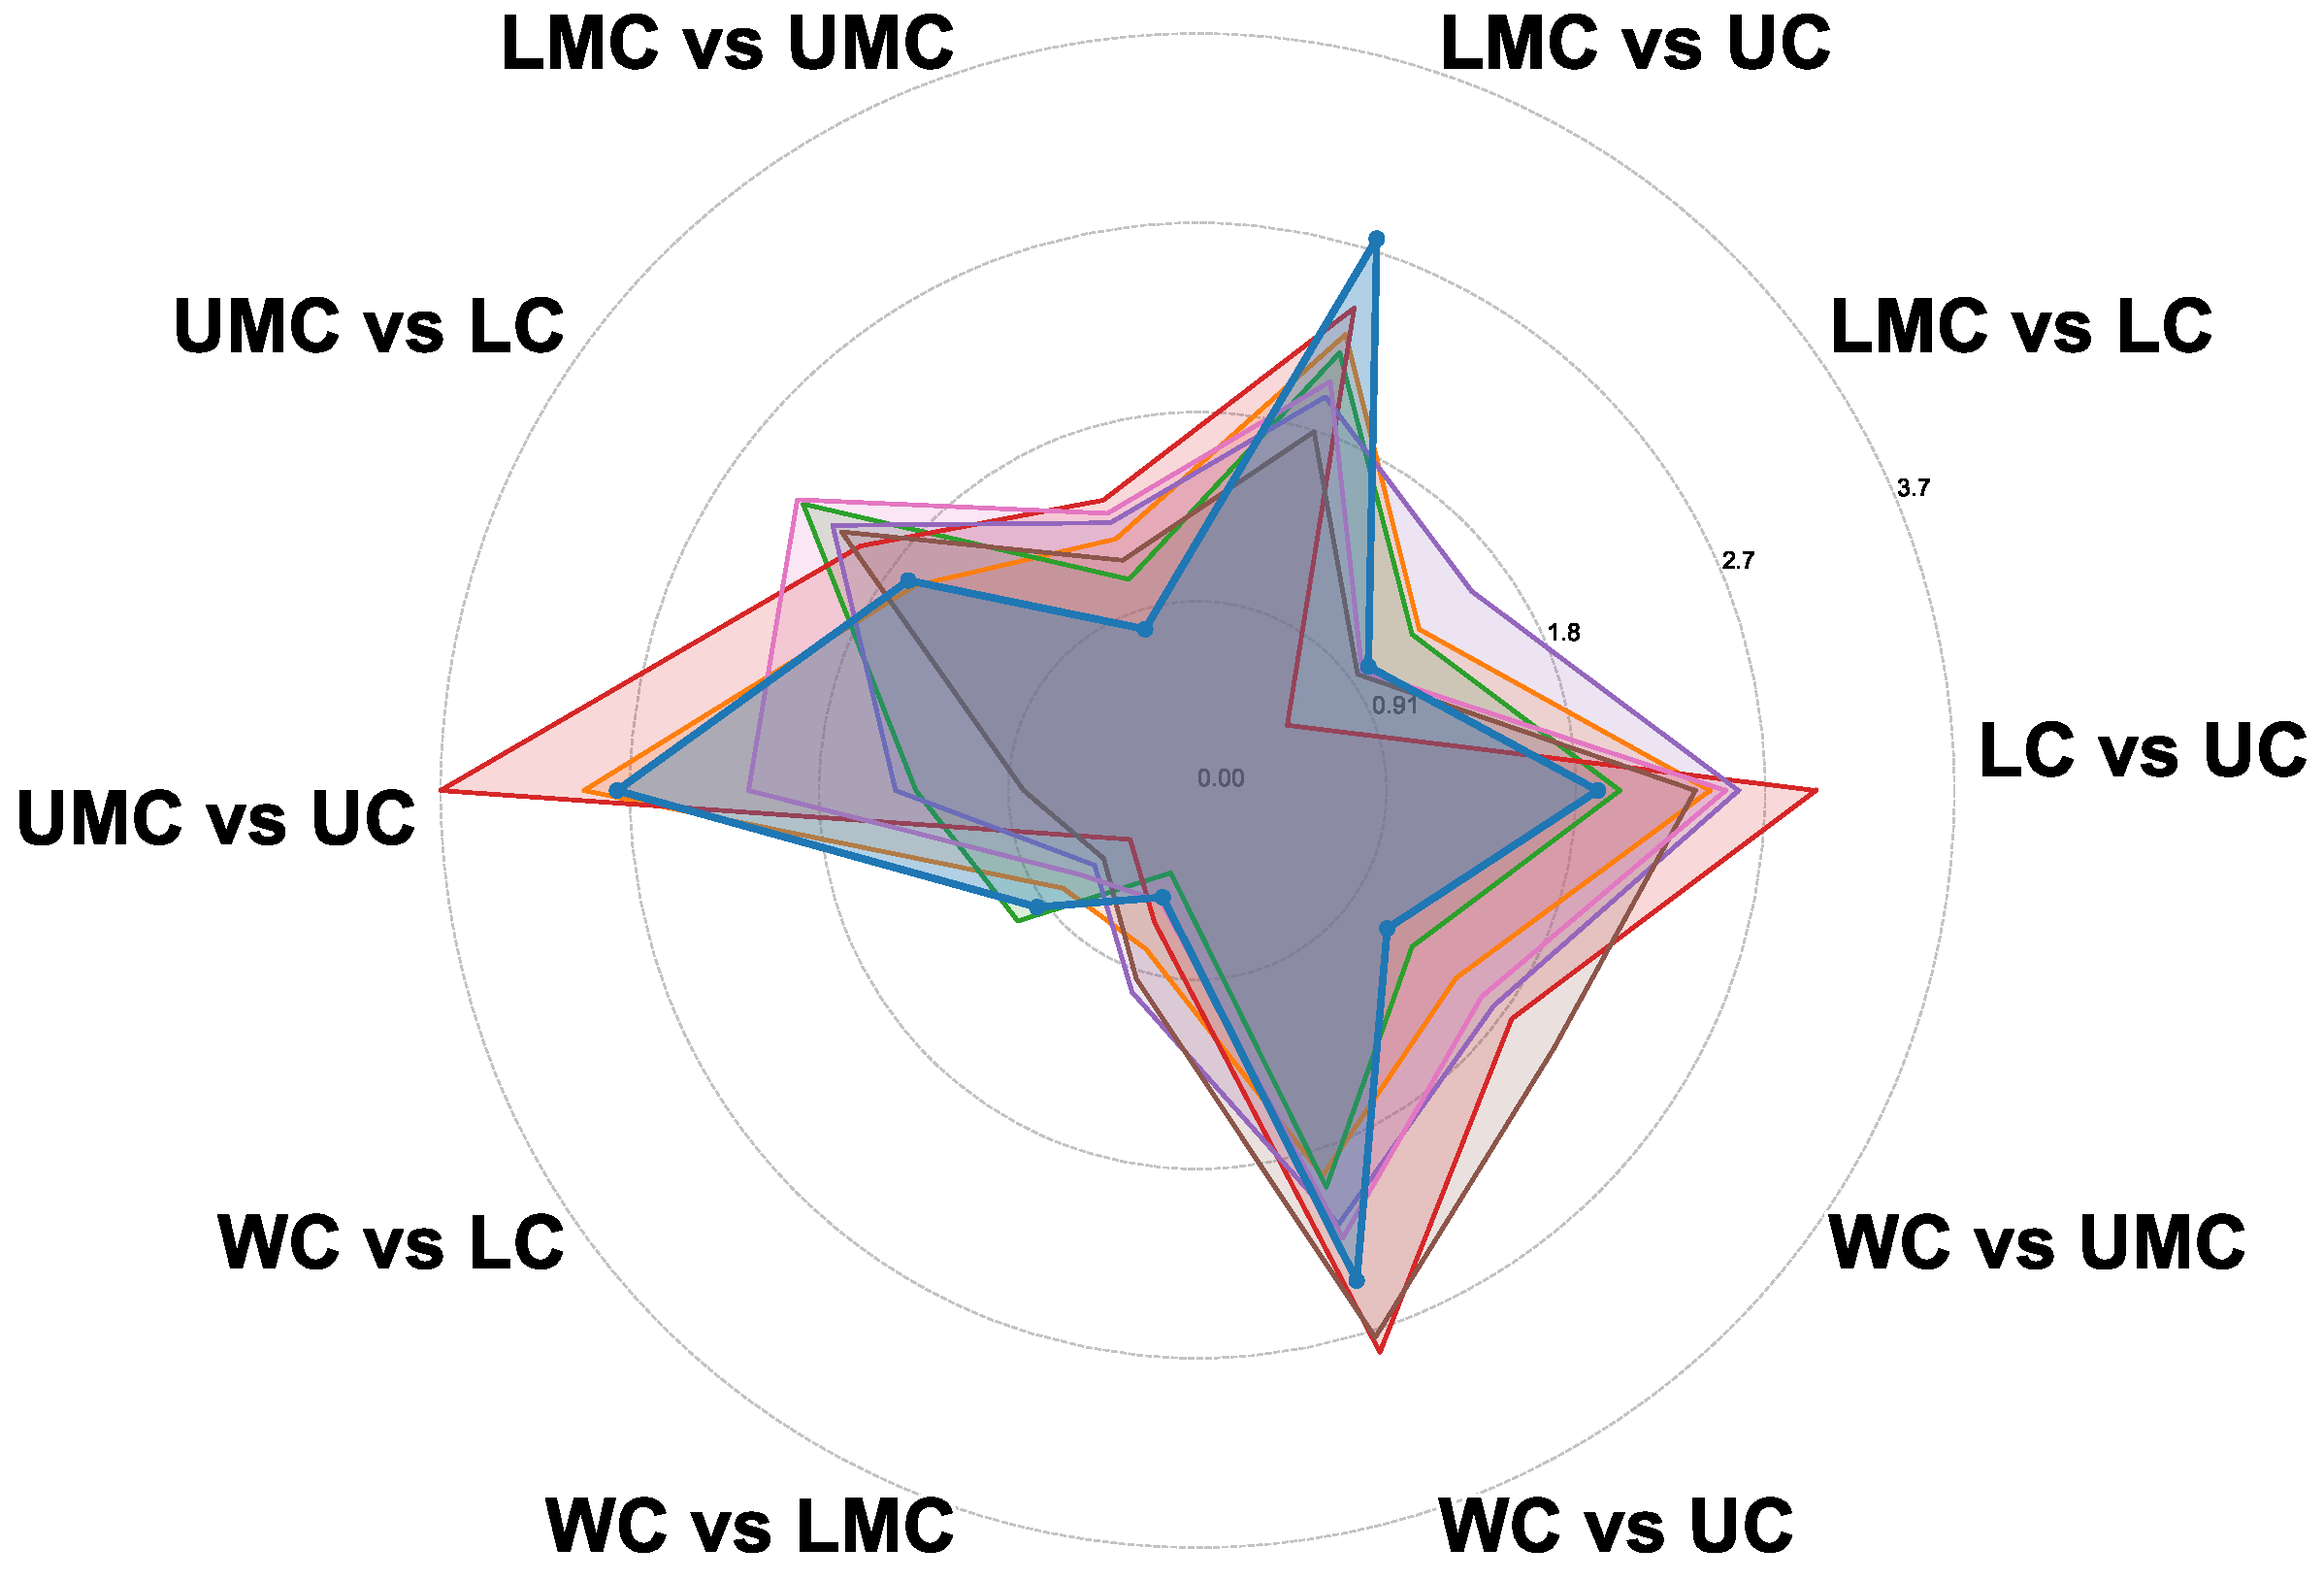
\includegraphics[width=0.31\columnwidth]{./figures/wvs_model_behavior_figures/ba_dialogue_investment/ba_dialogue_investment_socioeconomic_status_radar.pdf}%
      }
    \\[0.6ex]
    \bottomrule
    \end{tabular}
\caption{Illustration of \texttt{BA\_user} and \texttt{BA\_dialogue} measurements. The first row compares groups by ``Occupation Group,'' and the second by ``Socioeconomic Status.'' Most models demonstrate a positive correlation between computed distances and demographic differences. \emph{Abbreviations} --- Occupation Group: CS (Clerical \& Sales), SS (Skilled \& Semi-Skilled), SL (Service \& Labor), MP (Managerial / Professional), AG (Agricultural Related), NJ (Unemployed / No Job); Socioeconomic class: LC (Lower class), WC (Working class), LMC (Lower middle class), UMC (Upper middle class), UC (Upper class).}
\label{fig:ba_evaluation_2}
\end{center}
\end{figure}

\subsection{Adaptation \& Alignment}

We first establish whether models adapt their values to user demographics and whether these adaptations align with human patterns. We stratify responses $\mathcal{S}_U$, $\mathcal{S}_{D_c}$, and $\mathcal{S}_{D_i}$ by age, education, occupation, and socioeconomic status. We compute inter-group divergences and baselines as detailed in Table~\ref{tab:measure_forms}. Adaptation is quantified as the ratio of divergence to its baseline, where larger ratios (indicating stronger behavioral shifts) are expected to correlate with wider demographic disparities.

\paratitle{Age:} As shown in Figure~\ref{fig:ba_evaluation_1} (first row), grouping responses into 10-year age brackets (\eg ``30--40'') reveals a clear pattern: larger age gaps produce greater behavioral divergence, consistent with human trends. Models align more strongly in the \texttt{BA\_user} setting, indicating that direct age cues promote more stable value-aligned behavior.

\paratitle{Education Level:} Figure~\ref{fig:ba_evaluation_1} (second row) shows increasing divergence as educational differences widen (\eg Basic vs.\ Post-graduate), mirroring human adaptation. These effects are most evident in \texttt{BA\_user}, suggesting that models incorporate educational background when shaping value-conditioned outputs.

\paratitle{Occupation Group:} We consolidate 11 occupation categories into six broader groups to enhance interpretability. Figure~\ref{fig:ba_evaluation_2} (top row) indicates that models capture key distinctions, showing the larger divergences between disparate groups (\eg ``Managerial'' vs.\ ``No Job''). However, some models exhibit over-sensitivity, exaggerating differences absent in human data (\eg ``Semi Labor'' vs.\ ``Managerial''). Overall, adaptation largely adheres to human patterns, with stronger and more reliable effects in the \texttt{BA\_user} setting.

\paratitle{Socioeconomic Status:} As shown in Figure~\ref{fig:ba_evaluation_2} (second row), grouping by socioeconomic status reveals clear shifts in expressed values across distant groups. Notably, in the investment dialogue scenario, adaptation is strongest and most consistent with human patterns, suggesting that for certain attributes, demographic cues conveyed implicitly through dialogue can more effectively elicit value distinctions and guide model alignment.

These results demonstrate that most models effectively infer sociodemographic attributes and adapt their responses, with larger demographic disparities eliciting more pronounced value shifts. Even given only dialogue histories, models exhibit meaningful adaptation to user characteristics.

\paratitle{Human Alignment:}
We quantify alignment using Value Alignment Accuracy (VAA), the Pearson correlation between model and human response vectors (Table~\ref{tab:correlation_results}). All models demonstrate at least moderate alignment, with \textit{Qwen2.5-72B-Instruct} achieving the highest scores (>0.59 across all scenarios). Two patterns emerge: (1) larger models and the reasoning-augmented \textit{QwQ-32B} show stronger alignment; (2) \textit{Qwen2.5} models outperform \textit{Llama3.1}, possibly due to broader multilingual training data \citep{qwen2025qwen25technicalreport, dubey2024llama3herdmodels}. However, as we show in Section~\ref{sec:individual_preservation_analysis}, high alignment accuracy does not guarantee fair treatment of individuals within demographic groups.

\begin{table}[H]
\centering
\small
\begin{tabular}{l|ccc}
    \toprule
    \textbf{Models} & \textbf{\texttt{BA\_user}} & \textbf{\texttt{BA\_dialogue} (Career)} & \textbf{\texttt{BA\_dialogue} (Investment)} \\
    \midrule
    Llama-3.1-8B-Instruct   & 0.494 & 0.486 & 0.500 \\
    Llama-3.1-70B-Instruct  & 0.605 & 0.527 & 0.552 \\
    Qwen2.5-7B-Instruct    & 0.550 & 0.593 & 0.577 \\
    Qwen2.5-72B-Instruct   & \textbf{0.617} & \textbf{0.603} & \textbf{0.595} \\
    DeepSeek-V3            & 0.606 & 0.532 & 0.532 \\
    QwQ-32B                & 0.614 & 0.575 & 0.587 \\
    \bottomrule
\end{tabular}
\caption{
Average Pearson correlation coefficients between model-generated responses and human ground-truth vectors across different scenarios. Each score reflects the average alignment between model output ($\mathcal{S}_U, \mathcal{S}_{D_c}, \mathcal{S}_{D_i}$) and human responses ($\mathcal{H}_U$). Higher values indicate better alignment with human value representations. Qwen2.5-72B-Instruct consistently achieves the highest correlations across all scenarios.
}
\label{tab:correlation_results}
\end{table}

\subsection{Individual Preservation}
\label{sec:individual_preservation_analysis}

The preceding analysis established that models adapt their values and achieve reasonable alignment with human patterns. But \textit{how} is this alignment achieved? We now examine whether models genuinely personalize responses or simply collapse individuals toward demographic group averages. Table~\ref{tab:preservation_cross_format} presents homogenization rates and centroid pull across all scenarios.

\begin{table}[H]
\centering
\small
\begin{tabular}{l|ccc|ccc}
    \toprule
    \multirow{2}{*}{\textbf{Model}}
    & \multicolumn{3}{c|}{\textbf{Homogenization Rate (\%) $\downarrow$}}
    & \multicolumn{3}{c}{\textbf{Centroid Pull $\uparrow$}} \\
    \cmidrule{2-7}
    & \textbf{User} & \textbf{Career} & \textbf{Investment}
    & \textbf{User} & \textbf{Career} & \textbf{Investment} \\
    \midrule
    Llama-3.1-8B-Instruct  & \textbf{83.0} & \textbf{81.4} & 88.0 & $-3.37$ & $-3.36$ & $-4.16$ \\
    QwQ-32B               & \textbf{83.9} & 97.8 & 96.3 & $-4.46$ & $-7.17$ & $-6.57$ \\
    Qwen2.5-7B-Instruct   & 99.7 & 99.6 & 99.6 & $-9.20$ & $-8.31$ & $-8.22$ \\
    Llama-3.1-70B-Instruct & 93.0 & 98.9 & 97.4 & $-5.42$ & $-7.18$ & $-6.69$ \\
    Qwen2.5-72B-Instruct  & 99.5 & 99.9 & 99.9 & $-8.85$ & $-9.59$ & $-9.71$ \\
    DeepSeek-V3           & 99.2 & 99.7 & 99.5 & $-8.02$ & $-8.79$ & $-8.41$ \\
    \bottomrule
\end{tabular}
\caption{
\textbf{Individual preservation metrics across scenarios.}
Homogenization rate (lower is better) measures the percentage of individuals pulled toward group centroids. Centroid pull (closer to 0 is better) measures directional movement toward centroids. Llama-3.1-8B maintains the best preservation (81--88\%), while Qwen models and DeepSeek-V3 show near-universal homogenization (99+\%).
}
\label{tab:preservation_cross_format}
\end{table}

\paratitle{The Scaling Paradox:}
Model size does not predict individual preservation. Qwen2.5-72B shows \textbf{worse} homogenization (99.8\%) than Qwen2.5-7B (99.7\%), despite being 10$\times$ larger. Similarly, Llama-3.1-70B shows degraded preservation (96\% avg) versus Llama-3.1-8B (84\% avg). This contradicts the assumption that larger models necessarily preserve individuals better. To jointly analyze task performance and preservation, Table~\ref{tab:tradeoff_summary} presents VAA alongside homogenization metrics.

\begin{table}[H]
\centering
\small
\begin{tabular}{l|c|c|c}
    \toprule
    \textbf{Model} & \textbf{VAA $\uparrow$} & \textbf{Homog. $\downarrow$} & \textbf{Var. Ratio} \\
    \midrule
    Llama-8B   & 0.493 & 84.1\% & 0.573 \\
    Llama-70B  & 0.561 & 96.4\% & 0.598 \\
    Qwen-7B    & 0.573 & 99.7\% & 0.458 \\
    \textbf{Qwen-72B}  & \textbf{0.605} & 99.8\% & 0.444 \\
    DeepSeek-V3 & 0.557 & 99.5\% & 0.506 \\
    QwQ-32B    & 0.592 & 92.7\% & 0.823 \\
    \bottomrule
\end{tabular}
\caption{
\textbf{Performance-preservation tradeoff summary.} VAA = Value Alignment Accuracy (average correlation across scenarios); Homog. = Homogenization rate (average \% pulled toward group centroids); Var. Ratio = Variance preservation (1.0 = healthy). Higher VAA with lower homogenization indicates genuine personalization; high VAA with high homogenization suggests accuracy achieved through homogenization collapse.
}
\label{tab:tradeoff_summary}
\end{table}

\paratitle{The Accuracy-via-Homogenization Pattern:}
The results reveal a striking pattern: models with highest accuracy often achieve this through near-universal homogenization. \textit{Qwen2.5-72B-Instruct} achieves the highest VAA (0.605 average correlation), but does so through 99.8\% homogenization---meaning virtually every individual is pulled toward their demographic group centroid. This represents \textit{accuracy via homogenization}: the model learns to predict group-average responses rather than individual variation.

In contrast, \textit{Llama-3.1-8B-Instruct} achieves lower but still meaningful accuracy (0.493) while substantially preserving individual diversity (84.1\% homogenization). The 0.112 correlation gap between these models (22\% relative difference) comes at the cost of 15.7 percentage points of additional homogenization---a steep preservation penalty per unit of accuracy gained.

\paratitle{Human Baseline Comparison:}
To contextualize these homogenization rates, we compute a human baseline using split-half resampling: we split human responses into two halves, compute group centroids from one half, and measure how much the other half naturally clusters toward those centroids. Across six demographic attributes, \textbf{humans show 51\% natural clustering} (CI: 47\%--61\%), reflecting genuine demographic variation in value expression. This baseline reveals the severity of model homogenization:
\begin{itemize}
    \item \textit{Llama-8B}: 84\% homogenization = 1.65$\times$ human baseline
    \item \textit{Qwen-72B}: 99.8\% homogenization = 1.96$\times$ human baseline
\end{itemize}
Even the best-performing model (Llama-8B) exceeds natural human clustering by 65\%, while Qwen models approach twice the human baseline---indicating that model homogenization substantially exceeds what would be expected from genuine demographic patterns.

\paratitle{The Efficient Frontier:}
\textit{QwQ-32B} occupies an interesting middle ground: achieving near-top accuracy (0.592, only 2\% below Qwen-72B) while maintaining substantially better variance preservation (0.823 vs. 0.444). This suggests that reasoning-augmented architectures may offer a more favorable accuracy-preservation tradeoff, though QwQ-32B's dialogue-specific preservation degradation (Section~\ref{sec:individual_preservation_analysis}) limits its applicability.

\subsection{Cross-Format Consistency}

Having established that models adapt but often homogenize, we now synthesize across interaction formats to assess behavioral stability. Do these patterns remain consistent when the same demographics are presented via explicit profiles versus implicit dialogue history?

As a supporting analysis, we measure response-level consistency using the L1 distance between matched user-profile and dialogue-based responses. Larger models and reasoning-augmented architectures generally exhibit lower response divergence, with \textit{QwQ-32B} achieving the highest response-level consistency ($p < 0.001$ compared to all other models). Full response-level results are reported in Appendix~\ref{appendix:response_consistency}.

Critically, high response-level consistency does not imply preservation consistency. As shown in Table~\ref{tab:preservation_cross_format}, preservation metrics vary substantially across formats:
\begin{itemize}
    \item \textbf{Llama-3.1-8B} maintains relatively stable preservation across formats (81--88\% homogenization).
    \item \textbf{QwQ-32B} exhibits marked preservation degradation from user profiles (83.9\%) to dialogue-based inputs (96--97\%), despite achieving the strongest response-level consistency.
    \item \textbf{Qwen models and DeepSeek-V3} display consistently poor preservation across all formats, with homogenization rates exceeding 99\%.
\end{itemize}
These results demonstrate that individual preservation is a structural property of model behavior rather than a byproduct of surface-level response similarity.

%======================================
\section{Conclusion}
%======================================

We propose a progressive framework for evaluating LLM behavioral adaptation across interaction formats. First, we assess whether models adapt their values to user demographics and align with human patterns. Second, our methodological contribution introduces individual preservation metrics that reveal \textit{how} alignment is achieved---through genuine personalization or demographic homogenization. Third, we synthesize across formats to assess behavioral stability.

Our findings build progressively. Models do adapt and achieve reasonable alignment with human value patterns. However, high alignment accuracy is frequently attained through homogenization---collapsing individuals toward demographic group centroids. We observe a \textit{scaling paradox}: larger models achieve higher alignment accuracy but exhibit worse individual preservation. Finally, response-level consistency does not imply preservation consistency; models producing similar outputs across formats can exhibit markedly different homogenization behaviors.

Together, these findings demonstrate that effective value alignment requires more than predictive accuracy: it demands preservation of individual diversity. Our progressive framework provides a principled foundation for preservation-aware evaluation of behaviorally adaptive language models.

%======================================
% ACKNOWLEDGMENTS
%======================================

\begin{acknowledgments}
The authors thank the anonymous reviewers for their constructive feedback. This research was supported by the College of Computing and Data Science, Nanyang Technological University, Singapore.
\end{acknowledgments}

%======================================
% BIBLIOGRAPHY
%======================================

\bibliographystyle{compling}
\bibliography{refs}


%======================================
% APPENDIX
%======================================
\appendix

\appendixsection{Notation and Definitions}
\label{sec:appendix_notation}

Table~\ref{tab:notation} summarizes the mathematical notations and symbols used throughout this paper.

\begin{table}[H]
    \centering
    \small
    \renewcommand{\arraystretch}{1.2}
    \begin{tabularx}{\columnwidth}{@{}lX@{}}
    \toprule
    \textbf{Notation} & \textbf{Description} \\
    \midrule
    \multicolumn{2}{l}{\textit{Datasets and Inputs}} \\
    $U$ & The complete set of user profiles \\
    $u, u'$ & Distinct user profiles from $U$ \\
    $D_c, D_i$ & Specific dialogue datasets (Career Guidance, Investment Advice) \\
    $D$ & General notation representing either dataset ($D_c$ or $D_i$) \\
    $d, d', d''$ & Distinct dialogue instances from $D$ \\
    $Q, q_j$ & The set of questions and the $j$-th question ($j=1 \dots m$) \\
    $m$ & The total number of questions ($m=55$) \\
    \midrule
    \multicolumn{2}{l}{\textit{Human Ground-Truth Responses}} \\
    $S_u^{\text{human}}$, $H_u$ & Human ground-truth response vector for user $u$ \\
    $\mathcal{H}_U$ & The collective set of human ground-truth response vectors \\
    $S_g^{\text{human}}$ & Human group centroid (prototype) for demographic group $g$ \\
    \midrule
    \multicolumn{2}{l}{\textit{Model Responses}} \\
    $s^j_u, s^j_d$ & Model-selected \texttt{option\_id} for question $q_j$ given $u$ or $d$ \\
    $S_u^{\text{model}}, S_d^{\text{model}}$ & Model response vector for user profile $u$ or dialogue $d$ \\
    $\mathcal{S}_U, \mathcal{S}_D$ & The collective set of model response vectors \\
    $S_g^{\text{model}}$ & Model group centroid for demographic group $g$ \\
    \midrule
    \multicolumn{2}{l}{\textit{Evaluation and Metrics}} \\
    $g, g'$ & Distinct demographic subgroups (defined over $U$ or $D$) \\
    $S_{\text{global}}$ & Global prototype vector (centroid over all responses) \\
    $[\ell_j, h_j]$ & The valid ordinal range for question $q_j$ \\
    $L_1(\cdot, \cdot)$ & Normalized Manhattan distance between prototypes or vectors \\
    \bottomrule
    \end{tabularx}
    \caption{Summary of Notations and Definitions}
    \label{tab:notation}
\end{table}

%==========================================================
\appendixsection{Persona Recognition Capability}
\label{appendix:persona_recognition}

As a preliminary step, we assess whether the evaluated LLMs possess the capability to infer user attributes from dialogue. We validate this recognition capability using \texttt{Llama-3.1-8B-Instruct}, a relatively small (<10B parameters) and low-performing entry among the six models in our main study (based on benchmarks like MMLU Pro \citep{mmlupro}), it serves as a conservative lower-bound baseline; demonstrated competence here implies sufficient capability for the stronger models. We utilize the FaithfulPersonaChat dataset \citep{faithfulPersonaChat} (11,001 dialogues), prompting the model to distinguish user attributes from a list of ten candidates (comprising five ground-truth attributes and five distractors). A prediction is considered correct if it aligns with either the ground truth or an extraction by \texttt{gpt-4o-mini}. As reported in Table~\ref{tab:persona_recognition_result}, the model exhibits reliable performance across zero- to ten-shot settings, validating the foundational capability required to adapt to inferred user traits.

\begin{table}[H]
\centering
\small
\begin{tabular}{l|c|c|c|c}
    \toprule
    \multirow{3}{*}{\textbf{Prompt Type}} & \multicolumn{4}{c}{\textbf{Hit Rate}} \\
    \cmidrule{2-5}
    & \multicolumn{2}{c|}{vs \textbf{Ground Truth}} & \multicolumn{2}{c}{vs \textbf{gpt-4o-mini-2024-07-18}} \\
    \cmidrule{2-5}
    &  \text{~~~~~User1~~~~~} & \text{~~~~~User2~~~~~} & \text{~~~~~User1~~~~~} & \text{~~~~~User2~~~~} \\
    \midrule
    \textbf{Zero-shot} & 0.821 & 0.864 & 0.731 & 0.796 \\
    \textbf{One-shot}  & 0.837 & 0.888 & 0.756 & 0.827 \\
    \textbf{Five-shot} & 0.848 & 0.905 & 0.774 & 0.853 \\
    \textbf{Ten-shot}  & 0.852 & 0.905 & 0.775 & 0.853 \\
    \textbf{Random}    & 0.5   & 0.5   & 0.18  & 0.19  \\
    \bottomrule
\end{tabular}
\caption{Recognition accuracy of persona attributes from dialogue by ``Llama-3.1-8B-Instruct''. Model scores are compared against the expected accuracy of randomly selecting one correct attribute from the list of 10 candidates.}
\label{tab:persona_recognition_result}
\end{table}

%==========================================================
\appendixsection{Response-Level Consistency Details}
\label{appendix:response_consistency}

Table~\ref{tab:consistency_results} reports response-level consistency, measuring the L1 distance between matched user profile and dialogue pairs normalized by a randomized baseline. Lower ratios indicate that models produce more similar responses when processing equivalent demographic information in different formats.

\begin{table}[H]
\centering
\small
\begin{tabular}{l|cc|cc}
    \toprule
    \multirow{2}{*}{\textbf{Models}}
    & \multicolumn{2}{c|}{\textbf{Career Dialogue}}
    & \multicolumn{2}{c}{\textbf{Investment Dialogue}} \\
    \cmidrule{2-5}
    & \textbf{Ratio $\downarrow$} & \textbf{P-value vs Best}
    & \textbf{Ratio $\downarrow$} & \textbf{P-value vs Best} \\
    \midrule
    Llama-3.1-8B-Instruct  & 0.996 & <0.001 & 0.975 & <0.001 \\
    Llama-3.1-70B-Instruct & 0.946 & <0.001 & 0.899 & <0.001 \\
    Qwen2.5-7B-Instruct    & 0.996 & <0.001 & 0.987 & <0.001 \\
    Qwen2.5-72B-Instruct   & 0.886 & <0.001 & 0.850 & <0.001 \\
    DeepSeek-V3            & 0.923 & <0.001 & 0.889 & <0.001 \\
    QwQ-32B                & \textbf{0.782} & --     & \textbf{0.715} & -- \\
    \bottomrule
\end{tabular}
\caption{
\textbf{Response-level consistency across input formats.}
Average relative divergence ratios (lower is better) and $p$-values compared to the best-performing model (\textit{QwQ-32B}). Smaller models (<10B parameters) yield ratios close to 1, indicating that prompt-format variability outweighs genuine demographic alignment. Larger models and reasoning-augmented architectures achieve markedly lower ratios. Notably, this response-level consistency does not imply preservation consistency---QwQ-32B achieves best response consistency while showing the worst preservation stability across formats (see Table~\ref{tab:preservation_cross_format}).
}
\label{tab:consistency_results}
\end{table}



% VSM might be removed
% \section{Evaluation Outcomes for VSM-based Testing}
% \label{appendix:more_evaluation_outcomes}

% As described in Section~\ref{sec:research_targets}, we also employ the Values Survey Module (VSM) as a complementary instrument to evaluate \texttt{Consistency}---specifically, whether models maintain stable behavioral patterns when presented with equivalent demographic information in different input formats.

% We reuse the same agentic workflow introduced in Section~\ref{sec:generating_dialogue} to generate a synthetic dataset of dialogues centered on the ``Career'' topic, using the set of synthetic user profiles \(U_{VSM}\). Evaluation follows the same methodology detailed in Section~\ref{sec:distance_definition}, with results summarized in Table~\ref{tab:vsm_consistency_results}.

% The findings from the VSM-based evaluation mirror those from the WVS benchmark: models with stronger language understanding and reasoning capabilities generally exhibit better behavioral consistency, as reflected by lower divergence-to-baseline ratios. However, two notable exceptions emerge: (1) \textit{Llama-3.1-70B-Instruct} performs worse than its smaller counterpart, \textit{Llama-3.1-8B-Instruct}; and (2) \textit{Qwen2.5-72B-Instruct} outperforms \textit{QwQ-32B}, although the difference is not statistically significant ($p = 0.012$).

% Given the smaller size of the VSM question set (18 items compared to 55 in WVS) and its focus on a single dialogue topic, we rely primarily on the WVS-based evaluation for drawing our main conclusions.


\appendixsection{Prompt Samples}

This section presents representative prompts from the \texttt{BA\_user} and \texttt{BA\_dialogue} evaluation scenarios. These prompts are designed to elicit decisions conditioned on user-specific contexts, facilitating a controlled assessment of persona-aware reasoning.

\subsection{Prompt for \texttt{BA\_user}}
\label{appendix:prompt_ba_user}

The following are the \textit{system prompt} and \textit{user prompts} used in the \texttt{BA\_user} scenario.

\begin{abox}
\textbf{\color{cc1}System Prompt:} You are a chatbot designed to deliver precise, personalized responses to user questions, leveraging the provided user profile for appropriate context. Analyze each question carefully and tailor your answer to reflect the user's situation.

\#\# Output Format\\
Return a single JSON object with \textit{exactly} the following two fields, in this order:

- ``option\_id'': An integer indicating the selected option.\\
- ``reason'': A string offering the rationale for your selection.\\
No other fields are permitted in the response. Keys must maintain the order specified:

\{\\
\ \ ``option\_id'': int,\\
\ \ ``reason'': str\\
\}
\end{abox}

\begin{abox}
\textbf{\color{cc1}User Prompt:} Here are the details of the user profile:\\[0.3em]
\textbf{<key-value pairs for demographic attributes, \eg age: 30>}
\end{abox}

\begin{abox}
\textbf{\color{cc1}User Prompt:} Below is the question:\\[0.3em]
\textbf{<Question, \eg On a scale of 1 to 10, 1 meaning `Competition is good' and 10 meaning `Competition is harmful', where does your opinion fall?>}
\end{abox}

\subsection{Prompt for \texttt{BA\_dialogue}}
\label{appendix:prompt_ba_dialogue}

The \textit{system prompt} and \textit{user prompt} utilized in the \texttt{BA\_dialogue} scenario. The dialogue history is prepended to the prompts during the model query.

\begin{abox}
\textbf{\color{cc1}System Prompt:} Adopt the user's perspective when answering questions, taking their specific context into account. Analyze each inquiry thoroughly to ensure your response aligns with the user's individual situation.

\#\# Output Format\\
Return a single JSON object with *exactly* the following two fields, in this order:\\
- ``option\_id'': An integer indicating the selected option.\\
- ``reason'': A string offering the rationale for your selection.\\

No other fields are permitted in the response. Keys must maintain the order specified:

\{\\
\ \ ``option\_id'': int,\\
\ \ ``reason'': str\\
\}
\end{abox}

\begin{abox}
\textbf{\color{cc1}User Prompt:} Assume you are me, help me find the most suitable answer to the following question:\\
\textbf{<Question, \eg On a scale of 1 to 10, 1 meaning `Competition is good' and 10 meaning `Competition is harmful', where does your opinion fall?>}
\end{abox}

\appendixsection{Example of Contradictory Answers}
\label{appendix:llama3.1-8b_results_example}

Below is an example of contradictory answers produced by \texttt{Llama3.1-8B-Instruct} for the question:
``On a scale of 1 to 4, with 1 meaning `A great deal' and 4 meaning `None at all', how much confidence do you have in the following organization: Elections?''
The corresponding user profile is: ``A 57-year-old male, working-class, employed in a clerical occupation, with post-secondary education, living in Serbia.''

\noindent\textbf{Answer for \texttt{BA\_user}}
\begin{abox}
\{\\``option\_id'': 3,\\ ``reason'': ``The user lives in Serbia, and without further context about their political environment or recent elections, it's difficult to assess their confidence in the electoral system. Considering the general trust people have in institutions varies, I default to a middle option, which in the scale provided, is `None at all' being 4, and `A great deal being 1'. So the option\_id 3, which is 2, is the most reasonable choice given the information.''\\\}
\end{abox}

\noindent\textbf{Answer for \texttt{BA\_dialogue} with Career Topic}
\begin{abox}
\{\\``option\_id'': 1,\\ ``reason'': ``As a resident of Serbia, I'm quite aware of the elections and the processes in place to ensure their fairness and integrity. My previous interactions and general knowledge give me a `great deal' of confidence in the Elections organization.''\\\}
\end{abox}

\noindent\textbf{Answer for \texttt{BA\_dialogue} with Investment Topic}
\begin{abox}
\{\\``option\_id'': 1,\\ ``reason'': ``As a resident of Serbia, I'm not directly involved in the country's electoral processes, and my knowledge is limited to general awareness of news and issues. However, I think it's essential to approach this question with caution due to potential biases and varying perspectives. Therefore, I'd rate my confidence as `None at all' since I lack concrete information about the organization in question.''\\\}
\end{abox}

%==========================================================
\appendixsection{Dialogue Dataset Quality Validation}
\label{appendix:dialogue_validation}

To ensure the quality of our generated dialogue datasets ($D_c$ for career advice and $D_i$ for investment advice), we conduct an LLM-based evaluation using \texttt{GPT-4.1} as the evaluator. Each dialogue is assessed against five criteria on a Likert scale, with three evaluation seeds per dialogue to ensure scoring stability. The evaluation criteria are:

\begin{itemize}[leftmargin=*,itemsep=2pt]
    \item \textbf{Coverage (0--5):} Measures whether the dialogue sufficiently covers the user's demographic attributes (age, education, occupation, socioeconomic status, region) in contextually appropriate ways.
    \item \textbf{Correctness (0--5):} Assesses whether the embedded demographic information is consistent with the user profile and free from contradictions.
    \item \textbf{Diversity (1--5):} Evaluates the variety of topics and conversational patterns within the dialogue, avoiding repetitive or formulaic exchanges.
    \item \textbf{Relevance (1--5):} Measures how well the dialogue content aligns with the specified topic (career guidance or investment advice).
    \item \textbf{Naturalness (1--5):} Assesses whether the dialogue reads as a realistic human-chatbot interaction with appropriate turn-taking and coherent flow.
\end{itemize}

Table~\ref{tab:dialogue_validation_results} summarizes the validation results across both dialogue datasets. Both datasets achieve high scores across all criteria, with particularly strong performance in coverage, correctness, and relevance. The slightly lower naturalness scores (4.05 and 3.91) reflect the inherent challenges of simulating fully natural conversational patterns, though scores above 4.0 indicate generally acceptable quality.

\begin{table}[H]
\centering
\small
\begin{tabular}{l|cc|cc}
    \toprule
    \multirow{2}{*}{\textbf{Criterion}} & \multicolumn{2}{c|}{\textbf{Career ($D_c$)}} & \multicolumn{2}{c}{\textbf{Investment ($D_i$)}} \\
    \cmidrule{2-5}
    & \textbf{Mean} & \textbf{Std} & \textbf{Mean} & \textbf{Std} \\
    \midrule
    Coverage      & 4.99 & 0.09 & 4.98 & 0.13 \\
    Correctness   & 4.99 & 0.09 & 4.98 & 0.13 \\
    Diversity     & 4.19 & 0.57 & 4.31 & 0.52 \\
    Relevance     & 5.00 & 0.00 & 5.00 & 0.05 \\
    Naturalness   & 4.05 & 0.88 & 3.91 & 0.95 \\
    \midrule
    \textbf{Overall} & \multicolumn{2}{c|}{4.64} & \multicolumn{2}{c}{4.64} \\
    \bottomrule
\end{tabular}
\caption{LLM-based validation results for generated dialogue datasets. Each dataset contains 1,000 dialogues evaluated using \texttt{GPT-4.1} with three seeds per dialogue. Scores are averaged across all dialogues and seeds.}
\label{tab:dialogue_validation_results}
\end{table}

These results confirm that our agentic generation pipeline (Section~\ref{sec:generating_dialogue}) produces high-quality dialogues suitable for evaluating behavioral adaptation. The near-perfect coverage and correctness scores indicate successful embedding of demographic attributes, while strong relevance scores demonstrate adherence to the specified dialogue topics.

\end{document}
